%%%% kr-instructions.tex -- version 1.2 (27-Feb-2020)

\typeout{Forgetting in CTL to Compute Necessary and Sufficient Conditions}

% These are the instructions for authors for KR-20.

\documentclass{article}
\pdfpagewidth=8.5in
\pdfpageheight=11in

\usepackage{kr}

% Use the postscript times font!
\usepackage{times}
\usepackage{soul}
\usepackage{url}
\usepackage[hidelinks]{hyperref}
\usepackage[utf8]{inputenc}
\usepackage[small]{caption}
\usepackage{graphicx}
\usepackage{amsmath}
\usepackage{amsthm}
\usepackage{booktabs}
%\usepackage{algorithm}
%\usepackage{algorithmic}

\usepackage{enumerate}
\usepackage[linesnumbered,boxed]{algorithm2e}
\usepackage{amstext}
\usepackage{amssymb}
\usepackage{color}

\urlstyle{same}


\usepackage{tikz}
\usetikzlibrary{automata}

% the following package is optional:
%\usepackage{latexsym}

% See https://www.overleaf.com/learn/latex/theorems_and_proofs
% for a nice explanation of how to define new theorems, but keep
% in mind that the amsthm package is already included in this
% template and that you must *not* alter the styling.
\newtheorem{example}{Example}
\newtheorem{theorem}{Theorem}

% Following comment is from ijcai97-submit.tex:
% The preparation of these files was supported by Schlumberger Palo Alto
% Research, AT\&T Bell Laboratories, and Morgan Kaufmann Publishers.
% Shirley Jowell, of Morgan Kaufmann Publishers, and Peter F.
% Patel-Schneider, of AT\&T Bell Laboratories collaborated on their
% preparation.

% These instructions can be modified and used in other conferences as long
% as credit to the authors and supporting agencies is retained, this notice
% is not changed, and further modification or reuse is not restricted.
% Neither Shirley Jowell nor Peter F. Patel-Schneider can be listed as
% contacts for providing assistance without their prior permission.

% To use for other conferences, change references to files and the
% conference appropriate and use other authors, contacts, publishers, and
% organizations.
% Also change the deadline and address for returning papers and the length and
% page charge instructions.
% Put where the files are available in the appropriate places.

\title{On Sufficient and Necessary Conditions in Bounded \CTL: A Forgetting Approach}
	%Forgetting in CTL to Compute Necessary and Sufficient Conditions}

% Single author syntax
\iffalse % (remove the multiple-author syntax below and \iffalse ... \fi here)
\author{%
    Author name
    \affiliations
    Affiliation
    \emails
    email@example.com    % email
}
\fi
% Multiple author syntax
\author{%
Renyan Feng$^{1,2}$\and
Erman Acar$^{2,*}$\and
Stefan Schlobach$^{2}$\and
Yisong Wang$^{1,}$\footnote{Corresponding author(s).} \and
Wanwei Liu $^3$\\
\affiliations
$^{1}$Guizhou University, P. R. China\\
$^{2}$Vrije Universiteit Amsterdam, Netherlands\\
$^{3}$National University of Defense Technology, P. R. China\\
%$^3$Third Affiliation\\
%$^4$Fourth Affiliation \\
\emails
fengrenyan@gmail.com,
\{Erman.Acar, k.s.schlobach\}@vu.nl,
yswang@gzu.edu.cn,
wwliu@nudt.edu.cn
}

\begin{document}

\newcommand{\tuple}[1]{{\langle{#1}\rangle}}
\newcommand{\Mod}{\textit{Mod}}
\newcommand\ie{{\it i.e. }}
\newcommand\eg{{\it e.g.}}
%\newcommand\st{{\it s.t. }}
\renewcommand{\st}{s.t.}
\newtheorem{definition}{Definition}
%\newtheorem{examp}{Example}
%\newenvironment{example}{\begin{examp}\rm}{\end{examp}}
\newtheorem{lemma}{Lemma}
\newtheorem{proposition}{Proposition}
%\newtheorem{theorem}{Theorem}
\newtheorem{corollary}[theorem]{Corollary}
%\newenvironment{proof}{{\bf Proof:}}{\hfill\rule{2mm}{2mm}\\ }
\newcommand{\rto}{\rightarrow}
\newcommand{\lto}{\leftarrow}
\newcommand{\lrto}{\leftrightarrow}
\newcommand{\Rto}{\Rightarrow}
\newcommand{\Lto}{\Leftarrow}
\newcommand{\LRto}{\Leftrightarrow}
\newcommand{\Var}{\textit{Var}}
\newcommand{\Forget}{\textit{Forget}}
\newcommand{\KForget}{\textit{KForget}}
\newcommand{\TForget}{\textit{TForget}}
%\newcommand{\forget}{\textit{forget}}
\newcommand{\Fst}{\textit{Fst}}
\newcommand{\dep}{\textit{dep}}
\newcommand{\term}{\textit{term}}
\newcommand{\literal}{\textit{literal}}

\newcommand{\Atom}{\mathcal{A}}
\newcommand{\SFive}{\textbf{S5}}
\newcommand{\MPK}{\textsc{k}}
\newcommand{\MPB}{\textsc{b}}
\newcommand{\MPT}{\textsc{t}}
\newcommand{\MPA}{\forall}
\newcommand{\MPE}{\exists}

\newcommand{\DNF}{\textit{DNF}}
\newcommand{\CNF}{\textit{CNF}}

\newcommand{\degree}{\textit{degree}}
\newcommand{\sunfold}{\textit{sunfold}}

\newcommand{\Pos}{\textit{Pos}}
\newcommand{\Neg}{\textit{Neg}}
\newcommand\wrt{{\it w.r.t.}}
\newcommand{\Hm} {{\cal M}}
\newcommand{\Hw} {{\cal W}}
\newcommand{\Hr} {{\cal R}}
\newcommand{\Hb} {{\cal B}}
\newcommand{\Ha} {{\cal A}}

\newcommand{\Dsj}{\triangledown}

\newcommand{\wnext}{\widetilde{\bigcirc}}
\newcommand{\nex}{\bigcirc}
\newcommand{\ness}{\square}
\newcommand{\qness}{\boxminus}
\newcommand{\wqnext}{\widetilde{\circleddash}}
\newcommand{\qnext}{\circleddash}
\newcommand{\may}{\lozenge}
\newcommand{\qmay}{\blacklozenge}
\newcommand{\unt} {{\cal U}}
\newcommand{\since} {{\cal S}}
\newcommand{\SNF} {\textit{SNF$_C$}}
\newcommand{\start}{\textbf{start}}
\newcommand{\Elm}{\textit{Elm}}
\newcommand{\simp}{\textbf{simp}}
\newcommand{\nnf}{\textbf{nnf}}

\newcommand{\CTL}{\textrm{CTL}}
\newcommand{\Ind}{\textrm{Ind}}
\newcommand{\Tran}{\textrm{Tran}}
\newcommand{\Sub}{\textrm{Sub}}
\newcommand{\NI}{\textrm{NI}}
\newcommand{\Inst}{\textrm{Inst}}
\newcommand{\Com}{\textrm{Com}}
\newcommand{\Rp}{\textrm{Rp}}
\newcommand{\forget}{{\textsc{f}_\CTL}}
\newcommand{\ALL}{\textsc{a}}
\newcommand{\EXIST}{\textsc{e}}
\newcommand{\NEXT}{\textsc{x}}
\newcommand{\FUTURE}{\textsc{f}}
\newcommand{\UNTIL}{\textsc{u}}
\newcommand{\GLOBAL}{\textsc{g}}
\newcommand{\UNLESS}{\textsc{w}}
\newcommand{\Def}{\textrm{def}}
\newcommand{\IR}{\textrm{IR}}
\newcommand{\Tr}{\textrm{Tr}}
\newcommand{\dis}{\textrm{dis}}
\def\PP{\ensuremath{\textbf{PP}}}
\def\NgP{\ensuremath{\textbf{NP}}}
\def\W{\ensuremath{\textbf{W}}}
\newcommand{\Pre}{\textrm{Pre}}
\newcommand{\Post}{\textrm{Post}}


\newcommand{\CTLsnf}{{\textsc{SNF}_{\textsc{ctl}}^g}}
\newcommand{\ResC}{{\textsc{R}_{\textsc{ctl}}^{\succ, S}}}
\newcommand{\CTLforget}{{\textsc{F}_{\textsc{ctl}}}}
\newcommand{\degex}{{\textsc{def}_{\textsc{ex}}}}
\newcommand{\Refine}{\textsc{Refine}}
\newcommand{\cf}{\textrm{cf.}}
\newcommand{\NEXP}{\textmd{\rm NEXP}}
\newcommand{\EXP}{\textmd{\rm EXP}}
\newcommand{\coNEXP}{\textmd{\rm co-NEXP}}
\newcommand{\NP}{\textmd{\rm NP}}
\newcommand{\coNP}{\textmd{\rm co-NP}}
\newcommand{\Pol}{\textmd{\rm P}}
\newcommand{\BH}[1]{\textmd{\rm BH}_{#1}}
\newcommand{\coBH}[1]{\textmd{\rm co-BH}_{#1}}
\newcommand{\Empty}{\emptyset}%\varnothing}
\newcommand{\NLOG}{\textmd{\rm NLOG}}
\newcommand{\DeltaP}[1]{\Delta_{#1}^{p}}
\newcommand{\PIP}[1]{\Pi_{#1}^{p}}
\newcommand{\SigmaP}[1]{\Sigma_{#1}^{p}}



\maketitle
%\textcolor{cyan}{NOTE: the \textcolor{red}{``red sentences"} in this paper is a new one added by myself; the \textcolor{blue}{``blue sentences"} is the one i want to replace by the \textcolor{red}{``red sentences"}; the \textcolor{green}{``green sentences"} is the one i want to delete. Besides, I have rewritten the Introduction.}

\begin{abstract}
Computation Tree Logic (\CTL) is one of the central formalisms in formal verification. As a specification language, it is used to express a property
that the system at hand is expected to satisfy. From
both the verification and the system design points
of view, some information content of such property might become irrelevant for the system due to
various reasons, e.g., it might become obsolete by
time, or perhaps infeasible due to practical difficulties. Then, the problem arises on how to subtract such piece of information without altering the
relevant system behaviour or violating the existing
specifications over a given signature. Moreover, in such a scenario, two
crucial notions are informative: the strongest necessary condition (SNC) and the weakest sufficient
condition (WSC) of a given property.


To address such a scenario in a principled way, we
introduce a forgetting-based approach in \CTL\ and
show that it can be used to compute SNC and WSC
of a property under a given model and over a given signature. We study its
theoretical properties and also show that our notion
of forgetting satisfies existing essential postulates of knowledge forgetting.
Furthermore, we analyse the computational complexity of some basic reasoning tasks for the fragment $\CTL_{\ALL\FUTURE}$ in particular.
%including various results for the relevant fragment $\CTL_{\ALL\FUTURE}$.
\end{abstract}

\section{Introduction}
\label{introduction}
%example

Computation Tree Logic (\CTL)~\cite{clarke1981design} is one of the central formalisms in formal verification. As a specification language, it is used to express a property
that the system at hand is expected to satisfy. From
both the verification and the system design points
of view,  there might be situations in which some information content of such property might become irrelevant for the system due to various reasons e.g., it might be discarded or become obsolete by time, or just  become infeasible due to practical difficulties. As keeping such information would be highly space-inefficient, the problem arises on how to remove it without altering the
relevant system behaviour or violating the existing system
specifications over a given signature. Consider the following example.

\begin{example}[Car-Manufacturing Company]\label{car_manufacturing}
Assume a car-manufacturing company which produces two types of cars: a (se)dan car and a (sp)orts car. In each manufacturing cycle, the company has to (s)elect one of the three options: (1) produce $se$  first, and then $sp$; (2) produce $sp$ first, and then $se$; (3) produce $se$ and $sp$ at the same time. At the end of each selection, a final (d)ecision is taken.

In Figure~\ref{BVM}, this scenario is  represented by the Kripke structure $\Hm=(S, R, L)$ with the initial state $s_0$ (called labelled state transition graph),  and the corresponding atomic variables $V=\{d,s,se,sp\}$.
\begin{figure}[ht]
  \centering
  % Requires \usepackage{graphicx}
  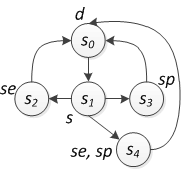
\includegraphics[width=3cm]{NnewCar.png}\\
  \caption{Car Engine Manufacturing Scenario }\label{BVM}
\end{figure}
Now assume a situation in which due to some problems (e.g., economic crises or new environmental regulations on the engine technology) company can no longer support the production of sports cars.
This means, all the manufacturing processes concerning $sp$ are no more necessary and should be dropped from both the specifications and the Kripke structure for simplification.
\end{example}
%State names are depicted inside the rounds and the label of each state is next to the round of corresponding state.
%Moreover, $s_0$ is the initial state where the leader decide to how many sedan cars and sports cars should be produced respectively.
%State $s_1$ selects producing \emph{sedan cars} which corresponds to the state $s_2$ or producing \emph{sports cars} which corresponds to the state $s_3$ or producing both sedan and sports cars which corresponds to the state $s_4$.


%Since every time the production is finished, the leaders needs to accept the cars, after each production state ($s_2$ or $s_3$ or $s_4$), we turn back to the initial state ($s_0$) to start over.
% In this case, we should have a specification, $\EXIST \NEXT(se \wedge lc \wedge sr)$, for the production sedan car and a specification, $\EXIST \NEXT(le \wedge sr)$, for the sports car.
%Let $\varphi=\ALL\GLOBAL \ALL \FUTURE(sr)$, which means $sr$ will be satisfied infinitely many times in the structure, be a \CTL\ formula.


% \begin{figure}[ht]
%   \centering
% \begin{tikzpicture}[shorten >= 1pt, node distance = 1.5cm, auto]
% \node[state] (s_0) [above of=s_1] [label=$d$]      {$s_0$};
% \node[state] (s_1)  [label=$s$]   {$s_1$};
% \node[state] (s_2) [left of=s_1] [label=$se$] {$s_2$};
% \node[state] (s_3) [right of=s_1] [label=$sp$]  {$s_3$};
% \node[state] (s_4) [below right of=s_1]  [label=${se,sp}$] {$s_4$};

% \path[->] (s_0) edge node {} (s_1)
%           (s_1) edge node {} (s_2)
%           (s_1) edge node {} (s_3)
%           (s_1) edge node {} (s_4)
%           (s_2) edge node {} (s_0)
%           (s_3) edge node {} (s_0)
%           (s_4) edge node {} (s_0);
% % rankdir=LR;
% % size="8,5"
% % node [shape = circle];
% % $s_0$ -> $s_1$;
% % $s_1$ -> $s_2$;
% % $s_1$ -> $s_3$;
% % $s_1$ -> $s_4$;
% % $s_2$ -> $s_0$;
% % $s_3$ -> $s_0$;
% \end{tikzpicture}
% \caption{Car Engine Manufacturing Scenario }\label{BVM}
% \end{figure}


Similar scenarios  like the one presented in Example~\ref{car_manufacturing} may arise in many different domains such as business-process modelling, software development, concurrent systems and more~\cite{Baier:PMC:2008}. Yet dropping some restrictions in a large and complex  system or specification, without affecting the working system components or violating dependent specifications over a given signature, is a non-trivial task.   Moreover, in such a scenario, two logical notions introduced by E. Dijkstra in~\cite{DBLP:journals/cacm/Dijkstra75} are highly informative: the \emph{strongest necessary condition} (SNC) and the \emph{weakest sufficient condition}  (WSC)  of a given specification. These correspond to the \emph{most general consequence} and the \emph{most specific abduction} of such specification, respectively.
%\textcolor{red}{This will be discussed in more depth later.}

%original example
% Consider a car-manufacturing company which produces two types of automobiles: a sedan car (basically a four-doored classical passenger car) and a sports car.  No matter a sedan or a sports car, both production lines are subject to a single standard criterion which is indispensable: safety restrictions.  This shared feature is also complemented several major differences aligned with these types in general. That is, a sedan car is produced with a small engine, while a sports car is produced with a large one. Moreover, due to its large amount of production, the sedan car is subject to some very restrictive low-carbon emission regulations, while a sports car is not.

% This scenario can be easily represented  as a small example by the following the Kripke structure $\Hm=(S, R, L)$ in Figure~\ref{BVM} on $V=\{ sl, sr, se, le, lc\}$ whose elements correspond to  \emph{select},  \emph{safety restrictions}, \emph{small engine},  \emph{large engine} and \emph{low-carbon emission requirements}, respectively.
% States are represented by  rounds and transitions by solid lines with arrow.
% State names are depicted inside the rounds and the label of each state is next to the round of corresponding state.
% Moreover, $s_0$ is the initial state where we select either choose producing an engine for \emph{sedan} which corresponds to the state $s_1$ or a \emph{sports car} which corresponds to the state $s_2$.
% Since only a single-type of production is possible at a time, after each production state ($s_1$ or $s_2$), we turn back to the initial state ($s_0$) to start over.
% In this case, we should have a specification, $\EXIST \NEXT(se \wedge lc \wedge sr)$, for the production sedan car and a specification, $\EXIST \NEXT(le \wedge sr)$, for the sports car.
% %Let $\varphi=\ALL\GLOBAL \ALL \FUTURE(sr)$, which means $sr$ will be satisfied infinitely many times in the structure, be a \CTL\ formula.
% \begin{figure}[ht]
%   \centering
%   % Requires \usepackage{graphicx}
%   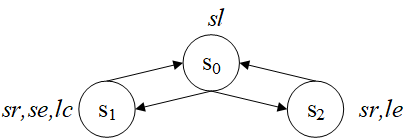
\includegraphics[width=5cm]{BVM.png}\\
%   \caption{Car Engine Manufacturing Scenario }\label{BVM}
% \end{figure}


% On the verge of shifting to an upcoming new engine technology, the company aims to adapt the sedan production to electrical engines.
% This means that electric sedans are not subject to low-carbon emission restrictions any more and hence such standardis obsolete, and can be dropped from both the specifications and the Kripke structure to simplify.
% Yet dropping some restrictions in a large and complex production system in automative industry, without affecting the working system components or violating dependent specifications,  is a non-trivial task.
% \textcolor{red}{This will be discussed in more depth later.}






 To address these scenarios and to target the relevant notions SNC and WSC in a principled way, we employ a  method based on formal verification.\footnote{ This is  especially useful for abstracting away the domain-dependent problems, and focusing on conceptual ones.} In particular,
we introduce a \emph{forgetting}-based approach in \CTL\, and show that it can
be used to compute SNC and WSC on a restricted subset of the propositional variables, in the same spirit of~\cite{DBLP:Lin:AIJ:2001,doherty2001computing}.

  The rest of the paper is organised as follows. Next section reports about the related work. Section~\ref{preliminaries} introduces the notation and technical preliminaries. As key contributions, Section~\ref{forgetting}, introduces the notion of forgetting in bounded \CTL. Moreover, it provides a model-theoretic characterization of \CTL\  for (initial) Kripke structures, and studies the semantic properties of forgetting. In addition, a complexity analysis, concerning a relevant fragment  $\CTL_{\ALL\FUTURE}$, is carried out.
Section~\ref{ns_conditions} explores the relation between forgetting and SNC (WSC). Section~\ref{section_algorithm} gives a model-based algorithm for computing forgetting in \CTL\ and outline its complexity. Conclusion closes the paper.

Due to space restrictions, for most of the technical results, the actual proof is moved to the supplementary material~\footnote{https://github.com/fengrenyan/proof-of-CTL.git}, and instead an intuitive justification is put in place.

%SNC and WSC
\section{Related Work}\label{related_work}
The notions of SNC and WSC were considered in the scope of formal verification among others,  in generating counterexamples~\cite{dailler2018instrumenting} and refinement of  system~\cite{woodcock1990refinement}.
In addition, the WSC and SNC provide a method to generate successor state axioms from causal theories. %~\cite{DBLP:Lin:AIJ:2001,doherty2001computing}.
In~\cite{DBLP:Lin:AIJ:2001}, the SNC and WSC for a proposition $q$ on a restricted subset of the propositional variables under
a propositional theory $T$ are computed based on the notion of forgetting.
Besides, the SNC and WSC are generalized to first order logic (FOL) and a direct method that is based
on \emph{Second-Order Quantifier Elimination} (SOQE) technique has been proposed to automatically generate SNC and WSC in~\cite{doherty2001computing}.




%forgetting
\emph{Forgetting}, %It has been proved by Maksimova that the Linear-Time Logic do not have Craig interpolation property and then the uniform interpolation.
which was first formally defined in propositional and FOL by Lin and Reiter~\cite{lin1994forget,eiter2019brief}, can be traced back to the work of Boole on propositional
variable elimination and the seminal work of Ackermann~\cite{ackermann1935untersuchungen}.
Usually, the definition of forgetting can be defined from the perspective of Strong/Semantic Forgetting and Weak Forgetting  respectively~\cite{Zhang:KR:2010}.
% \begin{definition}[Strong/Semantic Forgetting and Weak Forgetting]
% Let $\varphi$ be a FOL formula and $V$ a set of predicates.
% \begin{itemize}
%   \item $\psi$ is the result of strongly forgetting $V$ from $\varphi$  iff for any structure $\Hm$, $\Hm \models \psi$ iff there exists a model $\Hm'$ of $\varphi$ such that $\Hm \lrto_V \Hm'$. Where $\Hm \lrto_V \Hm'$ iff they agree on everything except the interpretations of the predicates in $V$.
%   \item $\psi$ is a solution of weakly forgetting $V$ from $\varphi$ iff for every formula $\psi'$ that does not contain predicates in $V$, $\psi \models \psi'$ iff $\varphi \models \psi$.
% \end{itemize}

% \end{definition}

In FOL, forgetting has often been studied as an instance of the SOQE problem. It is shown  in~\cite{lin1994forget} that the result of (strongly) forgetting an $n$-ary predicate $P$ from a FOL formula $\varphi$ is $\exists R \varphi[P/R]$, in which $R$ is an $n$-ary predicate variable and $\varphi[X/Y]$ is a result of replacing every occurrence of $X$ in $\varphi$ by $Y$.
The task of forgetting in FOL is to find a first-order formula that is equivalent to $\exists R \varphi[P/R]$.
% The task of forgetting in first-order logic, as a computational problem, is to find a first-order formula that is equivalent to $\exists R \varphi[P/R]$.
It is obvious that this is a SOQE problem.
% However, it shows in~\cite{gabbay2008second} that the solution of SOQE problem is not always expressible in FOL, which means that the results of forgetting in FOL is not always expressible in FOL.
% Nonetheless, the solution of weak forgetting is always expressible in FOL, though
% there are cases the forgetting solution can only be represented by an infinite set of
% FOL formulas~\cite{Zhang:KR:2010}.
Similarly, the forgetting in description logics (DL) are also explored to create restricted views
of ontologies by eliminating concept and role symbols from DL-based
ontologies~\cite{Wang:AMAI:2010,Lutz:IJCAI:2011,Zhao:2017:IJCAI}.

In propositional logic (PL), forgetting has often been studied under the name of variable
elimination. In particular, the solution of forgetting a propositional variable $p$ from a PL formula $\varphi$ is $\varphi[p/\bot] \vee \varphi[p/\top]$~\cite{lin1994forget}. %, where $\varphi[p/\bot]$ and $\varphi[p/\top]$ denote the formulas obtained from $\varphi$ by replacing atom $p$ with $\bot$ and $\top$ respectively.
%~\cite{herzig2008uniform,d1996uniform}

In~\cite{Yan:AIJ:2009}, the authors define the knowledge forgetting of \SFive\ modal logic from the \emph{strong forgetting} point of view to explore the relation between knowledge forgetting and knowledge update. Moreover, they show that \emph{uniform interpolation} ~\cite{visser1996uniform} is a dual concept of forgetting in \SFive\ and PL.  They propose four general postulates (as we will revisit) for knowledge forgetting and show that these four postulates precisely characterize the notion of knowledge forgetting described above in \SFive.
Furthermore, forgetting in logic programs under answer-set semantics are considered in~\cite{DBLP:Zhang:AIJ2006,DBLP:journals/ai/EiterW08,Wong:PhD:Thesis,Yisong:JAIR,Yisong:IJCAI:2013}.


However, existing forgetting definitions in PL and answer set programming are not directly applicable in modal logics.
Moreover, existing forgetting techniques are not directly applicable in \CTL\ either because there are some temporal operators in \CTL\ but not in \SFive.
Similar to~\cite{Yan:AIJ:2009}, we research forgetting in bounded \CTL\ from the semantic forgetting point of view and show that the result of forgetting some propositions from a \CTL\ formula is always expressible in \CTL.
Furthermore, we show that our notion of forgetting satisfies those four postulates of forgetting presented in~\cite{Yan:AIJ:2009}.
And last, we demonstrate how forgetting can be used to compute the SNC and WSC on a set of the propositions.



% Due to space restrictions and to avoid hindering the flow of content, some of the proofs are moved to the supplementary material~\footnote{https://github.com/fengrenyan/proof-of-CTL.git}.



\section{Notation and Preliminaries}
\label{preliminaries}
 Throughout this paper, we fix a finite set $\Ha$ of propositional variables (or atoms or propositions), use $V$, $V'$ for subsets of $\Ha$ and $\overline V = \Ha - V$.

\subsection{Kripke structures in $\CTL$}
In general, a transition system
 can be described by a \emph{Kripke \ structure} (see~\cite{Baier:PMC:2008} for details). A Kripke structure is a triple $\Hm=(S,R,L)$~\cite{emerson1990temporal}, where
\begin{itemize}
  \item $S$ is a finite nonempty set of states,\footnote{Since \CTL\ has finite model property~\cite{DBLP:journals/jcss/EmersonH85} we assume that the signature of states
  is fixed and finite, i.e., $S\subseteq\cal S$ with ${\cal S}=\{b_1,\ldots,b_m\}$,
  such that any \CTL\ formula with bounded length is satisfiable if and only if it is satisfiable in a such Kripke structure. Thus, there are only finite number of Kripke structures. },
  	
  \item $R\subseteq S\times S$ and, for each $s\in S$, there
  is $s'\in S$ such that $(s,s')\in R$,
  \item $L: S\rto 2^{\cal A}$ is a labeling function.
\end{itemize}

% Given a Kripke structure $\Hm=(S,R,L)$, a \emph{path} $\pi_{s_i}$ starting from $s_i$ of $\Hm$ is an infinite sequence of states $\pi_{s_i}=(s_i, s_{i+1} s_{i+2},\dots)$, where for each $j$ ($0\leq i\leq j$), $(s_j, s_{j+1}) \in R$.
Given a Kripke structure $\Hm=(S,R,L)$, a \emph{path} $\pi$ of $\Hm$ is an infinite sequence
%$\pi=(s_i, s_{i+1} s_{i+2},\dots)$ of states with
$\pi=(s_0, s_{1} s_{2},\dots)$ of states with
$(s_j, s_{j+1}) \in R$ for every $j\ge 0$.
%of states $\pi=(s_i, s_{i+1} s_{i+2},\dots)$, where for each $j$ ($0\leq i\leq j$), $(s_j, s_{j+1}) \in R$.
By $s'\in \pi$, we mean that $s'$ is a state occurring in the path $\pi$.
In particular, we call $\pi_{s}$ %is
a path of $\Hm$ starting  from $s$.
A state $s$ is {\em initial} if  there is a path $\pi_s$ of ${\cal M}$ \st\ $s'\in \pi_s$ for each state $s'\in S$.
If $s_0$ is an initial state of $\Hm$, then we denote this Kripke structure $\Hm$ as $(S,R,L,s_0)$ and call it an \emph{initial structure}.

For a given initial structure $\Hm=(S,R,L,s_0)$ and $s\in S$,
the {\em computation tree}
$\Tr_n^{\cal M}(s)$ of $\cal M$ (or simply $\Tr_n(s)$), that has depth $n$ and is rooted at $s$, is recursively defined as in~\cite{browne1988characterizing}, for $n\ge 0$,
\begin{itemize}
  \item $\Tr_0(s)$ consists of a single node $s$ with label $L(s)$.
  \item $\Tr_{n+1}(s)$ has as its root a node $s$ with label  $L(s)$, and
  if $(s,s')\in R$ then the node $s$ has a subtree $\Tr_n(s')$.
 % \footnote{Though
%  some nodes of the tree may have the same label, they are different nodes in the tree.}.
\end{itemize}
%By $s_n$ we mean a $n$th level node of tree $\Tr_m(s)$ $(m \geq n)$.

A {\em \MPK-structure} (or {\em \MPK-interpretation}) $\mathcal{K}$ consists of an initial structure
${\cal M}=(S, R, L, s_0)$ and a state $s\in S$, i.e.,  $\mathcal{K} = (\mathcal{M}, s)$.
If in addition $s=s_0$ (i.e., $\mathcal{K} = (\mathcal{M}, s_0)$), then the \MPK-structure is called an {\em initial} \MPK-structure.


\subsection{Syntax and Semantics of \CTL}
In the following we briefly review the basic syntax and semantics
of the \CTL~\cite{DBLP:journals/toplas/ClarkeES86}.
The {\em signature} of the language $\cal L$ of \CTL\ includes:
\begin{itemize}
  \item a finite set of Boolean variables, called {\em atoms} of $\cal L$: $\cal A$;
  \item constant symbols: $\bot$ and $\top$;
  \item the classical connectives: $\lor$ and $\neg$;
  \item the path quantifiers: $\ALL$ and $\EXIST$;
  \item the temporal operators: \NEXT, \FUTURE, \GLOBAL\ and \UNTIL, that
  means `neXt state', `some Future state', `all future states (Globally)' and `Until', respectively;
  \item parentheses: ( and ).
\end{itemize}

The priorities for the \CTL\ connectives are assumed to be in order as follows:
\begin{equation*}
  \neg, \EXIST\NEXT, \EXIST\FUTURE, \EXIST\GLOBAL, \ALL\NEXT, \ALL\FUTURE, \ALL\GLOBAL
 ,\land, \lor, \EXIST\UNTIL, \ALL\UNTIL, \rto,
\end{equation*}
where the leftmost (rightmost) symbol has the highest (lowest) priority.
Then the {\em existential normal form (or ENF in short) formulas} of
$\cal L$ are inductively defined via a Backus Naur form:
\begin{equation}\label{def:CTL:formulas}
  \phi ::=  \bot \mid \top \mid p \mid\neg\phi \mid \phi\lor\phi \mid
    \EXIST \NEXT \phi \mid
    %\EXIST \FUTURE \phi \mid
    \EXIST \GLOBAL \phi \mid
    \EXIST (\phi\ \UNTIL\ \phi)%.% \mid
    %\ALL \NEXT \phi \mid
%    \ALL \FUTURE \phi \mid
%    \ALL \GLOBAL \phi \mid
%    \ALL [\phi\ \UNTIL\ \phi]
\end{equation}
where $p\in\cal A$. The formulas $\phi\land\psi$ and $\phi\rto\psi$
are defined in a standard manner of propositional logic.
The other form formulas of $\cal L$ are abbreviated
using the forms of (\ref{def:CTL:formulas}).

%In this case, we omit the parentheses in the formula when it is not ambiguous.


Throughout this article we shall assume that every formula of $\cal L$ has bounded size, where
the size $|\varphi|$ of formula $\varphi$ is its length over the alphabet of $\cal L$~\cite{DBLP:journals/jcss/EmersonH85}.
%Thus, there are only finite number of formulas in $\cal L$.
As we will see later, this constraint will enable us to express the result of forgetting in \CTL\  in the form of a (disjunctive) \CTL\ formula. A  {\em theory} of $\cal L$ is a finite set of formulas of $\cal L$. By abusing the notation, we identify a theory $\Pi$ as the formula $\bigwedge\Pi$ whenever the context is clear.
%Notice that, according to the
%above definition for formulas of \CTL,
%each of the \CTL\ {\em temporal connectives} has the form $XY$
%where $X\in \{\ALL,\EXIST\}$ and  $Y\in\{\NEXT, \FUTURE, \GLOBAL, \UNTIL\}$.
%The priorities for the \CTL\ connectives are assumed to be (from the highest to the lowest):
%\begin{equation*}
 % \neg, \EXIST\NEXT, \EXIST\FUTURE, \EXIST\GLOBAL, \ALL\NEXT, \ALL\FUTURE, \ALL\GLOBAL
 % \prec \land \prec \lor \prec \EXIST\UNTIL, \ALL\UNTIL, \EXIST \UNLESS, \ALL \UNLESS, \rto.
%\end{equation*}

We are now in the position to recall the semantics of $\cal L$.
Let ${\cal M}=(S,R,L,s_0)$ be an initial structure, $s\in S$ and $\phi$ a formula of $\cal L$.
The {\em satisfiability} relation between $({\cal M},s)$ and $\phi$,
written $({\cal M},s)\models\phi$, is %inductively
defined
%on the structure of $\phi$
as follows:

\begin{itemize}
  \item $({\cal M},s)\not\models\bot$ \ and\  $({\cal M},s)\models\top$;
  \item $({\cal M},s)\models p$ iff $p\in L(s)$;
  \item $({\cal M},s)\models \phi_1\lor\phi_2$ iff
    $({\cal M},s)\models \phi_1$ or $({\cal M},s)\models \phi_2$;
  \item $({\cal M},s)\models \neg\phi$ iff  $({\cal M},s)\not\models\phi$;
  \item $({\cal M},s)\models \EXIST\NEXT\phi$ iff
    $({\cal M},s_1)\models\phi$ for some $(s,s_1)\in R$;
    %$s_1\in S$ with $(s,s_1)\in R$;
  \item $({\cal M},s)\models \EXIST\GLOBAL\phi$ iff
    $\cal M$ has a path $(s_1=s,s_2,\ldots)$ such that
    $({\cal M},s_i)\models\phi$ for each $i\ge 1$;
  \item $({\cal M},s)\models \EXIST(\phi_1\UNTIL\phi_2)$ iff
    $\cal M$ has a path $(s_1=s,s_2,\ldots)$ such that, for some $i\ge 1$,
    $({\cal M},s_i)\models\phi_2$ and
    $({\cal M},s_j)\models\phi_1$ for each $j~(1\leq j<i)$.
\end{itemize}

Similar to the work in \cite{browne1988characterizing,Bolotov:1999:JETAI},
only initial \MPK-structures are considered to be candidate models
in the following, unless otherwise noted. Formally,
an initial \MPK-structure $\cal K$ is a {\em model} of a formula $\phi$
whenever ${\cal K}\models\phi$.
%Let $\Pi$ be a set of formulae, ${\cal K} \models \Pi$ if for each $\phi\in \Pi$ there is $\cal K \models \phi$.
We denote $\Mod(\phi)$ the set of models of $\phi$.
The formula
$\phi$  is {\em satisfiable}
if $\Mod(\phi)\neq\emptyset$.
Given two formulas $\phi_1$ and $\phi_2$,  by $\phi_1\models\phi_2$ we mean $\Mod(\phi_1)\subseteq\Mod(\phi_2)$, by $\phi_1\equiv\phi_2$ we mean $\phi_1\models\phi_2$ and $\phi_2\models\phi_1$.
In this case, $\phi_1$ is {\em equivalent} to $\phi_2$.
The set of atoms occurring in $\phi_1$ is denoted by $\Var(\phi_1)$.
The formula $\phi_1$ is {\em irrelevant to} the atoms in a set $V$ (or simply $V$-{\em irrelevant}), written $\IR(\phi_1,V)$,
if there is a formula $\psi$ with
$\Var(\psi)\cap V=\emptyset$ such that $\phi_1\equiv\psi$.
%The $V$-{\em irrelevant} of a set of formulas can be defined similarly.




\section{Forgetting in \CTL}
\label{forgetting}
In this section, we present the notion of forgetting in \CTL\ and report its properties.
First, we give a general definition of \emph{bisimulation} between $\MPK$-structures, called $V$-bisimulation, to define forgetting in \CTL.
The notion of bisimulation captures the idea that the computation trees of two structures are behaviourally same.

 Second, the characterizing formula of an initial $\MPK$-structure on some set $V$ of propositions will be given. Then we will show that each initial $\MPK$-structure can be captured by a \CTL\ formula, and hence the result of forgetting $V$ from formula $\varphi$ can be expressed as a disjunction of the characterizing formulas of initial $\MPK$-structures which are $V$-bisimilar with some models of $\varphi$.
%  is closed, which means that for each \CTL\ formula $\varphi$ and set $V$ of propositions there exists a \CTL\ formula $\psi$ such that $\psi$ is equivalent with the result of forgetting $V$ from $\varphi$.
And last, the related properties, which include representation theorem, algebraic properties (i.e., Modularity, Commutativity and Homogeneity) of the forgetting operator,  and the complexity results on the fragment $\CTL_{\ALL\FUTURE}$, will be explored.

\subsection{$V$-bisimulation}

In forgetting, one needs to express bisimulation w.r.t. different sets of atomic variables explicitly under a single setting \cite{Yan:AIJ:2009}. Therefore, in this subsection, we define a notion of  $V$-bisimulation $\mathcal{B}^V$ which is a \emph{bisimulation w.r.t. a set $V$ of atomic propositions} for our aims.

In order to introduce  the actual notion,  we start with  the construction of $V$-bisimulation up to a certain degree (of depth) $n \in \mathbb{N}$  in the computation trees (denoted by $\Hb^V_n$)  which we will introduce next:

%A remark of notation is that $\Hm=(S, R, L, s_0)$,
% \textcolor{red}{${\cal K}=(\Hm, s_0)$},
%$\Hm'=(S',R',L',s_0')$, $\Hm_i=(S_i, R_i,L_i, s_0^i)$ and ${\cal K}_i=(\Hm_i, s_i)$ with $s_i \in S_i$
%and $i \in \mathbb{N}$.    We should introduce 'in place'.

Let $V \subseteq \Ha$ and ${\cal K}_i=({\cal M}_i,s_i)$ with $i\in\{1,2\}$ and $\Hm_i=(S_i, R_i,L_i, s_0^i)$. %, then:
\begin{itemize}
  \item $({\cal K}_1,{\cal K}_2)\in\Hb_0^V$ if $L_1(s_1)- V=L_2(s_2)- V$;  % and ${\cal K}'=(\tuple{S', R',L'},s')$;
  \item for $n\ge 0$, $({\cal K}_1,{\cal K}_2)\in\Hb_{n+1}^V$ if:
  \begin{itemize}
    \item $({\cal K}_1,{\cal K}_2)\in\Hb_0^V$,
    \item for every $(s_1,s_1')\in R_1$, there is a $(s_2,s_2')\in R_2$
    such that $({\cal K}_1',{\cal K}_2')\in \Hb_n^V$, and
    \item for every $(s_2,s_2')\in R_2$, there is a $(s_1,s_1')\in R_1$
    such that $({\cal K}_1',{\cal K}_2')\in \Hb_n^V$,
  \end{itemize}
  where ${\cal K}_i'=({\cal M}_i,s_i')$ with $i\in\{1,2\}$, and $n\in \mathbb{N}$.
\end{itemize}

In the rest of the paper, by bisimulation, we shall only refer to $V$-bisimulation. So to ease the notation, from now on we will omit the superscript $V$  in $\Hb_i^V$ and write $\Hb_i$ instead.

Now, we are ready to define the notion of $V$-bisimulation between \MPK-structures.
\begin{definition}[$V$-bisimulation]
  \label{def:V-bisimulation}
   Let $V\subseteq\cal A$. Given  two \MPK-structures ${\cal K}_1$ and ${\cal K}_2$ are $V$-{\em bisimilar},  denoted ${\cal K}_1 \lrto_V {\cal K}_2$,
 if and only if $ ({\cal K}_1,{\cal K}_2)\in {\Hb_n}\mbox{ for all } n\ge 0.$ Moreover, let $i\in \{1,2\}$, then two paths $\pi_i=(s_{i,1},s_{i,2},\ldots)$ of $\Hm_i$
 are $V$-{\em bisimilar} if
$ {\cal K}_{1,j} \lrto_V {\cal K}_{2,j}\mbox { for every $j \in  \mathbb{N}_{\geq 1}$ }$
 where ${\cal K}_{i,j}=(\Hm_i,s_{i,j})$.
\end{definition}

On the one hand,  this notion can be considered as a simple generalization of the classical
bisimulation-equivalence of Definition~7.1 in \cite{Baier:PMC:2008} when $V=\cal A$ and there is only one initial state (as in our case).

On the other hand, our definition of ${\Hb_n}$ is similar to
the state equivalence (i.e., $E_n$) in \cite{browne1988characterizing}, yet it is
different in the sense that ours is defined on \MPK-structures,
while state-equivalence is defined on states.
Moreover, our notion is also different
from  the state-based bisimulation notion of Definition~7.7 in \cite{Baier:PMC:2008},
which is defined for states of a given \MPK-structure. \footnote{As reported to us by an anonymous reviewer, there is also a notion of $k$-bisimulation~\cite{kaushik2002updates} outside the realm of logic (but from database literature), which has a similar intuition to our $\mathcal{B}_n$, yet in the opposite direction: they consider bisimilarity through parents of a node (states), while we consider successors in relations. Again our notion is defined over \MPK-structures.} Note that if we defined $V$-bisimulation on  states instead, then it would not be an equivalence relation anymore (as it will be shown in Lemma~1).

\begin{example}[cont'd from Example~\ref{car_manufacturing}]\label{ex:2}
Let us call the model given in the previous example as ${\cal K}_1$ with initial state $s_0$, \ie ${\cal K}_1=((S,R,L,s_0),s_0)$, as illustrated in Figure~\ref{v1uv2}. Then, ${\cal K}_2$ is obtained from ${\cal K}_1$ by  removing  $sp$,\footnote{It removes $sp$ from $L(s)$ for every $s\in S$. Note that $L(s_4)-\{sp\}=L(s_2)$.} and  ${\cal K}_3$ is obtained from ${\cal K}_2$ by removing $se$.
Observe that ${\cal K}_1\lrto_{\{sp\}} {\cal K}_2$, ${\cal K}_2\lrto_{\{se\}} {\cal K}_3$ and ${\cal K}_1\lrto_{\{sp,se\}} {\cal K}_3$. Besides,  ${\cal K}_1$ is not bisimilar~\cite{Baier:PMC:2008} with either ${\cal K}_2$ or ${\cal K}_3$.
% \textcolor{red}{Consider a beverage vending machine, which is an improved version of the one in~\cite{Baier:PMC:2008}. The initial $\MPK$-structure ${\cal K}_1$ in Figure~\ref{v1uv2} models a preliminary design of a beverage vending machine. The machine can either deliver beer (b) or soda (so) or both beer and soda. States are represented by  rounds and transitions by solid lines with arrow. State names are depicted inside the rounds. Initial state is $s_0$ and the label of each state is next to the round of corresponding state.
% Besides, ${\cal K}_2$ and ${\cal K}_3$ are two initial $\MPK$-structures with initial state $s_0$.\\
% We can check that ${\cal K}_1\lrto_{\{b\}} {\cal K}_2$, ${\cal K}_2\lrto_{\{so\}} {\cal K}_3$ and ${\cal K}_1\lrto_{\{b,so\}} {\cal K}_3$.}
\begin{figure}[ht]
  \centering
  % Requires \usepackage{graphicx}
  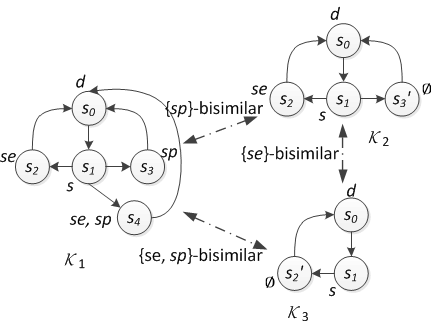
\includegraphics[width=8cm]{NVBnewCar.png}\\
  \caption{$V$-bisimulation between $\MPK$-structures}\label{v1uv2}
\end{figure}

%\textcolor{blue}{Let ${\cal K}_1$, ${\cal K}_2$ be two initial \MPK-structures described in Figure~\ref{yBisim}. It is easy to check ${\cal K}_1 \lrto_{\{y\}} {\cal K}_2$.}
% \begin{figure}[ht]
%   \centering
%   % Requires \usepackage{graphicx}
%   \includegraphics[width=8cm]{yBisim.png}\\
%   \caption{Two $\{y\}$-bisimular initial \MPK-structures}\label{yBisim}
% \end{figure}
\end{example}

%\textcolor{green}{It is  evident that $\lrto_V$ is a binary relation.}


When the underlying initial structures are clear from the context, we shall adopt the simplified notation $s_1 \lrto_V s_2$ emphasising states, to denote ${\cal K}_1 \lrto_V {\cal K}_2$.
 %In the sequel, we shall simplify the notation further and write $s_1 \lrto_V s_2 $ to denote ${\cal K}_1 \lrto_V {\cal K}_2$ whenever the underlying initial structures are clear from the context.

 % The next lemma easily follows from the above definition,
\begin{lemma}\label{lem:equive}
  The relation $\lrto_V$ is an equivalence relation.
\end{lemma}
%\begin{proof} See appendix. \end{proof}

Next, we give some further key properties of $\lrto_V$ w.r.t. different $V$s.
\begin{proposition}\label{div}
Let $i\in \{1,2\}$, $V_1,V_2\subseteq\cal A$, $s_1'$ and $s_2'$ be two states,
  $\pi_1'$ and $\pi_2'$ be two paths,
and ${\cal K}_i=({\cal M}_i,s_i)~(i=1,2,3)$ be \MPK-structures
 such that
${\cal K}_1\lrto_{V_1}{\cal K}_2$ and ${\cal K}_2\lrto_{V_2}{\cal K}_3$.
 Then:
 \begin{enumerate}[(i)]
   \item $s_1'\lrto_{V_i}s_2'~(i=1,2)$ implies $s_1'\lrto_{V_1\cup V_2}s_2'$;
   \item $\pi_1'\lrto_{V_i}\pi_2'~(i=1,2)$ implies $\pi_1'\lrto_{V_1\cup V_2}\pi_2'$;
   \item for each path $\pi_{s_1}$ of $\Hm_1$ there is a path $\pi_{s_2}$  of $\Hm_2$ such that $\pi_{s_1} \lrto_{V_1} \pi_{s_2}$, and vice versa;
   \item ${\cal K}_1\lrto_{V_1\cup V_2}{\cal K}_3$;
   \item If $V_1 \subseteq V_2$ then ${\cal K}_1 \lrto_{V_2} {\cal K}_2$.
 \end{enumerate}
\end{proposition}
% \begin{proof}
% We give proofs of (iii) and (iv) here. Proofs of other propositions can be found in the appendix.
% For convenience, we will refer to $\lrto_V$ by $\cal B$.

% (iii)
% %It is clear from Proposition~\ref{Vbi:Equ}.
% %\begin{proposition}\label{Vbi:Equ}
% The following property show our result directly.
% Let $V\subseteq\cal A$
% %${\cal M}_i=(S_i,R_i,L_i,s_0^i)~(i=1,2)$ be model structures
% and ${\cal K}_i=({\cal M}_i,s_i)~(i=1,2)$ be \MPK-structures.
% Then $({\cal K}_1,{\cal K}_2)\in\cal B$ if and only if
%   \begin{enumerate}[(a)]
%     \item $L_1(s_1)- V = L_2(s_2)- V$,
%     \item for every $(s_1,s_1')\in R_1$, there is $(s_2,s_2')\in R_2$
%     such that $({\cal K}_1',{\cal K}_2')\in \Hb$, and
%     \item for every $(s_2,s_2')\in R_2$, there is $(s_1,s_1')\in R_1$
%     such that $({\cal K}_1',{\cal K}_2')\in \Hb$,
%   \end{enumerate}
%  where ${\cal K}_i'=({\cal M}_i,s_i')$ with $i\in\{1,2\}$.

%  We prove it from the following two aspects:

%  $(\Rto)$
% (a) It is apparent that $L_1(s_1)- V = L_2(s_2)- V$;
% (b) %We will show that for each $(s_1, s_1') \in R_1$, there is a $(s_2, s_2')\in R_2$ such that $({\cal K}_1', {\cal K}_2') \in \Hb$.
% $({\cal K}_1, {\cal K}_2) \in \Hb$ iff $({\cal K}_1, {\cal K}_2) \in \Hb_i$ for all $i \geq 0$, then for each $(s_1, s_1') \in R_1$, there is a $(s_2, s_2')\in R_2$  such that  $({\cal K}_1', {\cal K}_2') \in \Hb_{i-1}$ for all $i > 0$ and then $L_1(s_1')- V = L_2(s_2')- V$. Therefore, $({\cal K}_1', {\cal K}_2') \in \Hb$.
% (c) %We will show that for each $(s_2, s_2') \in R_1$, there is a $(s_1, s_1')\in R_2$ such that $({\cal K}_1', {\cal K}_2') \in \Hb$.
%  This is similar with (b).

% $(\Lto)$ Apparently, $L_1(s_1)- V = L_2(s_2)- V$ implies that $(s_1, s_2) \in \Hb_0$;
%   (b) implies that for every $(s_1,s_1')\in R_1$, there is $(s_2,s_2')\in R_2$
%     such that $({\cal K}_1',{\cal K}_2')\in \Hb_i$ for all $i \geq 0$;
%   (c) implies that for every $(s_2,s_2')\in R_2$, there is $(s_1,s_1')\in R_1$
%     such that $({\cal K}_1',{\cal K}_2')\in \Hb_i$ for all $i \geq 0$.
% Hence, we have $({\cal K}_1, {\cal K}_2) \in \Hb_i$ for all $i \geq 0$,
% and then $({\cal K}_1,{\cal K}_2)\in\cal B$.
% %\end{proposition}


% (iv) Let ${\cal M}_i=(S_i,R_i,L_i,s_i)~(i=1,2,3)$, $s_1 \lrto_{V_1} s_2$ via a binary relation $\Hb$, and $s_2 \lrto_{V_2} s_3$ via a binary relation $\Hb''$. Let $\Hb' = \{(w_1, w_3)| (w_1, w_2)\in \Hb$ and $(w_2, w_3)\in \Hb_2\}$. It's apparent that $(s_1, s_3) \in \Hb'$. We prove $\Hb'$ is a $V_1 \cup V_2$-bisimulation relation containing $(s_1, s_3)$ from the (a), (b) and (c) of the previous step (iii) of $X$-bisimulation (where $X$ is a set of atoms). For all $(w_1, w_3) \in \Hb'$:
% \begin{enumerate}[(a)]
%   \item there exists $w_2 \in S_2$ such that $(w_1,w_2)\in \Hb$ and $(w_2, w_3)\in \Hb''$, and for all $q \notin V_1$, $q \in L_1(w_1)$ iff $q \in L_2(w_2)$ by $w_1 \lrto_{V_1} w_2$ and for all $q' \notin V_2$, $q'\in L_2(w_2)$ iff $q'\in L_3(w_3)$ by $w_2 \lrto_{V_2} w_3$. Then we have for all $r\notin V_1 \cup V_2$, $r \in L_1(w_1)$ iff $r \in L_3(w_3)$.
%   \item if $(w_1, u_1) \in \Hr_1$, then there exists $u_2\in S_2$ such that $(w_2, u_2) \in \Hr_2$ and $(u_1,u_2)\in \Hb$ (due to $(w_1,w_2)\in \Hb$ and $(w_2, w_3) \in \Hb''$ by the definition of $\Hb'$); and then there exists $u_3 \in S_3$ such that $(w_3, u_3) \in \Hr_3$ and $(u_2, u_3) \in \Hb''$, hence $(u_1, u_3) \in \Hb'$ by the definition of $\Hb'$.
%   \item if $(w_3, u_3) \in \Hr_3$, then there exists $u_2\in S_2$ such that $(w_2, u_2) \in \Hr_2$ and $(u_2, u_3) \in \Hb_2$; and then there exists $u_1 \in S_1$ such that $(w_1, u_1) \in \Hr_1$ and $(u_1, u_2) \in \Hb$, hence $(u_1, u_3) \in \Hb'$ by the definition of $\Hb'$.
% \end{enumerate}
% \end{proof}

In Proposition~\ref{div}, properties $(i)$ to $(iii)$ are the standard properties for $V$-bisimulation.
Property $(iv)$ shows that if a \MPK-structure is $V_1$ and $V_2$-bisimilar with the other two \MPK-structures, respectively, then those two \MPK-structures are $V_1 \cup V_2$-bisimilar. For an example, see Figure~\ref{v1uv2}. This property is crucial for forgetting.
%since it lays the foundation of forgetting atoms in $V$ one by one.
And last, $(v)$ says that if two \MPK-structures are  $V_1$-bisimilar, then they are $V_2$-bisimilar for any $V_2$ with $V_1\subseteq V_2 \subseteq \Ha$.





Intuitively, if two \MPK-structures are $V$-bisimilar, then they satisfy the same formula $\varphi$ that does not contain any atoms in $V$, i.e., $\IR(\varphi, V)$. This idea has been formalized and shown in the following theorem.

\begin{theorem}\label{thm:V-bisimulation:EQ}
  Let $V\subseteq\cal A$, ${\cal K}_i~(i=1,2)$ be two \MPK-structures such that
  ${\cal K}_1\lrto_V{\cal K}_2$ and $\phi$ be a formula with $\IR(\phi,V)$. Then
  ${\cal K}_1\models\phi$ if and only if ${\cal K}_2\models\phi$.
\end{theorem}

% \begin{proof}(sketch)
% This can be proved by induction on the structure of $\phi$. % and supposing $\Var(\phi) \cap V = \Empty$ due to $\IR(\phi,V)$.
% For instance, let $\phi = \psi_1 \vee \psi_2$, the induction hypothesis is ${\cal K}_1 \models \psi_i$ iff ${\cal K}_2 \models \psi_i$ with $i\in \{1,2\}$. Then we can see that ${\cal K}_1 \models \phi$ iff ${\cal K}_1 \models \psi_1$ or ${\cal K}_1 \models \psi_2$ iff ${\cal K}_2 \models \psi_1$ or ${\cal K}_2 \models \psi_2$ by induction hypothesis.
% %Other cases can be proved similarly.
% \end{proof}

Below, we illustrate this idea over an example.

\begin{example}[cont'd from Example~\ref{ex:2}]\label{ex:3}
Let $\varphi_1= d \wedge \EXIST\FUTURE se \wedge \ALL\GLOBAL(se \rto \ALL\NEXT d)$ and $\varphi_2= d \wedge \ALL \NEXT se$ be two \CTL\ formulae.  They are  $\{sp\}$-irrelevant. One can see that ${\cal K}_1$ and ${\cal K}_2$ in Figure~\ref{v1uv2} satisfy $\varphi_1$, but not $\varphi_2$.

%\textcolor{blue}{Let $\varphi_1= \neg p \wedge \ALL \NEXT q \wedge \EXIST \NEXT(x \rto \EXIST \NEXT x)$ and $\varphi_2 = q \wedge \ALL \NEXT q$ be two \CTL\ formulae.
% They are  $\{y\}$-irrelevant. One can check that ${\cal K}_1$ and ${\cal K}_2$ in Figure~\ref{yBisim} satisfy $\varphi_1$, but they do not satisfy $\varphi_2$.}
\end{example}
Next, we define the $V$-bisimulation between computation trees (of two initial structures). This construction will become useful when we define the characterizing formula of an initial $\MPK$-structure using the characterizing formula of a computation tree.


Let $V\subseteq\cal A$, ${\cal M}_i~(i=1,2)$ be  initial  structures.
A computation tree $\Tr_n(s_1)$ of ${\cal M}_1$ is $V$-{\em bisimilar}
to a computation tree $\Tr_n(s_2)$ of ${\cal M}_2$, written
$({\cal M}_1,\Tr_n(s_1))\lrto_V({\cal M}_2,\Tr_n(s_2))$ (or simply
$\Tr_n(s_1)\lrto_V\Tr_n(s_2)$), if % $({\cal M}_1,s_1)\lrto_V({\cal M}_2,s_2)$.
\begin{itemize}
  \item $L_1(s_1)- V=L_2(s_2)- V$,
  \item For every subtree $\Tr_{n-1}(s_i')$ of $\Tr_n(s_i)$,
  $\Tr_n(s_{(i \mod 2)+1})$ has a subtree $\Tr_{n-1}(s_{(i \mod 2)+1}')$ such that
  $\Tr_{n-1}(s_i')\lrto_V\Tr_{n-1}(s_{(i \mod 2)+1}')$.
 % \item for every subtree $\Tr_{n-1}(s_2')$ of $\Tr_n(s_2)$,
 %$\Tr_n(s_1)$ has a subtree $\Tr_{n-1}(s_1')$ such that
 %$\Tr_{n-1}(s_1')\lrto_V\Tr_{n-1}(s_2')$.
\end{itemize}
%Note that
The last condition in the above definition
hold trivially for $n=0$.

\begin{proposition}\label{B_to_T}
  Let $V\subseteq\cal A$ and $({\cal M}_i,s_i)~(i=1,2)$ be two \MPK-structures.
  Then
  \[(s_1,s_2)\in{\cal B}_n\mbox{ iff }
  \Tr_j(s_1)\lrto_V\Tr_j(s_2)\mbox{ for every $0\le j\le n$}.\]
\end{proposition}
% \begin{proof}(sketch)
% ($\Rto$) $\Tr_j(s_1)\lrto_V\Tr_j(s_2)$ for every $0\le j\le n$ is evident since $(s_1,s_2)\in{\cal B}_n$ implies that $(s_1,s_2)\in{\cal B}_j$ for every $0 \le j \le n$.

% ($\Lto$) In order to show $(s_1,s_2)\in{\cal B}_n$ we need only to prove for any $s_1'$ with $(s_1, s_1') \in R_1$ there is $s_2'$ with $(s_2, s_2')\in R_2$ s.t. $(s_2, s_2') \in {\cal B}_{n-1}$ and vice versa.
% $\Tr_0(s_1)\lrto_V\Tr_0(s_2)$ implies $(s_1, s_2) \in B_0$, $\Tr_1(s_1)\lrto_V\Tr_1(s_2)$ implies for any $s_1'$ with $(s_1, s_1') \in R_1$ there is $s_2'$ with $(s_2, s_2')\in R_2$ s.t. $(s_2, s_2') \in B_0$ and vice versa, hence $(s_1, s_2) \in B_1$. Therefore, we can prove $(s_1,s_2)\in{\cal B}_n$ recursively.
% \end{proof}
Proposition~\ref{B_to_T} says that a state $s_1$ of an initial structure is $V$-bisimilar to a state $s_2$ of another initial structure at a particular depth $n$ if, and only if,  all of the respective sub-trees rooted at $s_1$ and $s_2$ until depth $n$ are $V$-bisimilar.


%This means that $\Tr_j(s_1) \lrto_V \Tr_j(s_2)$ for all $j \geq 0$ if $s_1 \lrto_V s_2$, otherwise there is some $k$ such that $\Tr_k(s_1)$ and $\Tr_k(s_2)$ are not $V$-bisimilar.
Moreover, if two states $s$ and $s'$ from the same initial structure are not $V$-bisimilar, then the computation trees rooted at $s$ and $s'$, respectively, are not $V$-bisimilar at some depth  $k\in \mathbb{N}$. This is shown in the following proposition.

\begin{proposition}\label{pro:k}
  Let $V\subseteq \Ha$, $\Hm$ be an initial  structure and $s,s'\in S$
  such that $s\not\lrto_V s'$.
  There exists a least $k$ such that
  $\Tr_k(s)$ and $\Tr_k(s')$ are not $V$-bisimilar.
\end{proposition}
% \begin{proof}
% If $s\not\lrto_V s'$, then there exists a least constant $c$ such that $(s_i, s_j) \notin \Hb_c$, and then there is a least constant $m$ ($m \leq c$) such that $\Tr_m(s_i)$ and $\Tr_m(s_j)$ are not V-bisimilar by Proposition~\ref{B_to_T}. Let $k=m$, the lemma is proved.
% \end{proof}

%We will say that two states $s$ and $s'$ in $\Hm$ are $V$-distinguishable, if there exists a least constant $k$ such that $\Tr_k(s) \not \lrto_{\overline V} \Tr_k(s')$, which is denoted by $\dis_V({\cal M},s,s',k)$. We call an initial  structure ${\cal M}$ is $V$-{\em distinguishable} if there are two states $s$ and $s'$ in $\Hm$ such that $s$ and $s'$ are $V$-distinguishable.


% We will say that two states $s$ and $s'$ in $\Hm$ are $V$-{\em distinguishable}, if there exists $k \in \mathbb{N}$ such that $\Tr_k(s) \not \lrto_{\overline V} \Tr_k(s')$, and write that $\dis_V({\cal M},s,s',k)$. For convenience, we will assume the smallest number. Furthermore, we say that an initial  structure ${\cal M}$ is $V$-{\em distinguishable} if there are two states $s$ and $s'$ in $\Hm$ such that $s$ and $s'$ are $V$-distinguishable.

%\textcolor{blue}{In this case, the  initial  structure ${\cal M}$ is called $V$-{\em distinguishable} (by
%states $s$ and $s'$ at the least depth $k$), which is denoted by $\dis_V({\cal M},s,s',k)$.}
%It is evident that
%$\dis_V({\cal M},s,s',k)$ implies $\dis_V({\cal M},s,s',k')$ whenever $k'\ge k$.
% The $V$-{\em characterization number}
% of ${\cal M}$, written $ch({\cal M},V)$, is defined as
% \[ch({\cal M},V)=
% \left\{
%   \begin{array}{ll}
%     \max\{k\mid s,s'\in S \text{ and }\dis_V({\cal M},s,s',k)\},\\
%          \ \ \qquad \qquad \qquad \hbox{${\cal M}$ is $V$-distinguishable;} \\
%     \min\{k\mid {\cal B}_{k}={\cal B}_{k+1}\}, \ \ \ \quad \qquad \hbox{otherwise.}
%   \end{array}
% \right.
% \]
% \textcolor{red}{We can see that the $ch(\Hm, V)$ always exists for every initial  structure $\Hm$ and $V\subseteq \Ha$: if there are two states $s_1$ and $s_2$ such that $s_1$ and $s_2$ are $V$-distinguishable, then the characterization number exists by the definition of $ch({\cal M},V)$; else, we have that for each $s, s’$ in $\Hm$, $((\Hm,s), (\Hm, s’)) \in \Hb_k$ for all $k \geq 0$ and then there exists a least number $n \in \mathbb{N}$ such that $\Hb_n = \Hb_{n+1}$ since the set of states in $\Hm$ is finite.
% Intuitively, given a state $s$ in $\Hm$, the $V$-characterization number $c$ of $\Hm$ is used to divide the states in $\Hm$ into two classes, one contains those states $s’$ that $(\Hm,s’) \models \varphi_c$ and the other one contains other states, where $\varphi_c$ is a characterizing formula, which will be given in the next subsection, of the computation tree $\Tr_c(s)$. }

\subsection{Characterization of an Initial \MPK-structure}
% \textcolor{red}{Inspired by the Hintikka formulae, \dots. The computation tree with depth $n\in \mathbb{N}$ and the initial $\MPK$-structure can be captured by \CTL\ formulas respectively.}

In the following, we present characterizing formulas of initial \MPK-structures  over a signature to characterize the $\lrto_V$-class of an initial \MPK-structure.
\footnote{Similar approaches has been taken in the literature e.g., in~\cite{DBLP:conf/birthday/1997ehrenfeucht},  a class (namely, $\equiv_{\overline{k}}$-class) of structures of monadic formulas has been characterized by Hintikka formulae~\cite{hintikka1953distributive}. Another example is Yankov-Fine construction in \cite{yankov1968three}.}


To start with, we give the definition of characterizing formulas of computation trees.
\begin{definition}\label{def:V:char:formula}
Let $V\subseteq \Ha$, $\Hm =(S,R,L,s_0)$ be an initial structure and $s\in S$.
The {\em characterizing formula} of the computation tree $\Tr_n(s)$ on $V$,
written ${\cal F}_V(\Tr_n(s))$, is defined recursively as:
\begin{align*}
   {\cal F}_V(\Tr_0(s)) &=  \bigwedge_{p \in V\cap L(s)}p
     \wedge \bigwedge_{q\in V-L(s)} \neg q,\\
   {\cal F}_V(\Tr_{k+1}(s))& = \bigwedge_{(s,s')\in R}
    \EXIST \NEXT {\cal F}_V(\Tr_k(s'))\\
  \wedge &
    \ALL \NEXT \left( \bigvee_{(s,s')\in R} {\cal F}_V(\Tr_k(s')) \right) \wedge {\cal F}_V(\Tr_0(s))
\end{align*}
for $k\ge 0$.
\end{definition}
The characterizing formula of a computation tree formally exhibits the content of each node in $V$ (i.e., atoms in $V$ that are {\em true}  if they are in the label of this node of the computation tree, and {\em false} otherwise) and the temporal relation between states recursively.
Clearly, ${\cal F}_V(\Tr_0(s))$ expresses the content of node $s$ in terms of $V$, the conjunction with $\EXIST \NEXT$ part guarantees that each direct successor $s'$ of $s$ is captured by a \CTL\ formula until depth $k$, and the $\ALL \NEXT$ part guarantees that for each direct successor $s'$ of $s$ there exists another direct successor $s''$ of $s$ such that $s''$ is $V$-bisimilar to $s'$ until depth $k$.

The following result shows that the $V$-bisimulation between two computation trees implies the semantic equivalence of the corresponding characterizing formulas.

\begin{lemma}\label{lem:Vb:TrFormula:Equ}
Let $V\subseteq \Ha$, and $\Hm, \Hm'$ be two initial structures,
$s\in S$, $s'\in S'$ and $n\ge 0$. If $\Tr_n(s) \lrto_{\overline V} \Tr_n(s')$, then ${\cal F}_V(\Tr_n(s)) \equiv {\cal F}_V(\Tr_n(s'))$.
\end{lemma}
% \begin{proof}(sketch)
% This result can be proved by induction on $n$.

% For the base. It is evident that for any $s\in S$ and $s' \in S'$, if $\Tr_0(s) \lrto_{\overline V} \Tr_0(s')$ then ${\cal F}_V(\Tr_0(s)) \equiv {\cal F}_V(\Tr_0(s'))$ due to $L(s) - \overline V = L'(s') - \overline V$ by the definition of the $V$-bisimulation.

% For the induction step. If $\Tr_n(s) \lrto_{\overline V} \Tr_n(s')$ we can prove for each state $s_1$ with $(s,s_1)\in R$ there is $s_1'$ with $(s',s_1')\in R'$ such that ${\cal F}_V(\Tr_n(s_1)) \equiv {\cal F}_V(\Tr_n(s_1'))$ and vice versa. Then it is easy check ${\cal F}_V(\Tr_n(s)) \equiv {\cal F}_V(\Tr_n(s'))$.
% \end{proof}
In Lemma~\ref{lem:Vb:TrFormula:Equ}, let $s'=s$. Then, it is easy to see that for any formula $\varphi$ of $V$, if $\varphi$ is a characterizing formula of $\Tr_n(s)$ then $\varphi \equiv {\cal F}_V(\Tr_n(s))$.


The notion of $V$-bisimulation and Proposition~\ref{pro:k} naturally induce a complementary notion, so-called $V$-\emph{distinguishability}, which will turn out to be useful in defining the characterizing formula of an initial \MPK-structure.
In particular, we will say that two states $s$ and $s'$ of $\Hm$ in Proposition~\ref{pro:k} are $V$-{\em distinguishable} if $s \not \lrto_{\overline V} s'$, and write that $\dis_V({\cal M},s,s',k)$, where we assume $k$ to be the  smallest natural number which makes $s$ and $s'$ $V$-distinguishable. Furthermore, we say that an initial  structure ${\cal M}$ is $V$-distinguishable if there are two states $s$ and $s'$ in $\Hm$ that are $V$-distinguishable. Then given an initial structure $\mathcal{M}$ and a set $V$ of atoms, the smallest value of $k$ which ensures $V$-distinguishability  is in question. We shall call such a $k$ as the \emph{characterization number} of $\mathcal{M}$ w.r.t. $V$ and define it formally as
%\textcolor{red}{Now in defining the characterizing formula of an initial \MPK-structure $\Hm$ on $V$, we will need to use the notion of $V$-bisimilar up to a certain degree,} that is,
\[ch({\cal M},V)=
\left\{
  \begin{array}{ll}
    \max\{k\mid s,s'\in S \text{ and }\dis_V({\cal M},s,s',k)\},\\
         \ \ \qquad \qquad \qquad \hbox{${\cal M}$ is $V$-distinguishable;} \\
    \min\{k\mid {\cal B}_{k}={\cal B}_{k+1}\}, \ \ \ \quad \qquad \hbox{otherwise.}
  \end{array}
\right.
\]
 since it will be crucial in defining the characterization formula (for a given initial $\MPK$-structure).

Observe that the $ch(\Hm, V)$ always exists for every initial  structure $\Hm$ and $V\subseteq \Ha$: If there are two states $s_1$ and $s_2$ such that $s_1$ and $s_2$ are $V$-distinguishable, then the characterization number exists by definition. In the extreme case, if for all $s, s'$ in $\Hm$, $((\Hm,s), (\Hm, s')) \in \Hb_k$ for all $k \geq 0$, and  $\Hb_k = \Hb_{k+1}$ (since the set of states in $\Hm$ is always finite), then the characterization number is 0.

%if there are two states $s_1$ and $s_2$ such that $s_1$ and $s_2$ are $V$-distinguishable, then the characterization number exists by the definition of $ch({\cal M},V)$; else, we have that for each $s, s’$ in $\Hm$, $((\Hm,s), (\Hm, s’)) \in \Hb_k$ for all $k \geq 0$ and then there exists a least number $n \in \mathbb{N}$ such that $\Hb_n = \Hb_{n+1}$ since the set of states in $\Hm$ is finite.\\


%In fact, given a $\Hm$, if $\Hm$ is $V$-distinguishable then there must be a $k$ such that for any two $V$-distinguishble states $s$ and $s'$ in $\Hm$, we have $Tr_k(s) \not \lrto_{\overline V} Tr_k(s')$.\\

Intuitively, given a state $s \in S$ of $\Hm$, the characterization number $c$ of $\Hm$ divides the states in $\Hm$ into two classes: The one which contains those states $s'$ until depth $c$ such that $(\Hm,s') \models {\cal F}_V(\Tr_c(s))$, and the other which contains the remaining states. Now, we are finally ready to define the characterizing formula of an  initial \MPK-structure.
%, where $\varphi_c$ is a characterizing formula, which will be given in the next subsection, of the computation tree $\Tr_c(s)$. }
\begin{definition}[Characterizing Formula]
Let $V\subseteq\cal A$,
%, ${\cal M}=(S,R,L,s_0)$
 and ${\cal K}=({\cal M},s_0)$ be an initial \MPK-structure with $c=ch({\cal M},V)$, and for every state $s' \in S$ of $\Hm$, $T(s') = {\cal F}_V(\Tr_c(s'))$.
Then, the {\em characterizing formula} ${\cal F}_V({\cal K})$ of $\cal K$ on $V$ is:
\begin{align*}
  &T(s_0) \text{ } \wedge \\
  & \bigwedge_{s\in S}\ALL \GLOBAL\left(
    %{\cal F}_V(\Tr_c(s)) \rto
    T(s) \rto
    \bigwedge_{(s,s')\in R}
        \EXIST \NEXT T(s')
        \wedge
        \ALL \NEXT (\bigvee_{(s,s')\in R}T(s'))
    \right)
\end{align*}
%\begin{equation*}
%\resizebox{.91\linewidth}{!}{$
%    \displaystyle
%   \ALL \GLOBAL\left(
%    {\cal F}_V(\Tr_c(s)) \rto
%    \bigwedge_{(s,s')\in R}
%        \EXIST \NEXT T(s')
%        \wedge
%        \ALL \NEXT \bigvee_{(s,s')\in R}T(s')
%    \right)
%$}
%\end{equation*}
\end{definition}
Here, $T(s_0)$ ensures that the \MPK-structure starts from the initial state, and the remaining part ensures that we go deep enough in the computation tree (i.e., through all possible transitions from every state $s \in S$)  to detect any two  $V$-distinguishable states $s$ and $s'$ (which would then imply  $T(s) \not \equiv T(s')$). As a remark on notation, sometimes  we shall need to express the initial structure and the initial state explicitly, then we will use the rather transparent notation i.e., ${\cal F}_V(\Hm, s_0)$ (instead of ${\cal F}_V({\cal K})$).  %(or it expresses the initial state in the initial $\MPK$-structure),
%the $\bigwedge_{s\in S} \ALL \GLOBAL$ part describes all of the possible transitions from $s$ and each $T(s)$ ensures that we have explored the computation tree deep enough so that for any other $s'\in S$, if $s\not \lrto_{\overline V} s'$ (or $s$ and $s'$ are $V$-distinguishable) we have $T(s) \not \equiv T(s')$.}


One can observe that $\IR({\cal F}_V(\Hm, s_0), \overline V)$.
Besides, given a set of atomic propositions $V$, any initial \MPK-structure has its own unique characterizing formula on $V$. As we will see later, the characterizing formula will play a crucial role in showing important properties of forgetting, as well as in our main contribution which is  computing the SNC and WSC of a \CTL\ formula under an initial \MPK-structure.


% (2) It seems that this characterizing formula of an initial \MPK-structure rebuilt a new initial \MPK-structure: in which each node can be labeled as $T(s)$ with the $s$ is the corresponding node,  }

The following example illustrates how one can compute a characterizing formula:
\begin{example}[cont'd from Example~\ref{ex:2}]\label{ex:4}
%\textcolor{red}{(1) Consider the ${\cal K}_3 = (\Hm, s_0)$ from Figure~\ref{v1uv2}, its' computation trees rooted at $s_0$ with depth $0$, $1$, $2$ and $3$ respectively are in Figure~\ref{fig:CarcomTree} (the labels of the nodes in the trees are omitted for simplicity), let $V=\{d\}$ then $\overline{V}=\{s\}$. We can check that $\Tr_0(s_1) \lrto_{\overline{V}} \Tr_0(s_2)$ due to $L(s_1) - \overline{V} = L(s_2) - \overline{V}$ and $\Tr_1(s_1) \not \lrto_{\overline{V}} \Tr_1(s_2)$ since there is $(s_1, s_2)\in R$ such that for any $(s_2, s') \in R$ there is $L(s_2)- \overline V \neq L(s') - \overline V$ (there is only one immediate successor $s'=s_0$), hence we have $s_1$ and $s_2$ is $V$-distinguishable and  $\dis_{V}(\Hm, s_1, s_2, 1)$. Similarly, we have  $\dis_{ V}(\Hm, s_0, s_1, 0)$ and $\dis_{ V}(\Hm, s_0, s_2, 0)$. Therefore, $ch({\cal K}_3)=\max\{k\mid s,s'\in S \text{ and } \dis_{V}({\cal M},s,s',k)\} = 1$.
%Then we have:
%\begin{align*}
 %  {\cal F}_V(\Tr_0(s_0)) &= d, \\
  % {\cal F}_V(\Tr_0(s_1)) &= \neg d, \\
  % {\cal F}_V(\Tr_0(s_2)) &= \neg d, \\
  % {\cal F}_V(\Tr_1(s_0)) &= \EXIST\NEXT \neg d \wedge \ALL\NEXT \neg d \wedge d %\equiv \ALL\NEXT \neg d \wedge d, \\
 %  {\cal F}_V(\Tr_1(s_1)) &= \EXIST\NEXT \neg d  \wedge \ALL\NEXT \neg d \wedge \neg %d \equiv \ALL\NEXT \neg d \wedge \neg d, \\
  % {\cal F}_V(\Tr_1(s_2)) &= \EXIST\NEXT d  \wedge \ALL\NEXT d \wedge \neg d \equiv %\ALL\NEXT d \wedge \neg d,\\
 % {\cal F}_V(\Hm, s_0)&\equiv \ALL\NEXT \neg d \wedge d \wedge \\
 % & \ALL \GLOBAL(\ALL\NEXT \neg d \wedge d \rto \ALL\NEXT(\ALL\NEXT \neg d \wedge %\neg d))\wedge \\
 % & \ALL \GLOBAL(\ALL\NEXT \neg d \wedge \neg d \rto \ALL\NEXT(\ALL\NEXT d \wedge %\neg d)) \wedge\\
 % & \ALL \GLOBAL(\ALL\NEXT d \wedge \neg d \rto \ALL\NEXT(\ALL\NEXT \neg d \wedge %d)).
%\end{align*}}
%\begin{figure}
%  \centering
  % Requires \usepackage{graphicx}
 % \includegraphics[width=8.5cm]{CarCtree.png}
 % \caption{Computation trees rooted at $s_0$}\label{fig:CarcomTree}
%\end{figure}

Reconsider the ${\cal K}_2= (\Hm, s_0)$  in Figure~\ref{fig:K2Tree}, illustrated on the left side   (originally introduced in Figure~\ref{v1uv2}).   The corresponding computation trees are listed on the right side: from left to right, they are rooted at $s_0$ with depth $0$, $1$, $2$ and $3$, respectively. For simplicity, the labels of the nodes in the trees are omitted (See Figure~\ref{v1uv2} for the actual labels). Let $V=\{d\}$ then $\overline{V}=\{s, se\}$.

 We can see that $\Tr_0(s_1) \lrto_{\overline{V}} \Tr_0(s_2)$, since $L(s_1) - \overline{V} = L(s_2) - \overline{V}$. Moreover, $\Tr_1(s_1) \not \lrto_{\overline{V}} \Tr_1(s_2)$, since there is $(s_1, s_2)\in R$ such that for any $(s_2, s') \in R$, it is the case that $L(s_2)- \overline V \neq L(s') - \overline V$ (because there is only one direct successor $s'=s_0$). Hence, we have $s_1$ and $s_2$ which are $V$-distinguishable and  $\dis_{V}(\Hm, s_1, s_2, 1)$. Similarly, we have  $\dis_{ V}(\Hm, s_0, s_1, 0)$, $\dis_{V}(\Hm, s_0, s_2, 0)$ and $\dis_{ V}(\Hm, s_0, s_3', 0)$. Furthermore, we can see that $s_2 \lrto_{\overline V} s_3'$. Therefore, $ch(\Hm, V)=\max\{k\mid s,s'\in S \text{ and } \dis_{V}({\cal M},s,s',k)\} = 1$.
 And  we have the following:
 \begin{align*}
   {\cal F}_V(\Tr_0(s_0)) &= d, \qquad \quad {\cal F}_V(\Tr_0(s_1)) = \neg d, \\
   {\cal F}_V(\Tr_0(s_2)) &= \neg d,  \qquad  {\cal F}_V(\Tr_0(s_3')) = \neg d,\\
   {\cal F}_V(\Tr_1(s_0)) &= \EXIST\NEXT \neg d \wedge \ALL\NEXT \neg d \wedge d \equiv \ALL\NEXT \neg d \wedge d, \\
   {\cal F}_V(\Tr_1(s_1)) &= \EXIST\NEXT \neg d \wedge \EXIST\NEXT \neg d  \wedge \ALL\NEXT (\neg d \vee \neg d) \wedge \neg d \\
   &\equiv \ALL\NEXT \neg d \wedge \neg d, \\
   {\cal F}_V(\Tr_1(s_2)) &= \EXIST\NEXT d  \wedge \ALL\NEXT d \wedge \neg d \equiv \ALL\NEXT d \wedge \neg d,\\
   {\cal F}_V(\Tr_1(s_3')) &\equiv {\cal F}_V(\Tr_1(s_2)),\\
  {\cal F}_V(\Hm, s_0)&\equiv \ALL\NEXT \neg d \wedge d \wedge \\
  & \ALL \GLOBAL(\ALL\NEXT \neg d \wedge d \rto \ALL\NEXT(\ALL\NEXT \neg d \wedge \neg d))\wedge \\
  & \ALL \GLOBAL(\ALL\NEXT \neg d \wedge \neg d \rto \ALL\NEXT(\ALL\NEXT d \wedge \neg d)) \wedge\\
  & \ALL \GLOBAL(\ALL\NEXT d \wedge \neg d \rto \ALL\NEXT(\ALL\NEXT \neg d \wedge d)).
\end{align*}



 \begin{figure}
  \centering
  % Requires \usepackage{graphicx}
  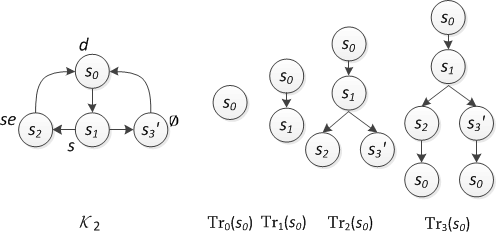
\includegraphics[width=8.5cm]{NK2Tree1.png}
  \caption{On the left side,  $\mathcal{K}_2$ (aforementioned in Figure~~\ref{v1uv2}), and on the right side, the corresponding computation trees of depth 0, 1, 2 and 3, respectively. Labels of the nodes are omitted for simplicity.}\label{fig:K2Tree}
\end{figure}
%Let ${\cal K} = (\Hm, s_0)$ with $\Hm=(S, R, L,s_0)$ be a initial \MPK-structure, % (in Fig.~\ref{Kripke_1}),
% in which $S=\{s_0, s_1, s_2\}$, $R=\{(s_0, s_1), (s_0, s_2), (s_1, s_0), (s_2, s_0)\}$, $L(s_0)= \{a\}$, $L(s_1) =\{a,c\}$ and $L(s_2) = \{b,c\}$. Let $V=\{a, b\}$, compute the characterizing formula of ${\cal K}$ on $V$.
%(2) Let ${\cal K} = (\Hm, s_0)$ in Figure~\ref{Kripke_1}, its' computation trees rooted at $s_0$ with depth $0$, $1$ and $2$ respectively are in Figure~\ref{fig:comTree} (the labels of the nodes in the trees are omitted for simplicity), be an initial \MPK-structure with initial state $s_0$ and $V=\{a, b\}$. It is evident that $\Tr_0(s_0) \lrto_{\overline V} \Tr_0(s_1)$ due to $L(s_0) - \overline V = L(s_1) - \overline V$, and $\Tr_1(s_0) \not\lrto_{\overline V} \Tr_1(s_1)$ since there is $(s_0, s_2)\in R$ such that for any $(s_1, s') \in R$ there is $L(s_2)- \overline V \neq L(s') - \overline V$ (there is only one immediate successor $s'=s_0$). Hence, we have that $\Hm$ is $V$-distinguishable and  $\dis_{V}(\Hm, s_0, s_1, 1)$. Similarly, we have $\dis_{ V}(\Hm, s_0, s_2, 0)$ and $\dis_{ V}(\Hm, s_1, s_2, 0)$. Therefore, $ch(\Hm, V) =  \max\{k\mid s,s'\in S \text{ and } \dis_{V}({\cal M},s,s',k)\} = 1$.
%It is apparent that $\Hb_0=\{(s_0, s_1)\}$ and $\Hb_1={\Empty}$, then $ch(\Hm, s_0) = 1$.
%Then we have:
%\begin{align*}
%  & {\cal F}_V(\Tr_0(s_0)) = a \wedge \neg b, \\
 % & {\cal F}_V(\Tr_0(s_1)) = a \wedge \neg b, \\
 %& {\cal F}_V(\Tr_0(s_2)) = b \wedge \neg a, \\
  %& {\cal F}_V(\Tr_1(s_0)) = \EXIST\NEXT(a \wedge \neg b)  \wedge \EXIST\NEXT(b %\wedge \neg a) \wedge \ALL\NEXT((a \wedge \neg b) \vee\\
  %& \qquad \qquad  \qquad (b \wedge \neg a)) \wedge (a \wedge \neg b), \\
  %& {\cal F}_V(\Tr_1(s_1)) = \EXIST\NEXT(a \wedge \neg b)  \wedge \ALL\NEXT(a \wedge \neg b) \wedge (a \wedge \neg b), \\
  %& {\cal F}_V(\Tr_1(s_2)) = \EXIST\NEXT(a \wedge \neg b)  \wedge \ALL\NEXT(a %\wedge \neg b) \wedge (b \wedge \neg a).
 %&{\cal F}_V(\Hm, s_0)= {\cal F}_V(\Tr_1(s_0)) \wedge  \bigwedge_{s\in S} \ALL \GLOBAL \left(
%  {\cal F}_V(\Tr_1(s)) \rto
%  \bigwedge_{(s,s')\in R}
%        \EXIST \NEXT {\cal F}_V(\Tr_1(s'))
%        \wedge
%        \ALL \NEXT \bigvee_{(s,s')\in R}{\cal F}_V(\Tr_1(s'))
%  \right)
%\end{align*}
 %Then it is easy to obtain ${\cal F}_V({\cal K})$ by the definition of the characterizing formula of ${\cal K}$ on $V$.}


%\begin{figure}
 % \centering
  % Requires \usepackage{graphicx}
  %\includegraphics[width=4cm]{kk1.png}\\
  %\caption{A simple initial structure}\label{Kripke_1}
%\end{figure}

%\begin{figure}
 % \centering
  % Requires \usepackage{graphicx}
 % \includegraphics[width=6cm]{Ctree.png}\\
 % \caption{Computation trees rooted at $s_0$}\label{fig:comTree}
%\end{figure}

%\textcolor{blue}{Let $V=\{sr\}$, $\overline V=\{sl,se,lc,le\}$ ($\Ha =\overline V\cup \{sr\}$), and $\Hm$ is as illustrated in Figure~1.  We have $\Tr_0(s_0) \not \lrto_{\overline V} \Tr_0(s_1)$ and $\Tr_0(s_0) \not \lrto_{\overline V} \Tr_0(s_2)$, then $\dis_{\overline V}(\Hm, s_0, s_1, 0)$ and $\dis_{\overline V}(\Hm, s_0, s_2, 0)$.
%Besides, it is easy to check that $s_1 \lrto_{\overline V} s_2$ since they have the %same direct successor $s_0$.
%Hence, $ch(\Hm, V) = 0$.
%Therefore, %we have:
%\begin{align*}
%& {\cal F}_V(\Tr_0(s_0))= \neg sr \\
%& {\cal F}_V(\Tr_0(s_1)) = {\cal F}_V(\Tr_0(s_2)) = sr, \text{ and  }\\
%\end{align*}
%Then we have,
%\begin{align*}
%& {\cal F}_V (\Hm, s_0)\textcolor{red}{\equiv} \neg sr \wedge \ALL\GLOBAL(\neg sr \rto  \ALL \NEXT sr)\wedge \ALL\GLOBAL(sr \rto  \ALL \NEXT \neg sr).
%\end{align*}}

\end{example}


The following result shows that there is a correspondence between the semantic equivalence of characterizing formulae and the initial \MPK-structures which are $V$-bisimilar. That is, two initial \MPK-structures are $V$-bisimilar if, and only if  their characterizing formulae are semantically equivalent. This means,  characterizing formula characterizes initial \MPK-structures which are equivalent up to $V$-bisimulation.

%characterizing formulae of an initial \MPK-structure are equivalent and \textcolor{red}{the characterizing formula of an initial \MPK-structure characterizes that initial \MPK-structure up to $V$-bisimulation}.


\begin{theorem}\label{CF}
Let $V\subseteq \Ha$, $\Hm=(S,R,L,s_0)$ and $\Hm'=(S',R', L',s_0')$ be two initial structures. Then,
\begin{enumerate}[(i)]
 \item $(\Hm',s_0') \models {\cal F}_V({\cal M},s_0)
\text{ iff }
({\cal M},s_0) \lrto_{\overline V} ({\cal M}',s_0')$;

\item $s_0 \lrto_{\overline V} s_0'$ implies  ${\cal F}_V(\Hm, s_0) \equiv {\cal F}_V(\Hm', s_0')$.
\end{enumerate}

\end{theorem}
% \begin{proof} (sketch)
%  Let $c={ch({\cal M},V)}$, %we give the proof idea of it.
% On the one hand, one can verify that $({\cal M},s)\models{\cal F}_V(\Tr_n(s))$ holds for $n \geq 0$, which implies $(\Hm, s)\models {\cal F}_V(\Tr_c(s))$.
% On the other hand, $({\cal M},s)\models{\cal F}_V(\Tr_n(s'))$ implies
%   $\Tr_n(s) \lrto_{\overline V} \Tr_n(s')$. In this case, it is not difficult to see that for each $s'\in S$, $({\cal M},s) \lrto_{\overline V} ({\cal M},s')$ if and only if $({\cal M},s')\models{\cal F}_V(\Tr_c(s))$. %And then obtained our result.

%  (i) ($\Lto$) This is evident due to $(\Hm, s_0) \models {\cal F}_V(\Hm, s_0)$ and $\IR({\cal F}_V(\Hm, s_0), \overline V)$, hence $(\Hm',s_0') \models {\cal F}_V(M,s_0)$ by Theorem~\ref{thm:V-bisimulation:EQ}.

% ($\Rto$) We can prove this by showing that for all $n \geq 0$, $Tr_n(s_0) \lrto_{\overline V} Tr_n(s_0')$ by Proposition~\ref{B_to_T}. The base case, \ie $n=0$, is easy. A key point for  the  induction  step is that $(\Hm',s_0') \models {\cal F}_V(\Hm,s_0)$
%       implies for all $s'\in S'$, $(\Hm', s')\models {\cal F}_V(\Tr_c(s)) \rto$  $\left(\bigwedge_{(s,s_1)\in R} \EXIST \NEXT {\cal F}_V(\Tr_c(s_1))\right)\wedge \ALL \NEXT \left( \bigvee_{(s,s_1)\in R} {\cal F}_V(\Tr_c(s_1))\right)$  for any $s\in S$.
% For further details, please see the supplementary material.

% (ii) This is implied by Lemma~\ref{lem:Vb:TrFormula:Equ}.
% \end{proof}

% \textcolor{red}{Theorem~\ref{CF} means that the characterizing formula of an initial \MPK-structure characterizes that initial \MPK-structure up to $V$-bisimulation.}





It is noteworthy that under our assumption of bounded size (of a \CTL\ formula), say $n$, it will be sufficient to consider the models of formulas within a state space $S$ satisfying $|S|=n8^n$~\cite{DBLP:journals/jcss/EmersonH85}.
%Recall that under the bounded \CTL\ assumption every formula has bounded length, say $n$. It is sufficient to consider the models of formulas within a state space $S$ satisfying $|S|=n*(8^n)$~\cite{DBLP:journals/jcss/EmersonH85}.
Any other model must be bisimilar to some model within the state space, and their characterizing formulas are equivalent due to Theorem~\ref{CF}. Therefore, given a formula of size within the bound, only a finite number of such initial \MPK-structures need to be considered as the candidate models. This fact is expressed in the following lemma.
%\textcolor{blue}{Recall that the number of initial structures is finite.
%The next lemma is evident in terms of the above theorem.}
\begin{lemma}\label{lem:models:formula}
  Let $\varphi$ be a formula. We have
  \begin{equation}
    \varphi\equiv \bigvee_{(\Hm, s_0)\in\Mod(\varphi)}{\cal F}_{\cal A}(\Hm, s_0).
\end{equation}
\end{lemma}
Yet Lemma~\ref{lem:models:formula} has an additional message: Any \CTL\ formula  can be expressed in the form of a disjunction of the characterizing formulae of its models. This fact will be  crucial  in the results we present in next sections.

\subsection{Semantic Properties of Forgetting in \CTL}
In this subsection, we present the notion of forgetting in \CTL\ and investigate its semantic properties. Let us start with the formal definition.
%\textcolor{red}{Based on our notion of $V$-bisimulation, we can now introduce forgetting in \CTL\ from the semantic forgetting point view.
%Which means the result of forgetting the atoms in set $V$ of atoms from \CTL\ formula $\varphi$ is a formula which shares the same models as $\varphi$ and models that are $V$-bisimulation with one of the models of $\varphi$.}}
% We will first show via a representation theorem that our definition of forgetting correspond to the readily existing notion of forgetting which is characterised by several desirable properties (also called postulates) suggested in~\cite{Yan:AIJ:2009}. Next, we discuss various additional semantic properties of forgetting.
%
%Now, we give the formal definition of forgetting in \CTL\ from the semantic point view.
\begin{definition}[Forgetting]\label{def:V:forgetting}
  Let $V\subseteq\cal A$ and $\phi$ be a formula.
A formula $\psi$ with $\Var(\psi)\cap V=\emptyset$
is a {\em result of forgetting $V$ from} $\phi$ (denoted as $\CTLforget(\phi,V)$), if
\begin{equation*}
\resizebox{.91\linewidth}{!}{$
\displaystyle
  \Mod(\psi)=\{{\cal K}\mbox{ is initial}\mid \exists {\cal K}'\in\Mod(\phi)\ \text{ \st }\ {\cal K}'\lrto_V{\cal K}\}.
  $}
\end{equation*}
\end{definition}
Realize that Definition~\ref{def:V:forgetting} implies if both $\psi$ and $\psi'$ are results of forgetting $V$ from $\phi$, then
$\Mod(\psi)=\Mod(\psi')$, i.e., $\psi$ and $\psi'$ have the same models. In this sense, the result of  forgetting $V$ from $\phi$ is unique (up to semantic equivalence).
By Lemma~\ref{lem:models:formula}, such a formula always exists, which
is equivalent to
\begin{equation*}
  \bigvee_{{\cal K}\in  \{{\cal K}'\mid \exists {\cal K}''\in\Mod(\phi)\ \text{ and }\ {\cal K}''\lrto_V{\cal K}'\}} {\cal F}_{\overline V}({\cal K}).
\end{equation*}
%For this reason,
At this point, it is important to emphasize that, the notion of forgetting  we have defined for \CTL\ respects the classical forgetting defined for propositional logic (PL)~\cite{lin1994forget}. To see this, assume that $\varphi$ is a PL formula and $p\in \Ha$, then $\Forget(\varphi, p)$ is a result of forgetting $p$ from $\varphi$; that is, $\Forget(\varphi, p)\equiv \varphi[p/\bot] \vee \varphi[p/\top]$.
% , where $\varphi[p/\bot]$ and $\varphi[p/\top]$ denote the formulae obtained from $\varphi$ by replacing atom $p$ with $\bot$ and $\top$, respectively.
That way, given a set $V\subseteq \Ha$, one can recursively define $\Forget(\varphi, V\cup \{p\}) = \Forget(\Forget(\varphi, p),V)$, where $\Forget(\varphi, \emptyset) = \varphi$. Using this insight, the following result shows that the classical notion of forgetting (for PL ~\cite{lin1994forget}) is a special case of forgetting in CTL.


\begin{theorem}\label{thm:PL:CTL}
Let $\varphi$ be a PL formula and $V\subseteq \Ha$, then
\[
\CTLforget(\varphi, V) \equiv \Forget(\varphi, V).
\]
\end{theorem}

In~\cite{Yan:AIJ:2009}, authors give four postulates concerning knowledge forgetting in  \SFive\ modal logic (also called \emph{forgetting postulates}) which can be  considered as desirable properties of such a notion. In the following, we first list these postulates, and then show that our notion of forgetting in \CTL\ satisfies them.

\textbf{Forgetting postulates}~\cite{Yan:AIJ:2009} are:
\begin{itemize}
  \item[] (\W) Weakening: $\varphi \models \varphi'$;
  \item[] (\PP) Positive Persistence:
  for any formula $\eta$, if $\IR(\eta, V)$ and $\varphi \models \eta$ then $\varphi' \models \eta$;
  \item[] (\NgP) Negative Persistence :  for any formula $\eta$,  if $\IR(\eta, V)$ and $\varphi \not \models \eta$ then $\varphi' \not \models \eta$;
  \item[] (\textbf{IR}) Irrelevance: $\IR(\varphi', V)$
\end{itemize}
where $V\subseteq\cal A$,
$\varphi$ is a formula and $\varphi'$ is a result of
forgetting $V$ from $\varphi$.
%lets explain them here
%
Intuitively, the postulate (\W) says, forgetting weakens the original formula; the postulates  (\PP) and (\NgP)
say that  forgetting results have no effect on formulas that are irrelevant to forgotten atoms; the postulate (\textbf{\IR}) states that
forgetting result is irrelevant to forgotten atoms.
It is noteworthy that they are not all orthogonal  e.g., (\NgP) is a consequence of (\W) and (\PP). Nonetheless, we prefer to list them all, in order to outline the basic intuition behind them.



\begin{theorem}[Representation Theorem]\label{thm:close}
%Let $\varphi$, $\varphi'$ and $\phi$ be \CTL\
Let $\varphi$ and $\varphi'$ be \CTL\ formulas and $V \subseteq \Ha$.
%Then t
The following statements are equivalent:
\begin{enumerate}[(i)]
  \item $\varphi' \equiv \CTLforget(\varphi, V)$,
  \item $\varphi'\equiv \{\phi \mid\varphi \models \phi \text{ and } \IR(\phi, V)\}$,
  \item Postulates (\W), (\PP), (\NgP) and (\textbf{IR}) hold if $\varphi,   \varphi'$ and $V$ are as in (i) and (ii).
\end{enumerate}
\end{theorem}
\begin{proof}
$(i) \LRto (ii)$. To prove this, it is enough to show that:
\begin{align*}
 & \Mod(\CTLforget(\varphi, V)) = \Mod(\{\phi | \varphi \models \phi, \IR(\phi, V)\})\\
 & = \Mod(\bigvee_{\Hm, s_0\in \Mod(\varphi)} {\cal F}_{\Ha- V}(\Hm, s_0)).
\end{align*}
First, suppose that $(\Hm', s_0')$ is a model of $\CTLforget(\varphi, V)$. Then there exists an initial \MPK-structure $(\Hm, s_0)$ which is a model of $\varphi$ and $(\Hm, s_0) \lrto_V (\Hm', s_0')$. By Theorem~\ref{thm:V-bisimulation:EQ}, we have $(\Hm', s_0') \models \phi$ for all $\phi$ such that $\varphi\models \phi$ and $\IR(\phi, V)$. Thus, $(\Hm', s_0')$ is a model of the theory $\{\phi \mid \varphi \models \phi, \IR(\phi, V)\}$.

Second, suppose that $(\Hm', s_0')$ is a model of $\{\phi \mid \varphi \models \phi$, $\IR(\phi, V)\}$. Thus, $(\Hm', s_0')$ $\models$ $\bigvee_{(\Hm, s_0)\in \Mod(\varphi)} {\cal F}_{\Ha- V}(\Hm, s_0)$ since  $\bigvee_{(\Hm, s_0)\in \Mod(\varphi)} {\cal F}_{\Ha- V}(\Hm, s_0)$ is irrelevant to $V$ and $\varphi \models$ $\bigvee_{(\Hm, s_0)\in \Mod(\varphi)} {\cal F}_{\Ha- V}(\Hm, s_0)$ by Lemma~\ref{lem:models:formula}.

Last, suppose that $(\Hm', s_0')$ is a model of $\bigvee_{\Hm, s_0\in \Mod(\varphi)} {\cal F}_{\Ha- V}(\Hm, s_0)$. Then there exists $(\Hm, s_0) \in \Mod(\varphi)$ such that $(\Hm', s_0') \models {\cal F}_{\Ha- V}(\Hm, s_0)$. Hence, $(\Hm, s_0)$ $\lrto_V$ $(\Hm', s_0')$ by Theorem~\ref{CF}. Thus $(\Hm', s_0')$ is also a model of $\CTLforget(\varphi,V)$.


$(ii)\Rto (iii)$. This is rather straightforward, so we put it into the supplementary material.

$(iii)\Rto (ii)$. %Suppose that all postulates hold.
By Positive Persistence, we have $\varphi' \models \{\phi \mid \varphi \models \phi, \IR(\phi, V)\}$.
The  $\{\phi \mid \varphi \models \phi, \IR(\phi, V)\} \models \varphi'$ can be obtained from (\W) and (\textbf{IR}).
% Now we show that $\{\phi \mid \varphi \models \phi, \IR(\phi, V)\} \models \varphi'$. Otherwise, there exists formula $\phi'$ such that $\varphi' \models \phi'$ but $\{\phi | \varphi \models \phi, \IR(\phi, V)\} \not \models \phi'$. There are three cases:
% \begin{itemize}
%   \item $\phi'$ is relevant to $V$. Thus, $\varphi'$ is also relevant to $V$, a contradiction to Irrelevance.
%   \item $\phi'$ is irrelevant to $V$ and $\varphi \models \phi'$. This contradicts to our assumption.
%   \item $\phi'$ is irrelevant to $V$ and $\varphi \not \models \phi'$. By Negative Persistence, $\varphi' \not \models \phi'$, a contradiction.
% \end{itemize}
Thus, $\varphi'$ is equivalent to $\{\phi \mid \varphi \models \phi, \IR(\phi, V)\}$.
\end{proof}
%
%The above theorem says that, the notion of forgetting  we defined, satisfies (and entailed by) the  four postulates of forgetting. Moreover, \CTL\ is closed under our definition of forgetting, i.e.,  for any CTL formula the result of forgetting is also a CTL formula.

%{\textcolor{blue}{The next lemma is obvious.}}
%Later in the paper we will need the fact that forgetting a that does not appear from a formula is the formula itself.
% {\textcolor{red}{Given a formula $\psi=\varphi\wedge (q\lrto \alpha)$, if $\IR(\varphi \wedge \alpha, \{q\})$, then the result of forgetting $q$ from $\psi$ is $\varphi$. (I don't think I explained it well.)}}


It is noteworthy  that the postulate \textbf{IR} is of crucial importance for computing SNC and WSC. Consider the $\psi=\varphi\wedge (q\lrto \alpha)$. If $\IR(\varphi \wedge \alpha, \{q\})$, then the result of forgetting $q$ from $\psi$ is $\varphi$. This property is described in the following lemma, and as we will later see in Section~\ref{ns_conditions}, it will become important (in reducing the SNC (WSC) of any \CTL\ formula to the one of a proposition).

\begin{lemma}\label{lem:KF:eq}
	Let $\varphi$ and $\alpha$ be two \CTL\ formulae and $q\in
		\overline{\Var(\varphi) \cup \Var(\alpha)}$. Then
	$\CTLforget(\varphi \wedge (q\lrto\alpha), q)\equiv \varphi$.
\end{lemma}
%  \begin{proof}
% 	Let $\varphi' =\varphi \wedge (q\lrto\alpha)$. For any model $({\cal M},s)$ of $\CTLforget(\varphi', q)$ there is an initial \MPK-structure $({\cal M}',s')$ s.t.\ $({\cal M},s)\lrto_{\{q\}}({\cal M}',s')$ and $({\cal M}',s') \models \varphi'$. It's apparent that $({\cal M}',s') \models \varphi$, and then $({\cal M},s) \models \varphi$ since $\IR(\varphi,\{q\})$ and $({\cal M},s)\lrto_{\{q\}}({\cal M}',s')$
% 	by Theorem~\ref{thm:V-bisimulation:EQ}.

% 	Let $(\Hm,s) \in \Mod(\varphi)$ with ${\cal M}=(S, R, L,s)$. We construct $(\Hm', s)$ with $\Hm' = (S, R, L',s)$ as follows:
%     \begin{align*}
%       & L':S \rto \Ha\ and\ \forall s^*\in S, L'(s^*) = L(s^*)\ if\ (\Hm, s^*) \nvDash \alpha,\\
%       & else\ L'(s^*) = L(s^*)\cup\{q\}, \\
%       & L'(s) = L(s) \cup\{q\}\ if\ (\Hm, s) \models \alpha,\ and\ L'(s) = L(s)\\
%       & otherwise.
%     \end{align*}
% 	It is clear that $({\cal M}',s) \models \varphi$, $({\cal M}',s) \models q\lrto \alpha$ and
% 	$({\cal M}', s) \lrto_{\{q\}} ({\cal M}, s)$. Therefore $({\cal M}', s) \models \varphi \wedge (q\lrto\alpha)$, and then $({\cal M}, s) \models \CTLforget (\varphi \wedge (q\lrto\alpha), q)$ by
% 	$({\cal M}', s) \lrto_{\{q\}} ({\cal M}, s)$.
% \end{proof}

In what follows, we list other interesting properties of the forgetting operator. According to the definition of forgetting, the set of atoms to be forgotten should be forgotten as a whole.
The following property guarantees that this can be achieved modularly by applying forgetting one by one to the atoms to be forgotten.
\begin{proposition}[Modularity]\label{disTF}
Given a formula $\varphi \in \CTL$, $V$ a set of atoms and $p$ an atom such that $p \notin V$. Then,
\[
\CTLforget(\varphi, \{p\} \cup V) \equiv \CTLforget(\CTLforget(\varphi, p), V).
\]
\end{proposition}
% \begin{proof}(sketch)
% Let $(\Hm_1, s_1) $ with ${\cal M}_1=(S_1, R_1, L_1,s_1)$ be a model of $\CTLforget(\varphi, \{p\} \cup V)$. By the definition of forgetting, there exists a model $(\Hm,s)$ with ${\cal M} = (S, R,L,s)$ of $\varphi$, such that $(\Hm_1, s_1)$ $\lrto_{\{p\} \cup V}$ $(\Hm, s)$. We can construct an initial \MPK-structure $(\Hm_2, s_2)$ with ${\cal M}_2 = (S_2, R_2, L_2,s_2)$ such that  $(\Hm, s) \lrto_{\{p\}} (\Hm_2, s_2)$ and $(\Hm_2, s_2) \lrto_V (\Hm_1, s_1)$. Thus, we have $(\Hm_2, s_2) \models \CTLforget(\varphi, p)$ due to $\IR(\CTLforget(\varphi, p), \{p\})$. Therefore, $(\Hm_1, s_1) \models \CTLforget(\CTLforget(\varphi, p), V)$.

% On the other hand, suppose that $(\Hm_1, s_1)$ is a model of $\CTLforget(\CTLforget(\varphi, p), V)$, then there exists an initial \MPK-structure $(\Hm_2, s_2)$ such that $(\Hm_2, s_2) \models \CTLforget(\varphi, p)$ and $(\Hm_2, s_2) \lrto_V (\Hm_1, s_1)$, and then there exists $(\Hm, s)$ such that $(\Hm, s) \models \varphi$ and $(\Hm, s) \lrto_{\{p\}} (\Hm_2, s_2)$. Therefore, $(\Hm, s) \lrto_{\{p\} \cup V} (\Hm_1, s_1)$ by Proposition~\ref{div}, and consequently, $(\Hm_1, s_1) \models \CTLforget(\varphi, \{p\} \cup V)$.
% \end{proof}
% \begin{proof}(sketch)
% Let $(\Hm_1, s_1) $ with ${\cal M}_1=(S_1, R_1, L_1,s_1)$ be a model of $\CTLforget(\varphi, \{p\} \cup V)$. By the definition, there exists a model $(\Hm,s)$ with ${\cal M} = (S, R,L,s)$ of $\varphi$, such that $(\Hm_1, s_1)$ $\lrto_{\{p\} \cup V}$ $(\Hm, s)$. We construct an initial \MPK-structure $(\Hm_2, s_2)$ with ${\cal M}_2 = (S_2, R_2, L_2,s_2)$ as follows:
% \begin{enumerate}[(1)]
%   \item for $s_2$: let $s_2$ be the state such that:
%   \begin{itemize}
%     \item $p \in L_2(s_2)$ iff $p \in L_1(s_1)$,
%     \item for all $q \in V$, $q \in L_2(s_2)$ iff $q\in L(s)$,
%     \item for all other atoms $q'$, $q' \in L_2(s_2)$ iff $q' \in L_1(s_1)$ iff $q'\in L(s)$.
%   \end{itemize}
%   \item for another:
%   \begin{enumerate}[(i)]
%     \item for all pairs  $w \in S$ and $w_1 \in S_1$ such that $w \lrto_{\{p\} \cup V} w_1$, let $w_2 \in S_2$ and
%         \begin{itemize}
%           \item $p \in L_2(w_2)$ iff $p \in L_1(w_1)$,
%           \item for all $q \in V$, $q \in L_2(w_2)$ iff $q\in L(w)$,
%           \item for all other atoms $q'$, $q' \in L_2(w_2)$ iff $q' \in L_1(w_1)$ iff $q'\in L(w)$.
%         \end{itemize}
%     \item if $(w_1', w_1)\in R_1$, $w_2$ is constructed based on $w_1$ and $w_2'\in S_2$ is constructed based on $w_1'$, then $(w_2', w_2)\in R_2$.
%      %And if $w' \Hr^i w$, $w_2$ is constructed based on $w$ and $w_2'\in \Hw_2$ is constructed based on $w'$, then $w_2' \Hr_2^i w_2$
%     %\item if $\exists w_1'\in \Hw_1$ such that $w_1' \Hr_1 w_1$, then let $w_2' \in \Hw_2$, $w_2' \Hr_2 w_2$, and if $w_1' \neq s_1$ then do (i) for $w_2'$, else let$w_2' = s_2$.
%   \end{enumerate}
%   \item delete duplicated states in $S_2$ and pairs in $R_2$.
% \end{enumerate}
% Then we have $(\Hm, s) \lrto_{\{p\}} (\Hm_2, s_2)$ and $(\Hm_2, s_2) \lrto_V (\Hm_1, s_1)$. Thus, $(\Hm_2, s_2) \models \CTLforget(\varphi, p)$. And therefore $(\Hm_1, s_1) \models \CTLforget(\CTLforget(\varphi, p), V)$.

% On the other hand, suppose that $(\Hm_1, s_1)$ is a model of $\CTLforget(\CTLforget(\varphi, p), V)$, then there exists an initial \MPK-structure $(\Hm_2, s_2)$ such that $(\Hm_2, s_2) \models \CTLforget(\varphi, p)$ and $(\Hm_2, s_2) \lrto_V (\Hm_1, s_1)$, and there exists $(\Hm, s)$ such that $(\Hm, s) \models \varphi$ and $(\Hm, s) \lrto_{\{p\}} (\Hm_2, s_2)$. Therefore, $(\Hm, s) \lrto_{\{p\} \cup V} (\Hm_1, s_1)$ by Proposition~\ref{div}, and consequently, $(\Hm_1, s_1) \models \CTLforget(\varphi, \{p\} \cup V)$.
% \end{proof}

%This means that the result of forgetting $V$ from $\varphi$ can be obtained by forgetting atoms in $V$ one by one.
%Moreover, the order of atoms does not matter (commutativity), which follows from  Proposition~\ref{disTF}.
The next property follows from the above proposition.

\begin{corollary}[Commutativity]\label{disTFV}
Let $\varphi$ be a formula and $V_i\subseteq{\cal A}~(i=1,2)$. Then:
\[
\CTLforget(\varphi, V_1 \cup V_2) \equiv \CTLforget(\CTLforget(\varphi, V_1), V_2).
\]
\end{corollary}


The following properties show that the forgetting respects the basic semantic notions of logic. They hold in both classical propositional logic and modal logic \SFive~\cite{Yan:AIJ:2009}. Below we show that they are also satisfied in our notion forgetting in \CTL.
\begin{proposition}\label{pro:ctl:forget:1}
Let $\varphi$, $\varphi_i$, $\psi_i$ ($i=1,2$) be formulas in \CTL\ and $V\subseteq \Ha$. We have
\begin{enumerate}[(i)]
  \item $\CTLforget(\varphi, V)$ is satisfiable iff $\varphi$ is;
  \item If $\varphi_1 \equiv \varphi_2$, then $\CTLforget(\varphi_1, V) \equiv \CTLforget(\varphi_2, V)$;
  \item If $\varphi_1 \models \varphi_2$, then $\CTLforget(\varphi_1, V) \models \CTLforget(\varphi_2, V)$;
  \item $\CTLforget(\psi_1 \vee \psi_2, V) \equiv \CTLforget(\psi_1, V) \vee \CTLforget(\psi_2, V)$;
  \item $\CTLforget(\psi_1 \wedge \psi_2, V) \models \CTLforget(\psi_1, V) \wedge \CTLforget(\psi_2, V)$;
 % \item If $\IR(\psi_1, V)$, then $\CTLforget(\varphi \wedge \psi_1, V) \equiv \CTLforget(\varphi, V) \wedge \psi_1$.
\end{enumerate}
\end{proposition}


%Another interesting result is that the forgetting of $Q T \varphi$ ($Q\in \{\EXIST, \ALL\}$, $T \in \{\FUTURE, \NEXT\}$) on $V\subseteq \Ha$ can be computed by $QT \CTLforget(\varphi, V)$. This gives us a convenient method to compute forgetting, since we can push the forgetting operator to a subformula without affecting the semantics, and rather compute the forgetting on this subformula.
The next property shows that forgetting a set $V\subseteq\cal A$ from a formula with path quantifiers is equivalent to quantify the result of forgetting $V$ from the formula with the same path quantifiers.
\begin{proposition}[Homogeneity]\label{pro:ctl:forget:2}
  Let $V\subseteq\cal A$ and $\phi \in \CTL$,% and $Q\in \{\EXIST, \ALL\}$.
  \begin{enumerate}[(i)]
    \item $\CTLforget(\ALL\NEXT\phi,V)\equiv \ALL\NEXT \CTLforget(\phi,V)$.
    \item $\CTLforget(\EXIST\NEXT\phi,V)\equiv\EXIST\NEXT \CTLforget(\phi,V)$.
    \item $\CTLforget(\ALL \FUTURE\phi,V)\equiv \ALL \FUTURE \CTLforget(\phi,V)$.
    \item $\CTLforget(\EXIST\FUTURE\phi,V)\equiv\EXIST\FUTURE \CTLforget(\phi,V)$.
  \end{enumerate}
\end{proposition}
% \begin{proof}(sketch)
% We give the proof of (i), others can be proved similarly.

%  For one thing, for all models ${\cal K}=(\Hm, s_0)$ of the left side there is a model ${\cal K}'=(\Hm', s_0')$ of $\ALL\NEXT\phi$ such that ${\cal K} \lrto_V {\cal K'}$, i.e. for all $s_1$ with $(s_0,s_1) \in R$ there exists $s_1'$ with $(s_0',s_1')\in R'$ such that $(\Hm, s_1) \lrto_V (\Hm', s_1')$ and then $(\Hm,s_1) \models  \CTLforget(\phi,V)$ due to $\IR(\CTLforget(\phi,V), V)$ and $(\Hm', s_1') \models \phi$ and vice versa. Therefore, ${\cal K} \models \ALL\NEXT \CTLforget(\phi,V)$.

% For another, for all models ${\cal K}=(\Hm, s_0)$ of $\ALL\NEXT \CTLforget(\phi,V)$, we can easily construct an initial \MPK-structure ${\cal K}'=(\Hm', s_0')$ such that ${\cal K} \lrto_V {\cal K'}$ and ${\cal K}' \models \ALL\NEXT\phi$ since for each model ${\cal K}_1$ of $\CTLforget(\phi,V)$ there is a model ${\cal K}_2$ of $\phi$ s.t. ${\cal K}_1 \lrto_V {\cal K}_2$. Therefore, ${\cal K}\models \CTLforget(\ALL\NEXT\phi,V)$ by the definition of forgetting.
% \end{proof}



\subsection{Complexity Results}
In the following, we analyze the computational complexity of the various tasks regarding the forgetting in the fragment $\CTL_{\ALL\FUTURE}$.
The fragment $\CTL_{\ALL\FUTURE}$ of \CTL, in which each formula contains only $\ALL \FUTURE$ temporal connective, corresponds to specifications that are expected to hold in all branches eventually. Such properties are of special interest in concurrent systems e.g., mutual exclusion and  waiting events~\cite{Baier:PMC:2008}. Our first result shows that the problem of model checking for forgetting of $V$ from $\varphi$ is $\textsc{NP}$-complete, if $\varphi \in \CTL_{\ALL\FUTURE}$.
\begin{proposition}[Model Checking]
	\label{modelChecking}
Given an initial \MPK-structure $(\Hm,s_0)$, $V\subseteq{\cal A}$ and $\varphi \in \CTL_{\ALL\FUTURE}$,  deciding $(\Hm,s_0) \models^? \CTLforget(\varphi, V)$ is \textsc{NP}-complete.
\end{proposition}
% \begin{proof}
% Membership:
% Assume that $(\Hm,s_0)\models\CTLforget(\varphi, V )$, then
% there must be an initial \MPK-structure $(\Hm', s_0')$ such that (a) $(\Hm', s_0')\models\varphi$ and
% (b) $(\Hm, s_0) \leftrightarrow_V (\Hm', s_0')$. Recall that the condition (a) can be checked in polynomial time in the size of $\Hm'$ and $\varphi$~\cite{DBLP:books/daglib/0007403}. We can also show that it takes polynomial time to check the condition (b) in a similar manner to the proof of Corollary 7.45 in~\cite{Baier:PMC:2008}. Thus, this problem is in $\textsc{NP}$ since guessing such an initial \MPK-structure $(\Hm', s_0')$ which is polynomial in the size of $(\Hm,s_0)$ can be done in polynomial time.
% The hardness follows from the fact that the model checking for propositional variable
% forgetting is $\textsc{NP}$-hard~\cite{Zhang2008Properties} (considering that propositional variable
% forgetting is a special case of knowledge forgetting by Theorem~\ref{thm:PL:CTL}).
% \end{proof}


In the following, we investigate some complexity results concerning forgetting and the logical entailment in this fragment.

%Due to space restrictions, full proofs are moved supplementary material.  Results are constructed on top of $\textsc{NP}$-completeness result~\cite{meier2009complexity} of $\CTL_{\ALL\FUTURE}$ satisfiability, and the observations made on Theorem~\ref{thm:close}.

\begin{theorem}[Entailment]
	\label{thm:comF}
Let $\varphi$ and $\psi$ be two $\CTL_{\ALL \FUTURE}$ formulas and $V$ be a set of atoms. Then,
\begin{enumerate}[(i)]
  \item deciding  $\CTLforget(\varphi, V ) \models^? \psi$ is co-$\textsc{NP}$-complete,
  \item deciding  $\psi \models^? \CTLforget(\varphi, V)$ is $\Pi_2^{\textsc{P}}$-complete,
  \item deciding $\CTLforget(\varphi, V) \models^? \CTLforget(\psi, V)$ is $\Pi_2^{\textsc{P}}$-complete.
\end{enumerate}
%Where $X\in\{\ALL, \EXIST\}$.
\end{theorem}

\begin{proof}
(i) and (iii) is moved to supplementary material due to space restrictions.
(ii) Membership: We consider the complement of the
 problem. Guess an initial \MPK-structure $(\Hm, s_0)$ which has  polynomial size in the size of $\psi$ satisfying $\psi$ and check $(\Hm,s_0)$ $\not \models \CTLforget($ $\varphi$, $V)$. By Proposition~\ref{modelChecking}, it is in $\Sigma_2^{\textsc{P}}$. So the original problem is in $\Pi_2^{\textsc{P}}$. Hardness: Let $\psi \equiv \top$. Then the problem is reduced to decide the validity of  $\CTLforget(\varphi, V )$. Since propositional forgetting is a special case by Theorem~\ref{thm:PL:CTL}, the hardness  follows from the proof of Proposition 24 in~\cite{DBLP:journals/jair/LangLM03}.
\end{proof}

%\begin{proof}
% (i) It is known that deciding whether $\varphi$ is satisfiable is $\textsc{NP}$-Complete~\cite{meier2009complexity}. The hardness follows by setting $\forget(\varphi, \Var(\varphi))\equiv \top$, i.e., deciding whether $\psi$ is valid.
% Concerning membership, by Theorem~\ref{thm:close}, we have $\forget(\varphi, V ) \models \psi$ iff $\varphi \models \psi$ and $\IR(\psi, V)$.
% Clearly, in $\CTL_{\ALL \FUTURE}$, deciding $\varphi\models \psi$ is in co-$\textsc{NP}$~\cite{meier2009complexity}. We show that deciding whether $\IR(\psi, V )$ is also
% in co-NP. W.l.o.g., we assume that $\psi$ is satisfiable.
%  Then $\psi$ has a model in the polynomial size of $\psi$.
%  We consider the complement of the problem: deciding whether $\psi$ is \emph{not} irrelevant to $V$ (or \emph{relevant}) i.e., $\neg \IR(\psi, V)$. It is easy to see that $\neg \IR(\psi, V)$ iff there exists a model $(\Hm, s_0)$ of $\psi$ and an
% initial \MPK-structure $(\Hm',s_0')$ which has a polynomial size in the size of $\psi$ such that
% $(\Hm, s_0) \leftrightarrow_V (\Hm',s_0')$ and $(\Hm',s_0')\not \models \psi$. So deciding $\neg \IR(\psi, V)$ can be achieved in two steps: (1) guess two initial \MPK-structures $(\Hm,s_0)$ and $(\Hm',s_0')$ which is of polynomial size   in the size of $\psi$ such that $(\Hm,s_0) \models \psi$ and $(\Hm',s_0')\not \models \psi$, and (2) check
% $(\Hm, s_0) \leftrightarrow_V (\Hm',s_0')$. Obviously, both (1) and (2) can be done in polynomial time.

%(ii) Membership: We consider the complement of the
% problem. We may guess an initial \MPK-structure $(\Hm, s_0)$ which has  polynomial size in the size of $\psi$ satisfying $\psi$ and check whether $(\Hm,s_0)$ $\not \models \forget($ $\varphi$, $V)$. By Proposition~\ref{modelChecking}, we know that it is in $\Sigma_2^{\textsc{P}}$. So the original problem is in $\Pi_2^{\textsc{P}}$. Hardness: Let $\psi \equiv \top$. Then the problem is reduced to decide the validity of  $\forget(\varphi, V )$. Since propositional forgetting is a special case (of forgetting in \CTL) by Theorem~\ref{thm:PL:CTL}, the hardness is directly followed from the proof of Proposition 24 in~\cite{DBLP:journals/jair/LangLM03}.

% (iii) Membership: Assume that $\forget(\varphi, V) \not \models \forget(\psi, V)$. Then, there exists an initial \MPK-structure $(\Hm, s)$ such that $(\Hm, s)\models \forget(\varphi, V)$ but $(\Hm, s) \not \models \forget(\psi, V)$, i.e., there is a $(\Hm_1, s_1)$ with $(\Hm_1, s_1) \lrto_V (\Hm, s)$ such that $(\Hm_1, s_1) \models \varphi$ but  for every $(\Hm_2, s_2)$ with $(\Hm, s) \lrto_V (\Hm_2, s_2)$ where $(\Hm_2, s_2) \not \models \psi$. Observe  that such $(\Hm, s)$ and $(\Hm_1, s_1)$ (with the corresponding testing conditions) can be computed in polynomial time in the size of $\varphi, \psi$ and $V$ (since the tasks (a) and (b) in the proof of Proposition~\ref{modelChecking} can be performed in polynomial time).
% It is obvious that guessing such $(\Hm, s)$, $(\Hm_1, s_1)$ in the polynomial size of $\varphi$ with $(\Hm_1, s_1) \lrto_V (\Hm, s)$ and checking $(\Hm_1, s_1)\models \varphi$ are feasible while checking $(\Hm_2, s_2) \not \models \psi$ for every $(\Hm, s) \lrto_V (\Hm_2, s_2)$ can be done in polynomial time in the size of $\varphi$ and $V$.

% This shows that the problem is in $\Pi_2^{\textsc{P}}$.

% Hardness: It follows from (ii) due to the fact that $\forget(\varphi, V) \models \forget(\psi, V)$ iff $\varphi \models \forget(\psi, V)$ by $\IR(\forget(\psi, V), V)$.

 %\end{proof}

The following results are implications of Theorem~\ref{thm:comF}.
% and extends them to semantic equivalence.
\begin{corollary}
Let $\varphi$ and $\psi$ be two $\CTL_{\ALL \FUTURE}$ formulas and $V$ a set of atoms. Then
\begin{enumerate}[(i)]
  \item deciding $\psi \equiv^?\CTLforget(\varphi, V)$ is $\Pi_2^{\textsc{P}}$-complete,
  \item deciding $\CTLforget(\varphi, V) \equiv^? \varphi$ is co-$\textsc{NP}$-complete,
  \item deciding $\CTLforget(\varphi, V) \equiv^? \CTLforget(\psi, V)$ is $\Pi_2^{\textsc{P}}$-complete.
\end{enumerate}
\end{corollary}

\section{Necessary and  Sufficient Conditions}
\label{ns_conditions}
In this section, we present the final key notions of our work:  namely, the \emph{strongest necessary condition} (SNC) and the \emph{weakest sufficient condition}  (WSC)  of a given \CTL\ specification.  As aforementioned in the introduction, these notions (introduced by E. Dijkstra in \cite{DBLP:journals/cacm/Dijkstra75}) correspond to the \emph{most general consequence} and the \emph{most specific abduction} of a specification, respectively, and have been central to a wide variety of tasks and studies (see Related Work). Our contribution, in particular, will be on computing SNC and WSC via forgetting under a given initial \MPK-structure and a set $V$ of atoms.  Let us give the formal definition. %definitions of strongest necessary and weakest sufficient conditions (SNC and WSC, respectively) of a specification in \CTL\ and show that they can be obtained by forgetting under a given initial \MPK-structure and a set $V$ of atoms.
%We first start with defining these notions of an atomic proposition.
\begin{definition}[sufficient and necessary condition]\label{def:NC:SC}
Let $\phi$ be a formula (or an initial \MPK-structure), $\psi$ be a formula, $V \subseteq \Var(\phi)$, $q\in\Var(\phi)- V$
and $\Var(\psi)\subseteq V$.
\begin{itemize}
  \item $\psi$  is a {\em necessary condition} (NC in short) of $q$ on $V$ under $\phi$
    if $\phi \models q \rto \psi$.
  \item $\psi$  is a {\em sufficient condition} (SC in short) of $q$ on $V$ under $\phi$
    if $\phi \models \psi\rto q$.
  \item $\psi$  is a {\em strongest necessary condition} (SNC in short)
  of $q$ on $V$ under $\phi$
    if it is a NC of $q$ on $V$ under $\phi$, and $\phi\models\psi\rto\psi'$
    for any NC $\psi'$ of $q$ on $V$ under $\phi$.

    \item $\psi$  is a {\em weakest sufficient condition} (WSC in short)
  of $q$ on $V$ under $\phi$
    if it is a SC of $q$ on $V$ under $\phi$, and $\phi\models\psi'\rto\psi$
    for any SC $\psi'$ of $q$ on $V$ under $\phi$.
\end{itemize}
\end{definition}
Note that if both $\psi$ and $\psi'$ are SNC (WSC) of $q$ on $V$ under $\phi$, then
$\Mod(\psi)=\Mod(\psi')$, i.e., $\psi$ and $\psi'$ have the same models.
In this sense, the SNC (WSC) of $q$ on $V$ under $\phi$ is unique (up to semantic equivalence). The following result shows that the SNC and WSC are in fact dual notions.


%of a formula on a set of propositions under an initial \MPK-structure by the following example.



% Let $\psi = sl \rto (\ALL\NEXT sr \vee \EXIST \NEXT le \vee \EXIST \NEXT(se \vee lc))$, $\varphi = sl \rto \ALL\NEXT sr$, $\Ha =\{sl, sr, se, lc, le\}$ and $V = \{sl, sr\}$, then we can check  that the WSC of $\psi$ on $V$ under the initial  \MPK-structure $(\Hm, s_0)$ in Figure~\ref{BBVM} is $\varphi$.

% \begin{figure}[ht]
%   \centering
%   % Requires \usepackage{graphicx}
%   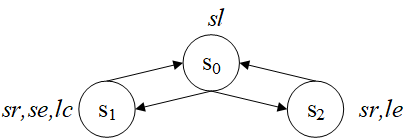
\includegraphics[width=5cm]{BVM.png}\\
%   \caption{An initial \MPK-structure $(\Hm,s_0)$}\label{BBVM}
% \end{figure}

% We verify this result by the following two steps:
% \begin{enumerate}[(i)]
%   \item It is evident that $\varphi \models \psi$ and $\Var(\varphi) \subseteq V$. Besides, $(\Hm, s_0) \models \varphi \wedge \psi$, hence $(\Hm, s_0) \models \varphi \rto \psi$, which means $\varphi$ is a SC of $\psi$ on $V$ under $(\Hm, s_0)$,
%   \item We will show that for any SC $\varphi'$ of $\psi$ on $V$ under $(\Hm, s_0)$,  we have $(\Hm, s_0) \models \varphi' \rto \varphi$. Following Figure~\ref{carVB}, we can see that $(\Hm', s_0) \lrto_{\Ha - V} (\Hm, s_0)$. By Theorem~\ref{CF} we can easily obtain the characterizing formula of $(\Hm, s_0)$ on $V$, \ie ${\cal F}_V(\Hm, s_0)\equiv {\cal F}_V(\Hm', s_0) = sl \wedge \neg sr \wedge \ALL\GLOBAL ((sl \wedge \neg sr) \rto \ALL \NEXT (\neg sl \wedge sr)) \wedge \ALL \GLOBAL((\neg sl \wedge sr) \rto \ALL\NEXT (sl \wedge \neg sr))$, due to $ch(\Hm', \Ha - V) =0$.

%       If ${\cal F}_V(\Hm', s_0) \not \models \varphi'$ or $\varphi' \models \neg sl$ then we have ${\cal F}_V(\Hm', s_0) \models \varphi' \rto \varphi$ i.e. $(\Hm, s_0) \models \varphi' \rto \varphi$. Therefore, we suppose ${\cal F}_V(\Hm', s_0) \models \varphi'$. In this case we can construct $\varphi'$ as follows: (1) $sl$ is a sub-formula of $\varphi'$ due to ${\cal F}_V(\Hm', s_0) \models \varphi'$; (2) $sl \rto \ALL\NEXT sr$ is also a sub-formula by (1),  $(\Hm, s_0) \models \varphi' \rto \psi$ and $\Var(\varphi') \subseteq V$. This means that each SC $\varphi'$ should be the following form with $\beta$ is a \CTL\ formula of $V$:
%       \[
%       (sl \wedge (sl \rto \ALL\NEXT sr)) \wedge \beta.
%       %;\ \  (sl \wedge (sl \rto \ALL\NEXT sr)) \vee \beta.
%       \]
%     In this case, we have $(\Hm, s_0) \models \varphi' \rto \varphi$ for all SC $\varphi'$ of $\psi$ on $V$ under $(\Hm, s_0)$ since for any $\alpha$ with $\Var(\alpha) \subseteq V$ $(\Hm, s_0) \models \alpha$ iff $(\Hm', s_0) \models \alpha$ by Theorem~\ref{thm:V-bisimulation:EQ}.
% \end{enumerate}

% \begin{figure}[ht]
%   \centering
%   % Requires \usepackage{graphicx}
%   \includegraphics[width=3cm]{carVB.png}\\
%   \caption{An initial \MPK-structure $(\Hm',s_0)$}\label{carVB}
% \end{figure}





\begin{proposition}[Dual]\label{dual}
%(\textbf{dual})
 Let $V,q,\varphi$ and $\psi$ are defined as in Definition~\ref{def:NC:SC}.
 Then, $\psi$ is a SNC (WSC) of $q$ on $V$ under $\varphi$ iff $\neg \psi$ is a WSC (SNC)
    of $\neg q$ on $V$ under $\varphi$.
% \begin{enumerate}[(i)]
%   \item $\psi$ is a SNC of $q$ on $V$ under $\varphi$ iff $\neg \psi$ is a WSC
%    of $\neg q$ on $V$ under $\varphi$.
%   \item $\psi$ is a WSC of $q$ on $V$ under $\varphi$ iff $\neg \psi$ is a  SNC
%    of $\neg q$ on $V$ under $\varphi$.
% \end{enumerate}
\end{proposition}
% \begin{proof}
%      (i) Suppose $\psi$ is the SNC of $q$. Then $\varphi \models q \rto \psi$. Thus $\varphi \models \neg \psi \rto \neg q$. So $\neg \psi$ is a
% SC of $\neg q$. Suppose $\psi'$ is any other SC of $\neg q$: $\varphi \models \psi' \rto \neg q$. Then $\varphi \models q \rto \neg \psi'$, this means $\neg \psi'$ is a NC of $q$ on $V$ under $\varphi$.
% Thus $\varphi \models \psi \rto \neg \psi'$ by the assumption. So $\varphi \models \psi' \rto \neg \psi$. This proves that $\neg \psi$ is the WSC of $\neg q$.
% The proof of the other part of the proposition is similar.

% (ii) The WSC case can be proved similarly with SNC case.
%     \end{proof}
%Under this dual property, we can bother ourselves with only one of them e.g., SNC,  and WSC can be obtained easily. %\begin{proof}
%
%\end{proof}



In order to generalise Definition~\ref{def:NC:SC} to arbitrary formulas, one can replace $q$ (in the definition)  by any formula $\alpha$, and redefine  $V$ as a subset of $\Var(\alpha) \cup \Var(\phi)$.
%  For the case of formula, we have that the SCN (WSC) of any formula can be defined as follows:
%\begin{definition}\label{formulaNS}
   % Let $\Gamma$ be a formula or an initial \MPK-structure, $\alpha$ be a formula and $P\subseteq (\Var(\Gamma) \cup \Var(\alpha))$. A formula $\varphi$ of $P$ is  said to be a NC (SC) of $\alpha$ on $P$ under $\Gamma$ iff $\Gamma \models \alpha \rto \varphi$. It is said to be a SNC (WSC) if it is a NC (SC), and for any other NC (SC) $\varphi'$, we have that $\Gamma \models \varphi \rto \varphi'$ ($\Gamma \models \varphi' \rto \varphi$).
   % \end{definition}
    It turns out that the previous notions of SNC and WSC for an atomic variable can be lifted to any formula, or, conversely, the SNC and WSC of any formula can be reduced to that of an atomic variable, as the following result shows.
\begin{proposition}\label{formulaNS_to_p}
     Let $\Gamma$ and $\alpha$ be two formulas, $V \subseteq \Var(\alpha) \cup \Var(\Gamma)$  and $q$ be a new proposition not in $\Gamma$ and $\alpha$.
 Then, a formula $\varphi$ of $V$ is the SNC (WSC) of $\alpha$ on $V$ under  $\Gamma$ iff it is the SNC (WSC) of $q$ on $V$ under $\Gamma' = \Gamma \cup \{q \lrto \alpha\}$.
 \end{proposition}
%  \begin{proof}
%     We prove this for SNC. The case for WSC is similar.
%     Let $\emph{SNC}(\varphi,\alpha,V,\Gamma)$ denote that $\varphi$ is the SNC of $\alpha$ on $V$ under $\Gamma$, and  $\emph{NC}(\varphi,\alpha,V,\Gamma)$ denote that $\varphi$ is the NC of $\alpha$ on $V$ under $\Gamma$.

%     ($\Rto$) We will show that if $\emph{SNC}(\varphi,\alpha,V,\Gamma)$ holds, then $\emph{SNC}(\varphi,q,V,\Gamma')$ will be true. According to $\emph{SNC}(\varphi,\alpha,V,\Gamma)$ and $\alpha\equiv q$, we have $\Gamma' \models q\rto \varphi$, which means $\varphi$ is a NC of $q$ on $V$ under $\Gamma'$. Suppose $\varphi'$ is any NC of $q$ on $V$ under $\Gamma'$, then $\CTLforget(\Gamma',q)\models \alpha \rto \varphi'$ due to $\alpha\equiv q$, $\emph{IR}(\alpha \rto \varphi', \{q\})$ and $(\PP)$, i.e., $\Gamma \models \alpha \rto \varphi'$ by Lemma \ref{lem:KF:eq}, this means $\emph{NC}(\varphi',\alpha,V,\Gamma)$. Therefore, $\Gamma \models \varphi \rto \varphi'$ by the definition of SNC and $\Gamma' \models \varphi \rto \varphi'$. Hence, $\emph{SNC}(\varphi,q,V,\Gamma')$ holds.

%     ($\Lto$) We will show that if $\emph{SNC}(\varphi,q,V,\Gamma')$ holds, then $\emph{SNC}(\varphi,\alpha,V,\Gamma)$ will be true. According to $\emph{SNC}(\varphi,q,V,\Gamma')$, it's not difficult to know that $\CTLforget(\Gamma', \{q\})\models \alpha \rto \varphi$ due to $\alpha\equiv q$, $\emph{IR}(\alpha \rto \varphi, \{q\})$ and $(\PP)$, i.e., $\Gamma \models \alpha \rto \varphi$ by Lemma \ref{lem:KF:eq}, this means $\emph{NC}(\varphi,\alpha,V,\Gamma)$. Suppose $\varphi'$ is any NC of $\alpha$ on $V$ under $\Gamma$. Then $\Gamma' \models q \rto \varphi'$ since $\alpha\equiv q$ and $\Gamma'=\Gamma \cup \{q\lrto \alpha\}$, which means $\emph{NC}(\varphi',q,V,\Gamma')$. According to $\emph{SNC}(\varphi,q,V,\Gamma')$, $\emph{IR}(\varphi \rto \varphi', \{q\})$ and $(\PP)$, we have
%     $\CTLforget(\Gamma', \{q\})\models \varphi \rto \varphi'$, and $\Gamma \models \varphi \rto \varphi'$ by Lemma \ref{lem:KF:eq}. Hence, $\emph{SNC}(\varphi,\alpha,V, \Gamma)$ holds.
%     \end{proof}

To give an intuition for WSC, we give the following example. The intuition for SNC is dual.

\begin{example}[cont'd from Example~\ref{ex:2}]\label{examp:WSC}
Recall ${\cal K}_2$ in Figure~\ref{v1uv2}. Let $\psi = \EXIST \NEXT(s \wedge (\EXIST \NEXT se \vee \EXIST \NEXT \neg d))$, $\varphi = \EXIST \NEXT(s \wedge \EXIST \NEXT \neg d)$, $\Ha =\{d, s, se\}$ and $V = \{s, d\}$, then we can check  that the WSC of $\psi$ on $V$ under ${\cal K}_2$ is $\varphi$.

We verify this result by the following two steps:
\begin{enumerate}[(i)]
  \item Observe that $\varphi \models \psi$ and $\Var(\varphi) \subseteq V$. Besides, $(\Hm, s_0) \models \varphi \wedge \psi$, hence ${\cal K}_2 \models \varphi \rto \psi$, which means $\varphi$ is a SC of $\psi$ on $V$ under ${\cal K}_2$,
  \item We will show that for any SC $\varphi'$ of $\psi$ on $V$ under ${\cal K}_2$,  we have ${\cal K}_2 \models \varphi' \rto \varphi$. It is easy to see that if ${\cal K}_2 \not \models \varphi'$, then ${\cal K}_2\models \varphi' \rto \varphi$, trivially. Now let's assume ${\cal K}_2 \models \varphi'$. In this case, we have $\varphi' \models \psi$ since $\varphi'$ is a SC of $\psi$ on $V$ under ${\cal K}_2$. Therefore, there is $\varphi' \models \EXIST \NEXT(s \wedge \phi)$, in which $\phi$ is a formula such that $\phi\models \EXIST \NEXT se \vee \EXIST \NEXT \neg d$. And then $\phi \models \EXIST \NEXT \neg d$ since $\IR(\varphi', \overline V)$. Hence, $\varphi' \models \varphi$ and we get  ${\cal K}_2 \models \varphi' \rto \varphi$, as desired.
\end{enumerate}
\end{example}

The following result establishes the bridge between forgetting and the notion of SNC (WSC) which are central to our contribution.

%; basically  SNC (WSC)  and the forgetting in which the former is obtained through the latter.
%In particular, it shows  how SNC  (WSC) of a property $q$ is obtained through the operation of forgetting.

\begin{theorem}\label{thm:SNC:WSC:forget}
 Let $\varphi$ be a formula, $V\subseteq\Var(\varphi)$ and $q\in\Var(\varphi)- V$.
 \begin{enumerate}[(i)]
   \item $\CTLforget (\varphi \land q$, $(\Var(\varphi) \cup \{q\}) - V)$
   is a SNC of $q$ on $V$ under $\varphi$.
   \item  $\neg\CTLforget (\varphi \land \neg q$, $(\Var(\varphi) \cup \{q\}) - V)$
   is a WSC of $q$ on $V$ under $\varphi$.
 \end{enumerate}
 \end{theorem}
%  \begin{proof}
%  We will prove the SNC part, while it is not difficult to prove the WSC part according to Proposition \ref{dual}.
%  Let ${\cal F}=\CTLforget(\varphi \wedge q, (\Var(\varphi) \cup \{q\})- V)$.

%   The ``NC" part: It's easy to see that $\varphi \wedge q \models {\cal F}$ by {\bfseries (W)}. Hence, $\varphi\models q \rto {\cal F}$, this means
%   ${\cal F}$ is a NC of $q$ on $V$ under $\varphi$.

%   %  $\Gamma \models q \rto F$\\
% %    $\Gamma \wedge q \models F$    \quad \quad \quad $(W)$\\
% %    $\Rto$ $\Gamma\models q \rto F$   \quad \quad \quad $(\rightarrow +)$\\
% %    \\
%     %  The ``SNC" part: We will show that for all NC $\psi'$ of $q$ on $V$ under $\varphi$ there is $\varphi \models {\cal F} \rto \psi'$.
%     %  Suppose that there is a NC $\psi$ of $q$ on $V$ under $\varphi$ with $\psi$ is not logical equivalence with ${\cal F}$ under $\varphi$ such that $\varphi \models \psi \rto {\cal F}$.
%     %  We know that $\varphi \wedge q \models \psi$ iff ${\cal F} \models \psi$ by {\bfseries (PP)} due to $\emph{IR}(\psi, (\Var(\varphi) \cup \{q\})- V)$. Hence, $\varphi \wedge {\cal F} \models \psi$ by $\varphi \wedge q \models \psi$ (by the assumption).
%     %  Moreover, we have that $\varphi \wedge \psi \models {\cal F}$ by the assumption. Therefore, there is $\varphi \models \psi \lrto {\cal F}$, which means $\psi$ is logic equivalence with ${\cal F}$ under $\varphi$.
%     %  This is contradict with the suppose. Then ${\cal F}$ is the SNC of $q$ on $V$ under $\varphi$.

%      The ``SNC" part: We will show that for all NC $\psi'$ of $q$ on $V$ under $\varphi$ (i.e $\varphi\models q \rto \psi'$) there is $\varphi \models {\cal F} \rto \psi'$.
%     We know that if $\varphi \wedge q \models \psi'$ then ${\cal F} \models \psi'$ by {\bfseries (PP)} due to $\emph{IR}(\psi', (\Var(\varphi) \cup \{q\})- V)$. Therefore, we have $\varphi \wedge {\cal F} \models \psi'$ since $\psi'$ is a NC of $q$ on $V$ under $\varphi$ and then $\varphi \models {\cal F} \rto \psi'$, i.e.  ${\cal F}$ is the SNC of $q$ on $V$ under $\varphi$.
%  \end{proof}

% \textcolor{red}{Intuitively, the result of forgetting a set $V$ of propositions from a formula $\varphi$ is the strongest one among formulas which are $V$-irrelevant and models of $\varphi$, due to (\W) and (\PP). }

Following Theorem~\ref{thm:SNC:WSC:forget}, assume that $\beta = \CTLforget(\varphi \wedge q, (\Var(\varphi) \cup \{q\})- V)$.  Then, $\varphi \wedge q \models \beta$  by (\W). Moreover,  $\varphi \wedge q \models \beta$,  and then $\beta$ is a NC of $q$ on $V$ under $\varphi$.
%In  Theorem~\ref{thm:SNC:WSC:forget}, assume that ${\cal F} = \CTLforget(\varphi \wedge q, (\Var(\varphi) \cup \{q\})- V)$, we can see that $\varphi \wedge q \models {\cal F}$ by (\W)  and then ${\cal F}$ is a NC of $q$ on $V$ under $\varphi$.
In addition, for any $\psi$ with $\IR(\psi, (\Var(\varphi) \cup \{q\})- V)$ and $\varphi \wedge q \models \psi$, %(and hence $\varphi \models \psi$ due to $\IR(\psi, \{q\})$),
we have $\beta \models \psi$ by (\PP). Therefore, $\beta$ is the SNC of $q$ on $V$ under $\varphi$. This shows the intuition of how the SNC can be obtained from the forgetting.

Since any initial $\MPK$-structure can be characterized by a \CTL\ formula, by  Theorem~\ref{thm:SNC:WSC:forget} one can obtain the SNC (and its dual WSC) of a target property (a formula) under an initial $\MPK$-structure just by forgetting. This is shown in the following result.
\begin{theorem}\label{thm:inK:SNC}
Let ${\cal K}= (\Hm, s)$ be an initial \MPK-structure with $\Hm=(S,R,L,s_0)$ on the set $\Ha$ of atoms, $V \subseteq \Ha$ and $q\in V' = \Ha - V$. Then,
 \begin{enumerate}[(i)]
   \item the SNC of $q$ on $V$ under ${\cal K}$ is $\CTLforget({\cal F}_{\Ha}({\cal K}) \wedge q, V')$.
   \item the WSC of $q$ on $V$ under ${\cal K}$ is $\neg \CTLforget({\cal F}_{\Ha}({\cal K}) \wedge \neg q, V')$.
 \end{enumerate}
\end{theorem}
%\label{thm:inK:SNC}\begin{proof}
%(i)
%As we know that any initial \MPK-structure ${\cal K}$ can be described as a characterizing formula ${\cal F}_{\Ha}({\cal K})$, then the SNC of $q$ on $V$ under ${\cal F}_{\Ha}({\cal K})$ is $\CTLforget({\cal F}_{\Ha}({\cal K}) \wedge q, \Ha - V)$. We will prove that $\CTLforget({\cal F}_{V \cup \{q\}}({\cal K}_{|V \cup \{q\}}) \wedge q, q)  \equiv  \CTLforget({\cal F}_{\Ha}({\cal K}) \wedge q, \Ha - V)$.
%
%($\Rto$) $\forall {\cal K}_1 \in \Mod(\CTLforget({\cal F}_{V \cup \{q\}}({\cal K}_{|V \cup \{q\}}) \wedge q, q))$\\
%$\Rto$ there is an initial \MPK-structure ${\cal K}'$ such that ${\cal K}' \models {\cal F}_{V \cup \{q\}}({\cal K}_{|V \cup \{q\}}) \wedge q$ and ${\cal K}_1 \lrto_{\{q\}} {\cal K}'$\\
%$\Rto$ ${\cal K}' \lrto_{\Ha-(V\cup \{q\})} {\cal K}_{|V \cup \{q\}}$  \hfill (Theorem~\ref{CF})\\
%$\Rto$ ${\cal K}_1 \lrto_{\Ha-V} {\cal K}_{|V \cup \{q\}}$   \hfill (Proposition~\ref{div})\\
%$\Rto$ ${\cal K}_{|V \cup \{q\}} \lrto_{\Ha-(V \cup \{q\})} {\cal K}$   \hfill  (Proposition~\ref{pro:VQ})\\
%$\Rto$ ${\cal K}' \lrto_{\Ha-(V\cup \{q\})} {\cal K}$  \hfill (Proposition~\ref{div})\\
%$\Rto$ ${\cal K} \models {\cal F}_{\Ha}({\cal K}) \wedge q$\\
%$\Rto$ ${\cal K}_1 \lrto_{\Ha -V} {\cal K}$\\
%$\Rto$ ${\cal K}_1 \models \CTLforget({\cal F}_{\Ha}({\cal K}) \wedge q, \Ha - V)$
%
%$(\Lto)$ $\forall {\cal K}_1 \in \Mod(\CTLforget({\cal F}_{\Ha}({\cal K}) \wedge q, \Ha - V))$ \\
%$\Rto$ there an initial \MPK-structure ${\cal K}_2$ s.t.\ ${\cal K}_2 \models {\cal F}_{\Ha}({\cal K}) \wedge q$ and ${\cal K}_1 \lrto_{\Ha - V} {\cal K}_2$\\
%$\Rto$ ${\cal K}_2 \lrto_{{\Empty}} {\cal K}$   \hfill (Theorem~\ref{CF})\\
%$\Rto$ ${\cal K}_2 \lrto_{\Ha-(V\cup \{q\})} {\cal K}_{|V \cup \{q\}}$ due to ${\cal K}_{|V \cup \{q\}} \lrto_{\Ha-(V \cup \{q\})} {\cal K}$   \hfill  (Proposition~\ref{pro:VQ})\\
%$\Rto$ ${\cal K}_2 \models {\cal F}_{V \cup \{q\}}({\cal K}_{|V \cup \{q\}}) \wedge q$  \\
%$\Rto$ ${\cal K}_1 \models \CTLforget({\cal F}_{V \cup \{q\}}({\cal K}_{|V \cup \{q\}}) \wedge q, q)$.
%
%(ii) This is proved by the dual property.
%\end{proof}

%\begin{example}
%For the Example~\ref{exmp:1}, the WSC of $\varphi$ on $V$ under ${\cal K} =(\Hm, s_0)$ is $\neg \CTLforget({\cal F}_{\Ha}({\cal K}) \wedge (q \lrto \varphi) \wedge \neg q, \Ha - V)$.
%\end{example}

\section{An Algorithm for Forgetting in \CTL\ }
\label{section_algorithm}
The technical developments we have presented in previous sections naturally induce a procedure to compute forgetting in CTL. We think that it is useful to outline such a procedure explicitly in the form of an algorithm.  It is a model-based approach (presented in Algorithm~\ref{alg:compute:forgetting:by:VB}); that is,  it will compute the forgetting applied to a formula, simply  by considering all the possible models of that formula.  Its correctness is guaranteed by Lemma~\ref{lem:models:formula} and Theorem~\ref{CF}.
%By the definition of forgetting in \CTL, the set of models of the result of forgetting is also a finite set of initial \MPK-structures.
%To compute the forgetting in \CTL, we propose a model-based method in this part.
%Literally speaking, the model-based method means that we can obtain the result of forgetting in \CTL\ by obtain all the possible finite models of this result.
%% How can we obtain all the \MPK-models is what we will solved in this part.
%%The resolution-based method obtain the result of forgetting by obtaining all the possible resolutions which can be implied by the original formula.

%As we have said that the set of models of any formula $\varphi$ is finite, hence if we can obtain all the models of $\varphi$ then we can express this formula by the disjunction of those characteristic formulas of those models.
%By the definition of forgetting in \CTL, the set of models of the result of forgetting is also a finite set of initial \MPK-structures.
%Then the model-based method is generated for forgetting in \CTL.
%
%Though the set of models of the result of forgetting is finite, while how many models is there?
%%That's right we should given the bound of the number of the models.
%As it is said in Theorem~\ref{thm:VBChFEQ} that if two initial \MPK-structures are $V$-bisimulation, then their characteristic formulas is equal.

%Then let $\varphi$ be a CTL formula, the $|\Var(\varphi)|=m$ is a positive integer, we have the following theorem:
%\begin{theorem}
%Let $\varphi$ be a CTL formula, $V=\Var(\varphi)$, $|V|=m$, and ${\cal K}=(\Hm, s_0)$ with $\Hm=(S, R,L,s_0)$ be a initial \MPK-structure. If $(\Hm, s_0) \models \varphi$, then there is an initial \MPK-structure ${\cal K}'=(\Hm', s_0')$ with $\Hm'=(S', R',L',s_0')$ that satisfy:
%\begin{enumerate}[(i)]
%  \item $|S'|$ is at most $2^m$,
%  \item $|R'|$ is at most $2^m * 2^m$,
%  \item $|L'|$ is at most $2^m * 2^m$,
%  \item ${\cal K} \lrto_{\Ha - V} {\cal K}'$ and $(\Hm', s_0') \models \varphi$.
%\end{enumerate}
%\end{theorem}
%\begin{proof}
%If $|S| \leq 2^m$, this result clearly holds. If $|S| > 2^m$, let ${\cal K}' = {\cal K}_{|V}$, then it is apparent that ${\cal K} \lrto_{\Ha - V} {\cal K}'$ by Proposition~\ref{pro:VQ} and $(\Hm', s_0') \models \varphi$. In the worst case, the number of states in $S'$ is $2^m$ by the definition of ${\cal K}_{|V}$. Then the theorem is proved.
%\end{proof}

%By this theorem, we can see that any initial \MPK-structures ${\cal K}$ that satisfy $\varphi$ can be transformed to an initial \MPK-structure ${\cal K}'$ such that ${\cal K} \lrto_{\Ha - V} {\cal K}'$ and ${\cal K} \models \varphi$ iff ${\cal K}' \models \varphi$ due to $\IR(\varphi, \Ha- V)$, in which $V= \Var(\varphi)$. Therefore, the size of the model of $\varphi$ is at most $2^m$ by Theorem~\ref{thm:VBChFEQ}(we only consider the number of states of this model).

% we give a trivial algorithm computing \CTL\ forgetting result, . % to compute the forgetting in CTL.


\begin{algorithm}[tb]
	\caption{\small A model-based \CTL\ forgetting procedure}
	\label{alg:compute:forgetting:by:VB}
	\KwIn{A \CTL formula $\varphi$ and a set $V$ of atoms}
	\KwOut{$\CTLforget(\varphi, V)$}% ????
	$\psi \lto \bot$\;
	\ForEach{initial \MPK-structure $\cal K$ (over $\cal A$ and $\cal S$)}{
		\lIf{${\cal K}\not\models\varphi$}{{\bf continue}} %\;
		\ForEach{initial \MPK-structure ${\cal K}'$ with ${\cal K}\lrto_{ V}{\cal K}'$}{
			$\psi \lto \psi \lor {\cal F}_{\overline V}({\cal K}')$\;
		}
	}
	\Return $\psi$\;
\end{algorithm}
%%
%%\begin{algorithm}[tb]
%%\caption{A Model-based Forgetting Procedure}
%%\label{alg:compute:forgetting:by:VB}
%%\KwIn{A CTL formula $\varphi$ and a set $V$ of atoms}
%%\KwOut{$\CTLforget(\varphi, V)$}% ????
%%$T={\Empty}$ // the set of models of $\varphi$ \;
%%$T' = {\Empty}$ // the set of possible initial \MPK-structures \;
%%%$m=|\Var(\varphi)|$\;
%%$n=|\Ha|$\;
%%
%%\For {$i=1, ..., 2^n$}{
%%       % Enumerating all possible initial \MPK-structures $(\Hm, s_0)$ with $\Hm=(S, R, L,s_0)$ and $|S|=i$\;
%%        \For {$s_j\in \{s_1, \dots, s_i\}$}{
%%            Let $s_j$ be an initial state, construct $\Hm=(S, R, L,s_j)$ by the definition of model structure with $S=\{s_1, \dots, s_i\}$\;
%%            \For {${\cal K}\in T'$} {
%%             \If {$(\Hm, s_j) \nleftrightarrow_{\overline {\Var(\varphi)}} \cal K$}{
%%                 Let $T' \leftarrow T' \cup \{(\Hm, s_j)\}$\;
%%             }
%%             }
%%        }
%%        \For {$(\Hm, s_0) \in T'$ }{
%%            \If {$(\Hm,s_0) \models \varphi$}{
%%                $T \leftarrow T \cup \{(\Hm,s_0)\}$\;
%%            }
%%        }
%%       % For all initial \MPK-structures $(\Hm, s_0)$ \If {$(\Hm,s_0) \models \varphi$}{
%%%            $T= T \cup \{(\Hm,s_0)\}$\;
%%%        }
%%}
%%%\For {${\cal K} =(\Hm, s_0) \in T$} {
%%%    Let $T' = T' \cup \{{\cal K}_{|V} \}$\;
%%%}
%%%
%%%\For {i=1, ..., $2^{m-n}$}{
%%%        Enumerating all possible initial \MPK-structures $(\Hm', s_0')$ with $\Hm'=(S', R', L',s_0')$ and $|S'|=i$\;
%%%        For all initial \MPK-structures $(\Hm', s_0')$ \If {$\exists (\Hm,s_0)\in T$ s.t. $(\Hm,s_0) \lrto_V (\Hm', s_0')$}{
%%%            $T'= T' \cup \{(\Hm',s_0')\}$\;
%%%        }
%%%}
%%\Return $\bigvee_{(\Hm', s_0')\in T} {\cal F}_{\overline V}(\Hm', s_0')$.
%%\end{algorithm}

The example we give below echoes the initial example which was given in the introduction, and finalizes the running example with a simple intuition of forgetting.
\begin{example}\label{ex:6}
%Consider the model given in Figure~\ref{BBVM}.
Recall the \MPK-structure ${\cal K}_1$  given in Figure~\ref{v1uv2}, and assume that we are given a property $\alpha = \EXIST\FUTURE(se \wedge sp)$. It is easy to see that ${\cal K}_1$ in Figure~\ref{v1uv2} satisfy $\alpha$. If $sp$ is intended to be removed, i.e., forgetting  $sp$ from $\alpha$,  then  $\CTLforget(\alpha,\{ sp\}) \equiv \EXIST\FUTURE se$. Hence, the company can use the new specification $\EXIST\FUTURE se$ to guide the new production process (which guarantees that the sedan car is eventually produced).
\end{example}
%\begin{example}
%Let $\varphi=\ALL\GLOBAL \ALL\FUTURE (p \wedge r)$, $\Ha=\{p,r\}$ and $V=\{r\}$. For convenience, we use the label of a state to express the state and then remove the label function in a model structure.
%Let $\Hm_1=(\{\{p,r\}\}, \{(\{p,r\}, \{p,r\})\}, \{p,r\})$ and $\Hm_2=(\{\emptyset,\{p,r\}\}, \{(\emptyset, \{p,r\})$, $(\{p,r\}$, $\{p,r\})\}, \emptyset)$.
%\Hm_3=(\{\emptyset,\{p\}$, $\{p,r\}\}$, $\{(\emptyset$, $\{p\})$, $(\{p\}$, $\{p, r\})$, $(\{p, r\}$, $\emptyset)\}$, $\emptyset)$,
%The set of models of $\varphi$ is $\Mod(\varphi)=\{(\Hm_1, \{p\})$, $(\Hm_2$, $\emptyset), \dots\}$.

%Let $\Hm_1'=(\{\{p\}\}, \{(\{p\}, \{p\})\}, \{p\})$ and $\Hm_2'=(\{\emptyset,\{p\}\}, \{(\emptyset, \{p\})$, $(\{p\}$, $\{p\})\}, \emptyset)$
%  Then we can obtain all the possible initial \MPK-structure that is a model of $\CTLforget(\varphi, V)$, i.e., $\Mod(\CTLforget(\varphi, V)) =\{{\cal K}_1=(\Hm_1', \{p\}), {\cal K}_2=(\Hm_2', \emptyset), \dots\}$.

%Let $V'=\{p\}$, ${\cal K}_1=(\Hm_1, \{p,r\})$ and ${\cal K}_2=(\Hm_2, \emptyset)$, then
 %${\cal F}_{V'}({\cal K}_1)= p \wedge \ALL\GLOBAL (p\rto  \ALL \NEXT p)$,
 %and
% ${\cal F}_{V'}({\cal K}_2)=\neg p\wedge \ALL\GLOBAL (p\rto  \ALL \NEXT \neg p) \wedge \ALL\GLOBAL (\neg p\rto  \ALL \NEXT p)$. Similarly, we can obtain the characteristic formula of other models and then the $\CTLforget(\varphi, V)$.% is the disjunction of all the characteristic formulae of those models.
%\end{example}

As we will show below, computing the forgetting by going through all the models is not very efficient, as one might expect. However, settling it is important from a theoretical point of view i.e., to see how costly is the naive approach.

\begin{proposition}\label{pro:time:alg1}
Let $\varphi$ be a \CTL\ formula and $V\subseteq \Ha$ with $|{\cal S}|=m$, $|\Ha|=n$ and $|V|=x$. Then the space complexity is $O((n-x)m^{2(m+2)}2^{nm}  \log m)$ and the time complexity of Algorithm~\ref{alg:compute:forgetting:by:VB} is at least the same as the space.%and the space complexity is $O(2^{2m})$, where $|\Ha| = m$.
\end{proposition}
%\begin{proof}
%Suppose that each state or atom occupies $\log m$ (supposing $n\leq m$), then a state pair $(s, s')$ occupies $2* \log m$ bits.
%For any $B\subseteq {\cal S}$ with $B \not = \emptyset$ and $s_0\in B$, we can construct an initial \MPK-structure $(\Hm, s_0)$ with $\Hm=(B, R, L, s_0)$, in which there is at most $\frac{|B|^2}{2}$ state pairs in $R$ and $|B|*n$ pairs $(s, A)$ ($A \subseteq \Ha$) in $L$. Hence, the $(\Hm, s_0)$ requires at most $(|B|+|B|^2 + |B|*n)*\log m$ bits.
%Besides, for the set $B$ of states we have $|B|$ choices for the initial state, $|B|^{|B|}$ choices for the $R$ and $(2^n)^{|B|}$ choices for the $L$. In the worst case, i.e., when $|B|=m$, we have $m*(m^m * 2^{nm} * m)$ number of initial \MPK-structures.
%Therefore, there is at most $m^{m+2}*2^{nm}$ number of initial \MPK-structures, hence it will cost at most  $(m^{m+2}*2^{nm}*(m+m^2+nm))*\log m$ bits.

%Let $k=n-x$, for any initial \MPK-structure ${\cal K}=(\Hm, s_0)$ with $i\geq 1$ nodes and $\Hm=(B, R, L, s_0)$, in the worst case, i.e., when $ch(\Hm,V)=i$, we will require  a space of $N(i)=P_i(s_0) + i * (P_i(s) + i * P_i(s'))$  to store the characterizing formula of ${\cal K}$ on $\overline{V}$  where $s', s\in B$ and $P_i(y)$ is the space required to store ${\cal F}_{\overline{V}}(\Tr_i(y))$ with $y\in B$.
%(We suppose the formulas in $\EXIST \NEXT$ and $\ALL \NEXT$ parts share the same memory.)
%In the following, we compute inductively the space required to store the ${\cal F}_{\overline{V}}(\Tr_n(y))$ with $0\leq n \leq i$
%\begin{align*}
%    & (1)\ n = 0, && P_0(y) = k\\ % \text{i.e. the number of atoms in \overline{V}}\\
%    & (2)\ n =1, && P_1(y) = k + i *k = k + i* P_0(y)\\
%    & (3)\ n =2, && P_2(y) = k + i*(k + i*k) \\
%    &   && \qquad \ = k + i*P_1(y)\\
%    & \dots && \dots\\
%    & (i+1)\ n = i, && P_i(y) =k+ i *P_{i-1}(y).
%\end{align*}
%Therefore, we have
%\begin{align*}
% P_i(y) &= k + i*k+ i^2*k\dots + i^i * k = \frac{i^i -1}{i-1} k, \text{ and }\\
% N(i)&= P_i(s_0) + i * (P_i(s) + i * P_i(s'))\\
% = & (i^2 +i +1) P_i(y)\\
% =& (i^2+i +1) \frac{i^i -1}{i-1} k.
%\end{align*}
%In the worst case, i.e., there is $m^{m+2}*2^{nm}$ initial \MPK-structures with $m$ nodes, we will need $(m^{m+2}*2^{nm}*N(m))*\log m$ bits to store the result of forgetting.

% It is obvious that computing the $V$-characterization number of any initial \MPK-structure $\cal K$ does not more than $O(i^2P)$ with $P$ expressing a polynomial function.
%Therefore, the space complexity is $O((n-x)m^{2(m+2)}2^{nm} * \log m)$ and the time complexity is at least the same as the space.
%\end{proof}

As expected, Algorithm~\ref{alg:compute:forgetting:by:VB} has a high cost; namely, \textsc{ExpSpace} complexity in the size of the state space and $\Ha$, which does not look encouraging. However, we believe that settling this result is important both from a theoretical and a practical point of view. Theoretically, it gives us a picture about the worst case, and urges us to come up with more efficient syntactical approaches which is a part of our future agenda. Moreover, we believe that model-based investigation and some of the structural observations we have made provide us with  informative valuable insights, which in turn could be useful in designing future algorithms which can exploit these observations, and potentially could lead to even efficient approximations with provably good bounds. Such future developments might prove important in developing practical algorithms as well.







\section{Concluding Remarks}
\label{conclusion}
\paragraph{Summary}
In this paper, we have presented the notion of forgetting for \CTL\
%generalized the notion of bisimulation from initial structures of Computation Tree Logic (\CTL) to initial structures with initial states over a given signature $V$, named $V$-{\em bisimulation}.
which enables computing weakest sufficient and strongest necessary conditions of specifications. In doing so, we introduced and employed the notion of $V$-bisimulation which can be considered as  a simple variable based generalisation of classical bisimulation. Furthermore, we have studied formal properties of forgetting, among them, homogeneity, modularity and commutativity. In particular, we have shown that our notion of forgetting satisfies the existing postulates of forgetting, which means it faithfully extends the notion of forgetting from classical propositional logic and modal logic \SFive\ to \CTL.
On the complexity theory side, we have investigated the model checking and the entailment problems of forgetting in the fragment $\CTL_{\ALL\FUTURE}$, which turn out to be $\textsc{NP}$-complete and range from co-$\textsc{NP}$ to $\Pi_2^\textsc{P}$-completeness, respectively.
% On the complexity theory side, we investigated the model checking of forgetting, which turned out to be $\textsc{NP}$-complete, and the relevant fragment of $\CTL_{\ALL\FUTURE}$ which ranged from co-$\textsc{NP}$ to $\Pi_2^\textsc{P}$-completeness.
And finally, we proposed a model-based algorithm which computes the forgetting of a given formula and a set of variables, and outlined its complexity.




\paragraph{Future work}
Note that, when a transition system $\cal M$ does not satisfy a specification $\phi$, one can evaluate the weakest sufficient condition  $\psi$ over a signature $V$ under which ${\cal M}$ satisfies $\phi$, viz., ${\cal M}\models\psi\rto \phi$ and $\psi$ mentions only atoms from $V$. It is worthwhile to explore how the condition $\psi$ can guide the design of a new transition system ${\cal M}'$ satisfying $\phi$.



Moreover, a further study regarding the computational complexity for other general fragments is required and part of the future research agenda. As mentioned in Section~\ref{section_algorithm}, these high complexity results are encouraging for other syntactic approaches e.g., proof-theoretic. Such investigation can be coupled with fine-grained parameterized analysis, as well as a search for approximation algorithms with provably good accuracy bounds.

\section*{Acknowledgements}
We kindly thank all the anonymous reviewers whose comments improved this work to a great extent.
%The first author is funded by the China Scholarship Council (CSC) grant number 201906670007.
Renyan Feng is funded by China Scholarship Council (CSC) grant number 201906670007.
Renyan Feng and Yisong Wang is supported by the National Natural Science Foundation of P.R. China under Grants 61976065, 61370161 and U1836105.
% The work of Renyan Feng and Yisong Wang is partially supported by the National Natural Science Foundation of
% P.R. China under Grants 61976065, 61370161 and U1836105.
Erman Acar's research is funded by MaestroGraph research programme (NWO) with project number 612.001.552.


%
%\bibliographystyle{kr}
%\bibliography{kr20}

 \clearpage
 \appendix
 \section{Supplementary Material: Proof Appendix}
The results in the appendix follows the order in the text. Additional auxiliary lemmas and propositions in the appendix respect that order as well.\\


  \noindent\textbf{Section \ref{forgetting}   Forgetting in \CTL}\\

  \noindent\textbf{Section \ref{forgetting}.1  $V$-bisimulation}\\

 %\textbf{Proposition}~\ref{Vbi:Equ}
 %Let $V\subseteq\cal A$
 %%${\cal M}_i=(S_i,R_i,L_i,s_0^i)~(i=1,2)$ be initial structures
 %and ${\cal K}_i=({\cal M}_i,s_i)~(i=1,2)$ be \MPK-structures.
 %Then $({\cal K}_1,{\cal K}_2)\in\cal B$ if and only if
 %  \begin{enumerate}[(i)]
 %    \item $L_1(s_1)- V = L_2(s_2)- V$,
 %    \item for every $(s_1,s_1')\in R_1$, there is $(s_2,s_2')\in R_2$
 %    such that $({\cal K}_1',{\cal K}_2')\in \Hb$, and
 %    \item for every $(s_2,s_2')\in R_2$, there is $(s_1,s_1')\in R_1$
 %    such that $({\cal K}_1',{\cal K}_2')\in \Hb$,
 %   \end{enumerate}
 % where ${\cal K}_i'=({\cal M}_i,s_i')$ with $i\in\{1,2\}$.\\
 %\begin{proof}
 %$(\Rto)$
 %(a) It is apparent that $L_1(s_1)- V = L_2(s_2)- V$;
 %(b) %We will show that for each $(s_1, s_1') \in R_1$, there is a $(s_2, s_2')\in R_2$ such that $({\cal K}_1', {\cal K}_2') \in \Hb$.
 %$({\cal K}_1, {\cal K}_2) \in \Hb$ iff $({\cal K}_1, {\cal K}_2) \in \Hb_i$ for all $i \geq 0$, then for each $(s_1, s_1') \in R_1$, there is a $(s_2, s_2')\in R_2$  such that  $({\cal K}_1', {\cal K}_2') \in \Hb_{i-1}$ for all $i > 0$ and then $L_1(s_1')- V = L_2(s_2')- V$. Therefore, $({\cal K}_1', {\cal K}_2') \in \Hb$.
 %(c) %We will show that for each $(s_2, s_2') \in R_1$, there is a $(s_1, s_1')\in R_2$ such that $({\cal K}_1', {\cal K}_2') \in \Hb$.
 % This is similar with (b).
 %
 %$(\Lto)$ (a) $L_1(s_1)- V = L_2(s_2)- V$ implies that $(s_1, s_2) \in \Hb_0$;
 %(b) Condition (ii) implies that for every $(s_1,s_1')\in R_1$, there is $(s_2,s_2')\in R_2$
 %    such that $({\cal K}_1',{\cal K}_2')\in \Hb_i$ for all $i \geq 0$;
 %(c) Condition (iii) implies that for every $(s_2,s_2')\in R_2$, there is $(s_1,s_1')\in R_1$
 %    such that $({\cal K}_1',{\cal K}_2')\in \Hb_i$ for all $i \geq 0$\\
 %$\Rto$ $({\cal K}_1, {\cal K}_2) \in \Hb_i$ for all $i \geq 0$\\
 %$\Rto$ $({\cal K}_1,{\cal K}_2)\in\cal B$.
 %\end{proof}



  \noindent\begin{lemma}\label{lem:B:relations}
   Let  $\Hb_0, \Hb_1,\ldots$ be the ones in the definition of section \ref{forgetting}.1.
   Then,  for each $i\ge 0$,
   \begin{enumerate}[(i)]
      \item $\Hb_{i+1}\subseteq \Hb_i$;
      \item there is a (smallest) $k\ge 0$ such that $\Hb_{k+1}=\Hb_k$;
      \item $\Hb_i$ is reflexive, symmetric and transitive.
   \end{enumerate}
 \end{lemma}
 \begin{proof}
   (i)
   Base: it is clear for $i=0$ by the above definition.

   Step: suppose it holds for $i=n$, i.e., $\Hb_{n+1}\subseteq\Hb_n$. \\
   $(s,s')\in\Hb_{n+2}$\\
   $\Rto$ (a) $(s,s')\in  \Hb_0$,
     (b) for every $(s,s_1)\in R$, there is $(s',s_1')\in R'$
      such that $(s_1,s_1')\in \Hb_{n+1}$, and
     (c)  for every $(s',s_1')\in R'$, there is $(s,s_1)\in R$
     such that $(s_1,s_1')\in \Hb_{n+1}$\\
   $\Rto$ (a) $(s,s')\in  \Hb_0$,
   (b) for every $(s,s_1)\in R$, there is $(s',s_1')\in R'$
      such that $(s_1,s_1')\in \Hb_{n}$ by inductive assumption, and
   (c)  for every $(s',s_1')\in R'$, there is $(s,s_1)\in R$
     such that $(s_1,s_1')\in \Hb_{n}$ by inductive assumption\\
   $\Rto$ $(s,s')\in \Hb_{n+1}$.

   (ii) and (iii) are evident from (i) and the definition of $\Hb_i$.
 \end{proof}


 \noindent\textbf{Lemma}~\ref{lem:equive}  The relation $\lrto_V$ is an equivalence relation.
 \begin{proof}
 It is clear from Lemma~\ref{lem:B:relations} (ii) such that there is a $k \geq $ 0 where $\Hb_k = \Hb_{k+1}$ which is  $\lrto_V$, and it is reflexive, symmetric and transitive by (iii).
 \end{proof}


 \noindent\textbf{Proposition}~\ref{div}
 Let $i\in \{1,2\}$, $V_1,V_2\subseteq\cal A$, $s_i'$s be two states,
   $\pi_i'$s be two paths
 and ${\cal K}_i=({\cal M}_i,s_i)~(i=1,2,3)$ be \MPK-structures
  such that
 ${\cal K}_1\lrto_{V_1}{\cal K}_2$ and ${\cal K}_2\lrto_{V_2}{\cal K}_3$.
  Then:
  \begin{enumerate}[(i)]
   \item $s_1'\lrto_{V_i}s_2'~(i=1,2)$ implies $s_1'\lrto_{V_1\cup V_2}s_2'$;
   \item $\pi_1'\lrto_{V_i}\pi_2'~(i=1,2)$ implies $\pi_1'\lrto_{V_1\cup V_2}\pi_2'$;
   \item for each path $\pi_{s_1}$ of $\Hm_1$ there is a path $\pi_{s_2}$  of $\Hm_2$ such that $\pi_{s_1} \lrto_{V_1} \pi_{s_2}$, and vice versa;
   \item ${\cal K}_1\lrto_{V_1\cup V_2}{\cal K}_3$;
   \item If $V_1 \subseteq V_2$ then ${\cal K}_1 \lrto_{V_2} {\cal K}_2$.
  \end{enumerate}
 \begin{proof}
 In order to distinguish the relations $\Hb_0, \Hb_1, \dots$ for different set $V \subseteq \Ha$, by $\Hb_i^V$ we mean the relation $\Hb_1, \Hb_2, \dots$ for $V \subseteq \Ha$.
 Denote as $\Hb_0, \Hb_1, \dots$ when the underlying set $V$ is clear from the context. Moreover, for the ease of notation, we will refer to $\lrto_V$ by $\Hb$ (i.e., without subindex).

 (i) Base: it is clear for $n = 0$.\\
 Step: For $n > 0$, supposing if $({\cal K}_1, {\cal K}_2) \in \Hb_i^{V_1}$ and $({\cal K}_1, {\cal K}_2) \in \Hb_i^{V_2}$ then $({\cal K}_1, {\cal K}_2) \in \Hb_i^{V_1 \cup V_2}$ for all $0 \leq i \leq n$. We will show that if $({\cal K}_1, {\cal K}_2) \in \Hb_{n+1}^{V_1}$ and $({\cal K}_1, {\cal K}_2) \in \Hb_{n+1}^{V_2}$ then $({\cal K}_1, {\cal K}_2) \in \Hb_{n+1}^{V_1 \cup V_2}$.\\
 (a) It is evident that $L_1(s_1) - (V_1 \cup V_2) = L_2(s_2) - (V_1\cup V_2)$.\\
 (b) We will show that for each $(s_1, s_1^1) \in R_1$ there is a $(s_2, s_2^1) \in R_2$ such that $(s_1^1, s_2^1) \in \Hb_n^{V_1 \cup V_2}$. There is $({\cal K}_1^1, {\cal K}_2^1) \in \Hb_{n-1}^{V_1 \cup V_2}$
 due to $({\cal K}_1, {\cal K}_2) \in \Hb_n^{V_1 \cup V_2}$ by inductive assumption. Then we only need to prove for each $(s_1^1, s_1^2) \in R_1$ there is a $(s_2^1, s_2^2) \in R_2$ such that $({\cal K}_1^2, {\cal K}_2^2) \in \Hb_{n-2}^{V_1 \cup V_2}$ and for each $(s_2^1, s_2^2) \in R_2$ there is a $(s_1^1, s_1^2) \in R_1$ such that $({\cal K}_1^2, {\cal K}_2^2) \in \Hb_{n-2}^{V_1 \cup V_2}$. Therefore, we only need to prove that for each $(s_1^n, s_1^{n+1}) \in R_1$ there is a $(s_2^n, s_2^{n+1}) \in R_2$ such that $({\cal K}_1^{n+1}, {\cal K}_2^{n+1}) \in \Hb_0^{V_1 \cup V_2}$ and for each $(s_2^n, s_2^{n+1}) \in R_2$ there is a $(s_1^n, s_1^{n+1}) \in R_1$ such that $({\cal K}_1^{n+1}, {\cal K}_2^{n+1}) \in \Hb_0^{V_1 \cup V_2}$. It is evident that $L_1(s_1^{n+1}) - (V_1 \cup V_2) = L_1(s_2^{n+1}) - (V_1 \cup V_2)$ due to $({\cal K}_1, {\cal K}_2) \in \Hb_{n+1}^{V_1}$ and $({\cal K}_1, {\cal K}_2) \in \Hb_{n+1}^{V_2}$.
 Where ${\cal K}_i^j = (\Hm_i, s_i^j)$ with $i \in \{1, 2\}$ and $0 < j \leq n+1$.\\
 (c) It is similar with (b).

 (ii) It is clear from (i).

 (iii)
 %It is clear from Proposition~\ref{Vbi:Equ}.
 %\begin{proposition}\label{Vbi:Equ}
 The following property show our result directly.
 Let $V\subseteq\cal A$
 %${\cal M}_i=(S_i,R_i,L_i,s_0^i)~(i=1,2)$ be initial structures
 and ${\cal K}_i=({\cal M}_i,s_i)~(i=1,2)$ be \MPK-structures.
 Then $({\cal K}_1,{\cal K}_2)\in\cal B$ if and only if
   \begin{enumerate}[(a)]
     \item $L_1(s_1)- V = L_2(s_2)- V$,
     \item for every $(s_1,s_1')\in R_1$, there is $(s_2,s_2')\in R_2$
     such that $({\cal K}_1',{\cal K}_2')\in \Hb$, and
     \item for every $(s_2,s_2')\in R_2$, there is $(s_1,s_1')\in R_1$
     such that $({\cal K}_1',{\cal K}_2')\in \Hb$,
   \end{enumerate}
  where ${\cal K}_i'=({\cal M}_i,s_i')$ with $i\in\{1,2\}$.

  We prove it from the following two aspects:

  $(\Rto)$
 (a) It is evident that $L_1(s_1)- V = L_2(s_2)- V$;
 (b) %We will show that for each $(s_1, s_1') \in R_1$, there is a $(s_2, s_2')\in R_2$ such that $({\cal K}_1', {\cal K}_2') \in \Hb$.
 $({\cal K}_1, {\cal K}_2) \in \Hb$ iff $({\cal K}_1, {\cal K}_2) \in \Hb_i$ for all $i \geq 0$, then for each $(s_1, s_1') \in R_1$, there is a $(s_2, s_2')\in R_2$  such that  $({\cal K}_1', {\cal K}_2') \in \Hb_{i-1}$ for all $i > 0$ and then $L_1(s_1')- V = L_2(s_2')- V$. Therefore, $({\cal K}_1', {\cal K}_2') \in \Hb$.
 (c) %We will show that for each $(s_2, s_2') \in R_1$, there is a $(s_1, s_1')\in R_2$ such that $({\cal K}_1', {\cal K}_2') \in \Hb$.
  This is similar with (b).

 $(\Lto)$ Obviously, $L_1(s_1)- V = L_2(s_2)- V$ implies that $(s_1, s_2) \in \Hb_0$;
  (b) implies that for every $(s_1,s_1')\in R_1$, there is $(s_2,s_2')\in R_2$
     such that $({\cal K}_1',{\cal K}_2')\in \Hb_i$ for all $i \geq 0$;
 (c) implies that for every $(s_2,s_2')\in R_2$, there is $(s_1,s_1')\in R_1$
     such that $({\cal K}_1',{\cal K}_2')\in \Hb_i$ for all $i \geq 0$\\
 $\Rto$ $({\cal K}_1, {\cal K}_2) \in \Hb_i$ for all $i \geq 0$\\
 $\Rto$ $({\cal K}_1,{\cal K}_2)\in\cal B$.
 %\end{proposition}


 (iv) Let ${\cal M}_i=(S_i,R_i,L_i,s_i)~(i=1,2,3)$, $s_1 \lrto_{V_1} s_2$ via a binary relation $\Hb$, and $s_2 \lrto_{V_2} s_3$ via a binary relation $\Hb''$. Let $\Hb' = \{(w_1, w_3)| (w_1, w_2)\in \Hb$ and $(w_2, w_3)\in \Hb_2\}$. It's evident that $(s_1, s_3) \in \Hb'$. We prove $\Hb'$ is a $V_1 \cup V_2$-bisimulation containing $(s_1, s_3)$ from the (a), (b) and (c) of the previous step (iii) of $X$-bisimulation (where $X$ is a set of atoms). For all $(w_1, w_3) \in \Hb'$:
 \begin{enumerate}[(a)]
   \item there exists $w_2 \in S_2$ such that $(w_1,w_2)\in \Hb$ and $(w_2, w_3)\in \Hb''$, and for all $q \notin V_1$, $q \in L_1(w_1)$ iff $q \in L_2(w_2)$ by $w_1 \lrto_{V_1} w_2$ and for all $q' \notin V_2$, $q'\in L_2(w_2)$ iff $q'\in L_3(w_3)$ by $w_2 \lrto_{V_2} w_3$. Then we have for all $r\notin V_1 \cup V_2$, $r \in L_1(w_1)$ iff $r \in L_3(w_3)$.
   \item if $(w_1, u_1) \in \Hr_1$, then there exists $u_2\in S_2$ such that $(w_2, u_2) \in \Hr_2$ and $(u_1,u_2)\in \Hb$ (due to $(w_1,w_2)\in \Hb$ and $(w_2, w_3) \in \Hb''$ by the definition of $\Hb'$); and then there exists $u_3 \in S_3$ such that $(w_3, u_3) \in \Hr_3$ and $(u_2, u_3) \in \Hb''$, hence $(u_1, u_3) \in \Hb'$ by the definition of $\Hb'$.
   \item if $(w_3, u_3) \in \Hr_3$, then there exists $u_2\in S_2$ such that $(w_2, u_2) \in \Hr_2$ and $(u_2, u_3) \in \Hb_2$; and then there exists $u_1 \in S_1$ such that $(w_1, u_1) \in \Hr_1$ and $(u_1, u_2) \in \Hb$, hence $(u_1, u_3) \in \Hb'$ by the definition of $\Hb'$.
 \end{enumerate}

 (v) Let ${\cal K}_{i, j}=(\Hm_i, s_{i,j})$ and $(s_{i, k}, s_{i, k+1}) \in R_i$ mean that $s_{i, k+1}$ is the $(k+2)$-th node in the path
  $(s_i, s_{i, 1}, s_{i,2}, \dots , s_{i, k+1}, \dots)$ ($i=1,2$).
 We will show that $({\cal K}_1, {\cal K}_2) \in \Hb_n^{V_2}$ for all $n \ge 0$ inductively.

 Base: $L_1(s_1) - V_1 = L_2(s_2) - V_1$\\
 $\Rto$ for all $q \in {\cal A} - V_1$ there is $q \in L_1(s_1)$ iff $q \in L_2(s_2)$\\
 $\Rto$ for all $q \in {\cal A} - V_2$ there is $q \in L_1(s_1)$ iff $q \in L_2(s_2)$ due to $V_1 \subseteq V_2$\\
 $\Rto$ $L_1(s_1) - V_2 = L_2(s_2) - V_2$, i.e.,\ $({\cal K}_1, {\cal K}_2) \in \Hb_0^{V_2}$.

 Step: Supposing that $({\cal K}_1, {\cal K}_2) \in \Hb_i^{V_2}$ for all $0 \leq i \leq k$ ($k > 0)$, we will show $({\cal K}_1, {\cal K}_2) \in \Hb_{k+1}^{V_2}$.
 \begin{enumerate} [(a)]
   \item It is evident that $L_1(s_1) - V_2 = L_2(s_2) - V_2$ by base.
   \item For all $(s_1, s_{1,1}) \in R_1$, we will show that there is a $(s_2, s_{2, 1}) \in R_2$ s.t.\ $({\cal K}_{1,1}, {\cal K}_{2,1})\in \Hb_k^{V_2}$. $({\cal K}_{1,1}, {\cal K}_{2,1})\in \Hb_{k-1}^{V_2}$ by inductive assumption, we need only to prove the following points:\\
       (a) For all $(s_{1, k}, s_{1, k+1}) \in R_1$ there is a $(s_{2, k}, s_{2, k+1})\in R_2$ s.t.\ $({\cal K}_{1,k+1}, {\cal K}_{2,k+1})\in \Hb_0^{V_2}$ due to $({\cal K}_{1,1}, {\cal K}_{2,1})\in \Hb_{k}^{V_1}$. It is easy to see that $L_1(s_{1, k+1}) - V_1 = L_1(s_{2, k+1}) - V_1$, then there is $L_1(s_{1, k+1})- V_2 = L_1(s_{2, k+1}) - V_2$. Therefore, $({\cal K}_{1,k+1}, {\cal K}_{2,k+1})\in \Hb_0^{V_2}$.\\
       (b) For all $(s_{2, k}, s_{2, k+1}) \in R_1$ there is a $(s_{1, k}, s_{1, k+1}) \in R_1$ s.t.\ $({\cal K}_{1,k+1}, {\cal K}_{2,k+1})\in \Hb_0^{V_2}$ due to $({\cal K}_{1,1}, {\cal K}_{2,1})\in \Hb_{k}^{V_1}$. This can be proved as (a).
   \item For all $(s_2, s_{2,1}) \in R_1$, we will show that there is a $(s_1, s_{1, 1}) \in R_2$ s.t.\ $({\cal K}_{1,1}, {\cal K}_{2,1})\in \Hb_k^{V_2}$. This can be proved as (ii).
 \end{enumerate}

 \end{proof}

 %\textbf{Proposition}\ref{pro:VQ}
 %\begin{proof}
 %Base. It is apparent that $L(s_0)- V' = L*(s_0^*)- V'$;\\
 %Step. (i) For any $(s_0, s_1) \in R$ there is $s_1' \in [s_1]_{\Hb}$ such that $([s_0^*]_{\Ha}, [s_1']_{\Ha}) \in R^*$ and $s_1 \lrto_{V'} [s_1']_{\Hb}$ by the Definition~\ref{def:V-quotient};\\
 %(ii) Similarly, for any $([s_0^*]_{\Ha}, [s_1']_{\Hb})\in R^*$ there is $(s_0, s_1) \in R$ such that $s_1 \in [s_1']_{\Hb}$ and $s_1 \lrto_{V'} [s_1']_{\Hb}$.
 %\end{proof}



 \noindent\textbf{Theorem}\ref{thm:V-bisimulation:EQ}
 Let $V\subseteq\cal A$, ${\cal K}_i~(i=1,2)$ be two \MPK-structures such that
   ${\cal K}_1\lrto_V{\cal K}_2$ and $\phi$ a formula with $\IR(\phi,V)$. Then
   ${\cal K}_1\models\phi$ if and only if ${\cal K}_2\models\phi$.
 \begin{proof}
 This theorem can be proved by inducting on the formula $\phi$ and supposing $\Var(\phi) \cap V = \Empty$.
 Let ${\cal K}_1 = (\Hm, s)$ and ${\cal K}_2 = (\Hm', s')$.

 %Here we only prove the only-if direction. The other direction can be similarly proved.

 \textbf{Case} $\phi = p$ where $p \in \Ha - V$:\\
 $(\Hm, s) \models \phi$ iff $p\in L(s)$  \hfill  (by the definition of satisfiability) \\
 $\LRto$ $p \in L'(s')$ \hfill ($s \lrto_V s'$)\\
 $\LRto$ $(\Hm', s') \models \phi$

 \textbf{Case} $\phi = \neg \psi$:\\
 $(\Hm, s) \models \phi$ iff $(\Hm, s) \not \models \psi$ \\
 $\LRto$ $(\Hm', s') \not \models \psi$  \hfill   (induction hypothesis)\\
 $\LRto$ $(\Hm', s') \models \phi$

 \textbf{Case} $\phi = \psi_1 \vee \psi_2$:\\
 $(\Hm, s) \models \phi$\\
 $\LRto$ $(\Hm, s) \models \psi_1$ or $(\Hm, s) \models \psi_2$\\
 $\LRto$ $(\Hm', s') \models \psi_1$ or $(\Hm', s') \models \psi_2$   \hfill  (induction hypothesis)\\
 $\LRto$ $(\Hm', s') \models \phi$

 \textbf{Case} $\phi = \EXIST \NEXT \psi$:\\
 %By Lemma~\ref{V_path}, we assume there are two paths $\pi = s, s_1, ...$ and $\pi' = s', s_1', ...$ such that $\pi \lrto_V \pi'$.\\
 $\Hm, s \models \phi$ \\
 $\LRto$ There is a path $\pi = (s, s_1, ...)$ such that $\Hm, s_1 \models \psi$\\
 $\LRto$ There is a path $\pi' = (s', s_1', ...)$ such that $\pi \lrto_V \pi'$ \hfill   ($s \lrto_V s'$, Proposition~\ref{div})\\
 $\LRto$ $s_1 \lrto_V s_1'$  \hfill ($\pi \lrto_V \pi'$)\\
 $\LRto$ $(\Hm', s_1') \models \psi$  \hfill  (induction hypothesis)\\
 $\LRto$ $(\Hm', s') \models \phi$

 \textbf{Case} $\phi = \EXIST \GLOBAL \psi$:\\
 $\Hm, s \models \phi$ \\
 $\LRto$ There is a path $\pi =(s=s_0, s_1, ...)$ such that for each $i \geq 0$ there is $(\Hm, s_i) \models \psi$\\
 $\LRto$ There is a path $\pi' = (s'=s_0', s_1', ...)$ such that $\pi \lrto_V \pi'$   \hfill ($s \lrto_V s'$, Proposition~\ref{div})\\
 $\LRto$ $s_i \lrto_V s_i'$ for each $i \geq 0$ \hfill ($\pi \lrto_V \pi'$)\\
 $\LRto$ $(\Hm', s_i') \models \psi$ for each $i \geq 0$  \hfill  (induction hypothesis)\\
 $\LRto$ $(\Hm', s') \models \phi$

 \textbf{Case} $\phi = \EXIST [\psi_1 \UNTIL \psi_2]$:\\
 %\textbf{Case} $\varphi = \MPE \FUTURE \psi$:
 $\Hm, s \models \phi$ \\
 $\LRto$ There is a path $\pi= (s=s_0, s_1, ...)$ such that there is $i \geq 0$ such that $(\Hm, s_i) \models \psi_2$, and for all $0 \leq j < i$, $(\Hm, s_j) \models \psi_1$\\
 $\LRto$ There is a path $\pi' = (s=s_0', s_1', ...)$ such that $\pi \lrto_V \pi'$  \hfill  ($s \lrto_V s'$, Proposition~\ref{div})\\
 $\LRto$ $(\Hm', s_i') \models \psi_2$, and for all $0 \leq j < i$ $(\Hm', s_j') \models \psi_1$   \hfill   (induction hypothesis)\\
 $\LRto$ $(\Hm', s') \models \phi$
 \end{proof}


 \noindent\textbf{Proposition}~\ref{B_to_T}  Let $V\subseteq\cal A$ and $({\cal M}_i,s_i)~(i=1,2)$ be two \MPK-structures.
   Then
   \[(s_1,s_2)\in{\cal B}_n\mbox{ iff }
   \Tr_j(s_1)\lrto_V\Tr_j(s_2)\mbox{ for every $0\le j\le n$}.\]
 \begin{proof}
 We will prove this from two aspects:

 $(\Rto)$ If $(s_1, s_2) \in \Hb_n$, then $Tr_j(s_1) \lrto_V Tr_j(s_2)$ for all $0 \leq j \leq n$. $(s, s') \in \Hb_n$ implies both roots of $Tr_n(s_1)$ and $Tr_n(s_2)$ have the same atoms except those atoms in $V$.
 Besides, for any $s_{1,1}$ with $(s_1, s_{1,1}) \in R_1$, there is a $s_{2,1}$ with $(s_2, s_{2,1})\in R_2$ s.t. $(s_{1,1}, s_{2,1}) \in \Hb_{n-1}$ and vice versa.
 Then we have $Tr_1(s_1) \lrto_V Tr_1(s_2)$.
 Therefore,  $Tr_n(s_1) \lrto_V Tr_n(s_2)$ by use such method recursively, and then $Tr_j(s_1) \lrto_V Tr_j(s_2)$ for all $0 \leq j \leq n$.
 %It is easy to prove this by the definition of

 $(\Lto)$ If $Tr_j(s_1) \lrto_V Tr_j(s_2)$ for all $0\leq j \leq n$, then $(s_1, s_2) \in \Hb_n$.
 $Tr_0(s_1) \lrto_V Tr_0(s_2)$ implies $L(s_1) - V = L'(s_2) - V$ and then $(s, s') \in \Hb_0$.
 $Tr_1(s_1) \lrto_V Tr_1(s_2)$ implies $L(s_1) - V = L'(s_2)- V$ and for every successors $s$ of the root of one, it is possible to find a successor of the root of the other $s'$ such that
 $(s, s')\in \Hb_0$. Therefore $(s_1, s_2) \in \Hb_1$, and then we will have $(s_1, s_2) \in \Hb_n$ by use such method recursively.
 \end{proof}

 \noindent\textbf{Proposition}~\ref{pro:k}   Let $V\subseteq \Ha$, $\Hm$ be an initial structure and $s,s'\in S$
   such that $s\not\lrto_V s'$.
   There exists a least  $k$ such that
   $\Tr_k(s)$ and $\Tr_k(s')$ are not $V$-bisimilar.
 \begin{proof}
 If $s\not\lrto_V s'$, then there exists a least constant $c$ such that $(s_i, s_j) \notin \Hb_c$, and then there is a least constant $m$ ($m \leq c$) such that $\Tr_m(s_i)$ and $\Tr_m(s_j)$ are not V-bisimilar by Proposition~\ref{B_to_T}. Let $k=m$, the lemma is proved.
 \end{proof}






 \noindent\textbf{Section \ref{forgetting}.2  Characterization of initial \MPK-structure}\\

\noindent \textbf{Lemma}\ref{lem:Vb:TrFormula:Equ} Let $V\subseteq \Ha$, $\Hm$ and $\Hm'$ be two initial structures,
 $s\in S$, $s'\in S'$ and $n\ge 0$. If $\Tr_n(s) \lrto_{\overline V} \Tr_n(s')$, then ${\cal F}_V(\Tr_n(s)) \equiv {\cal F}_V(\Tr_n(s'))$.\\
 \begin{proof}
 This result can be proved by inducting on $n$.

 \textbf{Base.} It is evident that for any $s_n\in S$ and $s_n' \in S'$, if $\Tr_0(s_n) \lrto_{\overline V} \Tr_0(s_n')$ then ${\cal F}_V(\Tr_0(s_n)) \equiv {\cal F}_V(\Tr_0(s_n'))$ due to $L(s_n) - \overline V = L'(s_n') - \overline V$ by the definition of the $V$-bisimulation.

 \textbf{Step.} Supposing that for $k=m$ $(0< m \leq n)$ there is if $\Tr_{n-k}(s_k) \lrto_{\overline V} \Tr_{n-k}(s_k')$ then ${\cal F}_V(\Tr_{n-k}(s_k)) \equiv {\cal F}_V(\Tr_{n-k}(s_k'))$, then we will show if $\Tr_{n-k+1}(s_{k-1}) \lrto_{\overline V} \Tr_{n-k+1}(s_{k-1}')$ then ${\cal F}_V(\Tr_{n-k+1}(s_{k-1})) \equiv {\cal F}_V(\Tr_{n-k+1}(s_{k-1}'))$. Obviously that:\\
  ${\cal F}_V(\Tr_{n-k+1}(s_{k-1})) =$
  $\left(\bigwedge_{(s_{k-1},s_k)\in R}
     \EXIST \NEXT {\cal F}_V(\Tr_{n-k}(s_k))\right)
     \wedge \ALL \NEXT\left(\bigvee_{(s_{k-1},s_k)\in R}
     {\cal F}_V(\Tr_{n-k}(s_k) )\right)
     \wedge {\cal F}_V(\Tr_0(s_{k-1}))$\\
  ${\cal F}_V(\Tr_{n-k+1}(s_{k-1}')) =$
  $\left(\bigwedge_{(s_{k-1}',s_k')\in R}
     \EXIST \NEXT {\cal F}_V(\Tr_{n-k}(s_k'))\right)
     \wedge \ALL \NEXT\left(\bigvee_{(s_{k-1}',s_k')\in R}
     {\cal F}_V(\Tr_{n-k}(s_k') )\right)
     \wedge {\cal F}_V(\Tr_0(s_{k-1}'))$ by the definition of characterizing formula of the computation tree.
  Then we have for any $(s_{k-1}, s_k) \in R$ there is $(s_{k-1}', s_k') \in R'$ such that $\Tr_{n-k}(s_k) \lrto_{\overline V} \Tr_{n-k}(s_k')$ by $\Tr_{n-k+1}(s_{k-1}) \lrto_{\overline V} \Tr_{n-k+1}(s_{k-1}')$. Besides, for any $(s_{k-1}', s_k') \in R'$ there is $(s_{k-1}, s_k) \in R$ such that $\Tr_{n-k}(s_k) \lrto_{\overline V} \Tr_{n-k}(s_k')$ by $\Tr_{n-k+1}(s_{k-1}) \lrto_{\overline V} \Tr_{n-k+1}(s_{k-1}')$.
  Therefore, we have ${\cal F}_V(\Tr_{n-k+1}(s_{k-1})) \equiv {\cal F}_V(\Tr_{n-k+1}(s_{k-1}'))$ by induction hypothesis.
 \end{proof}



 %\textbf{Lemma}~\ref{lem:models:formula} Let $\varphi$ be a formula. We have
 %  \begin{equation}
 %    \varphi\equiv \bigvee_{(\Hm, s_0)\in\Mod(\varphi)}{\cal F}_{\cal A}(\Hm, s_0).
 %    \end{equation}
 %\begin{proof}
 %Let $(\Hm', s_0')$ be a model of $\varphi$. Then $(\Hm', s_0') \models \bigvee_{(\Hm, s_0)\in \Mod(\varphi)} {\cal F}_{\Ha}(\Hm, s_0)$ due to $(\Hm', s_0') \models {\cal F}_{\Ha}(\Hm', s_0')$. On the other hand, suppose that $(\Hm', s_0')$ is a model of $\bigvee_{(\Hm, s_0)\in \Mod(\varphi)} {\cal F}_{\Ha}(\Hm, s_0)$. Then there is a $(\Hm, s_0)\in \Mod(\varphi)$ such that $(\Hm', s_0') \models {\cal F}_{\Ha}(\Hm, s_0)$. And then $(\Hm, s_0) \lrto_{\Empty} (\Hm', s_0')$ by Theorem~\ref{CF}. Therefore, $(\Hm, s_0)$ is also a model of $\varphi$ by Theorem~\ref{thm:V-bisimulation:EQ}.
 %\end{proof}


 \noindent\textbf{Theorem}~\ref{CF}
 Let $V\subseteq \Ha$, $\Hm=(S,R,L,s_0)$ and $\Hm'=(S',R', L',s_0')$ be two initial structures. Then,
 \begin{enumerate}[(i)]
 \item  $(\Hm',s_0') \models {\cal F}_V({\cal M},s_0)
 \text{ iff } ({\cal M},s_0) \lrto_{\overline V} ({\cal M}',s_0')$;

 \item  $s_0 \lrto_{\overline V} s_0'$ implies  ${\cal F}_V(\Hm, s_0) \equiv {\cal F}_V(\Hm', s_0')$.

 \end{enumerate}

 In order to prove Theorem~\ref{CF}, we prove the following two lemmas at first.

 \begin{lemma}\label{Bn:to:Tn}
 Let $V\subseteq \Ha$, $\Hm=(S, R, L,s_0)$ and $\Hm'=(S', R', L',s_0')$ be two initial structures,
 $s\in S$, $s'\in S'$ and $n\ge 0$.
 \begin{enumerate}[(i)]
   \item $({\cal M},s)\models{\cal F}_V(\Tr_n(s))$.
   \item If $({\cal M},s)\models{\cal F}_V(\Tr_n(s'))$ then
   $\Tr_n(s) \lrto_{\overline V} \Tr_n(s')$.
 \end{enumerate}
 \end{lemma}
 \begin{proof}
 (i) It is evident from the definition of ${\cal F}_V(\Tr_n(s))$.
 Base. It is evident that $({\cal M},s)\models {\cal F}_V(\Tr_0(s))$.\\
 Step. For $k \geq 0$, supposing the result talked in (i) is correct in $k - 1$, we will show that $({\cal M},s)\models {\cal F}_V(\Tr_{k+1}(s))$, i.e.,:
 \begin{equation*}
 \resizebox{.91\linewidth}{!}{$
     \displaystyle
  %\[
  ({\cal M},s)\models \left(\bigwedge_{(s,s')\in R}
     \EXIST \NEXT T(s')\right)
     \wedge \ALL \NEXT\left(\bigvee_{(s,s')\in R}
     T(s')\right)
     \wedge {\cal F}_V(\Tr_0(s)).%\]
  $}
 \end{equation*}
 Where $T(s') ={\cal F}_V(\Tr_k(s'))$. It is evident that $({\cal M},s)\models {\cal F}_V(\Tr_0(s))$ by Base. It is evident that for any $(s,s') \in R$, there is $({\cal M}, s') \models {\cal F}_V(\Tr_k(s'))$ by inductive assumption. Then we have $({\cal M},s)\models \EXIST \NEXT {\cal F}_V(\Tr_k(s')$, and then $({\cal M},s)\models \left(\bigwedge_{(s,s')\in R}
     \EXIST \NEXT {\cal F}_V(\Tr_k(s'))\right)$. Similarly, we have that for any $(s,s') \in R$, there is $({\cal M}, s') \models \bigvee_{(s,s'')\in R}
     {\cal F}_V(\Tr_k(s'') )$. Therefore, $({\cal M},s)\models \ALL \NEXT\left(\bigvee_{(s,s'')\in R}
     {\cal F}_V(\Tr_k(s'') )\right)$.

 (ii)  \textbf{Base}. If $n=0$, then $(\Hm, s)  \models {\cal F}_V(\Tr_0(s'))$ implies $L(s) - \overline V = L'(s') - \overline V$. Hence, $\Tr_0(s) \lrto_{\overline V} \Tr_0(s')$.\\
     \textbf{Step}. Supposing $n>0$ and the result talked in (ii) is correct in $n-1$.\\
   (a) It is easy to see that $L(s) - \overline V = L'(s') - \overline V$.\\
   (b) We will show that for each $(s, s_1) \in R$, there is a $(s', s_1') \in R'$ such that $\Tr_{n-1}(s_1) \lrto_{\overline V} \Tr_{n-1}(s_1')$.
       Since $(\Hm, s) \models {\cal F}_V(\Tr_n(s'))$, then $(\Hm, s) \models \ALL \NEXT\left(\bigvee_{(s',s_1')\in R}{\cal F}_V(\Tr_{n-1}(s_1') )\right)$.
       Therefore, for each $(s, s_1) \in R$ there is a $(s', s_1') \in R'$ such that $(\Hm, s_1) \models {\cal F}_V(\Tr_{n-1}(s_1') )$. Hence, $\Tr_{n-1}(s_1) \lrto_{\overline V} \Tr_{n-1}(s_1')$ by inductive hypothesis.\\
   (c) We will show that for each $(s',s_1')\in R'$ there is a $(s,s_1)\in R$ such that $\Tr_{n-1}(s_1') \lrto_{\overline V} \Tr_{n-1}(s_1)$.
       Since $(\Hm, s) \models {\cal F}_V(\Tr_n(s'))$, then $(\Hm, s) \models  \bigwedge_{(s',s_1')\in R'} \EXIST \NEXT {\cal F}_V(\Tr_{n-1}(s_1'))$.
       Therefore, for each $(s',s_1')\in R'$ there is a $(s,s_1)\in R$ such that $(\Hm, s_1) \models {\cal F}_V(\Tr_{n-1}(s_1')$.
       Hence, $\Tr_{n-1}(s_1) \lrto_{\overline V} \Tr_{n-1}(s_1')$ by inductive hypothesis.
 \end{proof}


 A consequence of the previous lemma is:

 \begin{lemma}\label{div_s}
 Let $V\subseteq \Ha$, $\Hm=(S,R,L,s_0)$ an initial structure, $k={ch({\cal M},V)}$ and $s\in S$.
 %There is a formula $\phi$ such that
 \begin{enumerate}[(i)]
   \item $(\Hm, s)\models {\cal F}_V(\Tr_k(s))$, and
   \item for each $s'\in S$, $({\cal M},s) \lrto_{\overline V} ({\cal M},s')$
   if and only if $({\cal M},s')\models{\cal F}_V(\Tr_k(s))$.
 \end{enumerate}
 \end{lemma}
 \begin{proof}
 (i) It is evident from the (i) of Lemma~\ref{Bn:to:Tn}.

 (ii) Let $\phi = {\cal F}_V(\Tr_k(s))$, where $k$ is the V-characteristic number of $\Hm$. $(\Hm, s) \models \phi$ by the definition of ${\cal F}$, and then for all $s' \in S$, if $s \lrto_{\overline V} s'$ there is $(\Hm, s') \models \phi$ by Theorem~\ref{thm:V-bisimulation:EQ} due to $\IR(\phi, \Ha - V)$. Supposing $(\Hm, s')\models \phi$, if $s \nleftrightarrow_{\overline V} s'$, then $\Tr_k(s) \not \lrto_{\overline V} \Tr_k(s')$, and then $(\Hm, s')\not \models \phi$ by Lemma~\ref{Bn:to:Tn}, a contradiction.
 \end{proof}




 Now we are in the position of proving Theorem~\ref{CF}.\\
 \begin{proof}
 (i) Let ${\cal F}_V(\Hm, s_0)$ be the characterizing formula of $(\Hm, s_0)$ on $V$.
 It is evident that $\IR({\cal F}_V(\Hm, s_0), \overline V)$. We will show that $(\Hm, s_0) \models {\cal F}_V(\Hm, s_0)$ at first.

 It is evident that $(\Hm, s_0) \models {\cal F}_V(\Tr_c(s_0))$ by Lemma~\ref{Bn:to:Tn}.
 We must show that $(\Hm, s_0) \models \bigwedge_{s\in S} G(\Hm, s)$.
 Let ${\cal X} = {\cal F}_V(\Tr_c(s)) \rto \left(\bigwedge_{(s,s_1) \in R} \EXIST \NEXT {\cal F}_V(\Tr_c(s_1))\right)$ $\wedge \ALL \NEXT \left(\bigvee_{(s,s_1) \in R} {\cal F}_V(\Tr_c(s_1))\right)$, we will show for all $s\in S$, $(\Hm, s_0) \models G(\Hm, s)$. Where $G(\Hm, s)=\ALL\GLOBAL \cal X$.
 %Let $s_1, s_2, ..., s_m$ be the successors of $s$.
 There are two cases we should consider:
 \begin{itemize}
   \item  If $(\Hm, s_0) \not \models {\cal F}_V(\Tr_c(s))$, it is evident that $(\Hm, s_0) \models {\cal X}$;
   \item  If $(\Hm, s_0) \models {\cal F}_V(\Tr_c(s))$:\\
          $(\Hm, s_0) \models {\cal F}_V(\Tr_c(s))$\\
         $\Rto$  $s_0 \lrto_{\overline V} s$ by the definition of characteristic number and Lemma~\ref{div_s}.

         For each $(s, s_1)\in R$ there is:\\
          $(\Hm, s_1) \models {\cal F}_V(\Tr_c(s_1))$  \hfill  ($s_1 \lrto_{\overline V} s_1$)\\
         $\Rto$ $(\Hm, s) \models \bigwedge_{(s,s_1)\in R}\EXIST \NEXT {\cal F}_V(\Tr_c(s_1))$\\
         $\Rto$ $(\Hm, s_0) \models$ $\bigwedge_{(s,s_1)\in R}\EXIST \NEXT {\cal F}_V(\Tr_c(s_1))$    \qquad  (by $\IR(\bigwedge_{(s,s_1)\in R}\EXIST \NEXT {\cal F}_V(\Tr_c(s_1)), \overline V)$, $s_0 \lrto_{\overline V} s$).

          For each $(s, s_1)$ there is:\\
           $\Hm, s_1 \models \bigvee_{(s, s_2)\in R}{\cal F}_V(\Tr_c(s_2))$\\
         $\Rto$ $(\Hm, s) \models \ALL \NEXT \left( \bigvee_{(s, s_2)\in R} {\cal F}_V(\Tr_c(s_2)) \right)$ \\
         $\Rto$ $(\Hm, s_0) \models$  $\ALL \NEXT \left( \bigvee_{(s, s_2)\in R} {\cal F}_V(\Tr_c(s_2)) \right)$   \qquad  (by $\IR(\ALL \NEXT \left( \bigvee_{(s, s_2)\in R} {\cal F}_V(\Tr_c(s_2)) \right), \overline V)$, $s_0 \lrto_{\overline V} s$)\\
         $\Rto$ $(\Hm, s_0) \models {\cal X}$.\\
       % where $s_i$ and $s_j$ are the successors of $s$.
 \end{itemize}
 For any other states $s'$ which can reach from $s_0$ can be proved similarly, i.e.,, $(\Hm,s')\models \cal X$.
 Therefore, for all $s\in S$, $(\Hm, s_0) \models G(\Hm, s)$, and then $(\Hm, s_0) \models {\cal F}_V(\Hm, s_0)$.


 We will prove this theorem from the following two aspects:

 $(\Lto)$ If $s_0 \lrto_{\overline V} s_0'$, then $(\Hm',s_0') \models {\cal F}_V(M,s_0)$. Since $(\Hm, s_0) \models {\cal F}_V(\Hm, s_0)$ and $\IR({\cal F}_V(\Hm, s_0), \overline V)$, hence
 $(\Hm',s_0') \models {\cal F}_V(M,s_0)$ by Theorem~\ref{thm:V-bisimulation:EQ}.

 $(\Rto)$ If $(\Hm',s_0') \models {\cal F}_V(M,s_0)$, then $s_0 \lrto_{\overline V} s_0'$. We will prove this by showing that for all $n \geq 0$, $Tr_n(s_0) \lrto_{\overline V} Tr_n(s_0')$.


 \textbf{Base}. It is evident that $Tr_0(s_0) \equiv Tr_0(s_0')$.

 \textbf{Step}. Supposing $\Tr_k(s_0) \lrto_{\overline V} \Tr_k(s_0')$ ($k > 0$), we will prove $\Tr_{k+1}(s_0) \lrto_{\overline V} \Tr_{k+1}(s_0')$. We should only show that $\Tr_1(s_k) \lrto_{\overline V} \Tr_1(s_k')$. Where $(s_0, s_1), (s_1, s_2)$, $\dots$, $(s_{k-1}, s_k) \in R$ and $(s_0', s_1'), (s_1', s_2'), \dots, (s_{k-1}', s_k') \in R'$, i.e., $s_{i+1}$ ($s_{i+1}'$) is an immediate successor of $s_i$ ($s_i'$) for all $0 \leq i \leq k-1$.

       (a) It is evident that $L(s_k) - \overline V = L'(s_k') - \overline V$ by inductive assumption.

       Before talking about the other points, note the following fact that:\\
       $(\Hm',s_0') \models {\cal F}_V(\Hm,s_0)$\\
       $\Rto$ For all $s'\in S'$, $(\Hm', s')\models {\cal F}_V(\Tr_c(s)) \rto$ \\ $\left(\bigwedge_{(s,s_1)\in R} \EXIST \NEXT {\cal F}_V(\Tr_c(s_1))\right)\wedge \ALL \NEXT \left( \bigvee_{(s,s_1)\in R} {\cal F}_V(\Tr_c(s_1))\right)$  for any $s\in S$.   \hfill  \textbf{(fact)}\\
       (I) $(\Hm', s_0') \models {\cal F}_V(\Tr_c(s_0)) \rto \left(\bigwedge_{(s_0, s_1) \in R} \EXIST \NEXT {\cal F}_V(\Tr_c(s_1))\right)$ $\wedge$ $\ALL \NEXT \left(\bigvee_{(s_0, s_1) \in R} {\cal F}_V(\Tr_c(s_1)) \right)$     \hfill  \textbf{(fact)}\\
         (II) $(\Hm', s_0') \models {\cal F}_V(\Tr_c(s_0)))$  \hfill  (known)\\
         (III) $(\Hm', s_0') \models \left(\bigwedge_{(s_0, s_1) \in R} \EXIST \NEXT {\cal F}_V(\Tr_c(s_1))\right)$ $\wedge$ $\ALL \NEXT \left(\bigvee_{(s_0, s_1) \in R} {\cal F}_V(\Tr_c(s_1)) \right)$  \hfill  ((I),(II))\\

       % It is apparent that $L'(s_0') - \overline V = L(s_0) - \overline V$;\\
         (b) We will show that for each $(s_k, s_{k+1}) \in R$ there is a $(s_k', s_{k+1}') \in R'$ such that $L(s_{k+1}) - \overline V = L'(s_{k+1}') - \overline V$.\\
         (1) $(\Hm', s_0') \models \bigwedge_{(s_0, s_1) \in R} \EXIST \NEXT {\cal F}_V(\Tr_c(s_1))$  \hfill  (III)\\
         (2) For all $(s_0, s_1) \in R$, there exists $(s_0', s_1') \in R'$ s.t.\ $(\Hm', s_1') \models {\cal F}_V(\Tr_c(s_1))$  \hfill  (2)\\
         (3) $\Tr_c(s_1) \lrto_{\overline V} \Tr_c(s_1')$  \hfill  ((2), Lemma~\ref{Bn:to:Tn}) \\
         (4) $L(s_1) - \overline V = L'(s_1') - \overline V$  \hfill   ((3), $c \geq 0)$\\
         (5) $(\Hm', s_1') \models {\cal F}_V(\Tr_c(s_1)) \rto \left(\bigwedge_{(s_1,s_2)\in R} \EXIST \NEXT {\cal F}_V(\Tr_c(s_2))\right) \wedge \ALL \NEXT \left(\bigvee_{(s_1,s_2)\in R} {\cal F}_V(\Tr_c(s_2))\right)$     \hfill  \textbf{(fact)}\\
         (6) $(\Hm', s_1') \models \left(\bigwedge_{(s_1,s_2)\in R} \EXIST \NEXT {\cal F}_V(\Tr_c(s_2))\right) \wedge \ALL \NEXT \left(\bigvee_{(s_1,s_2)\in R} {\cal F}_V(\Tr_c(s_2))\right)$ \hfill ((2), (5))\\
         (7) $\dots \dots$ \\
         (8) $(\Hm', s_k') \models \left(\bigwedge_{(s_k,s_{k+1})\in R} \EXIST \NEXT {\cal F}_V(\Tr_c(s_{k+1}))\right) \wedge \ALL \NEXT \left(\bigvee_{(s_k,s_{k+1})\in R} {\cal F}_V(\Tr_c(s_{k+1}))\right)$       \hfill (similar with (6))\\
         (9) For all $(s_k, s_{k+1}) \in R$, there exists $(s_k', s_{k+1}') \in R'$ s.t.\ $(\Hm', s_{k+1}') \models {\cal F}_V(\Tr_c(s_{k+1}))$  \hfill  (8)\\
         (10) $\Tr_c(s_{k+1}) \lrto_{\overline V} \Tr_c(s_{k+1}')$    \hfill ((9), Lemma~\ref{Bn:to:Tn}) \\
         (11) $L(s_{k+1}) - \overline V = L'(s_{k+1}') - \overline V$  \hfill   ((10), $c \geq 0)$\\

         (c) We will show that for each $(s_k', s_{k+1}') \in R'$ there is a $(s_k, s_{k+1})\in R$ such that $L(s_{k+1}) - \overline V = L'(s_{k+1}') - \overline V$.\\
         (1) $(\Hm', s_k') \models \ALL \NEXT \left(\bigvee_{(s_k,s_{k+1})\in R} {\cal F}_V(\Tr_c(s_{k+1}))\right)$  \hfill (by (8) talked above)\\
         (2) For all $(s_k', s_{k+1}') \in R'$, there exists $(s_k, s_{k+1}) \in R$ s.t.\ $(\Hm', s_{k+1}') \models {\cal F}_V(\Tr_c(s_{k+1}'))$  \hfill (1) \\
         (3) $\Tr_c(s_{k+1}) \lrto_{\overline V} \Tr_c(s_{k+1}')$    \hfill ((2), Lemma~\ref{Bn:to:Tn}) \\
         (4) $L(s_{k+1}) - \overline V = L'(s_{k+1}') - \overline V$  \hfill   ((3), $c \geq 0)$\\

 (ii) This is following Lemma~\ref{lem:Vb:TrFormula:Equ} and the definition of the characterizing formula of initial \MPK-structure ${\cal K}$ on $V$.

 \end{proof}


 \noindent\textbf{Lemma}~\ref{lem:models:formula} Let $\varphi$ be a formula. We have
   \begin{equation}
     \varphi\equiv \bigvee_{(\Hm, s_0)\in\Mod(\varphi)}{\cal F}_{\cal A}(\Hm, s_0).
     \end{equation}
 \begin{proof}
 Let $(\Hm', s_0')$ be a model of $\varphi$. Then $(\Hm', s_0') \models \bigvee_{(\Hm, s_0)\in \Mod(\varphi)} {\cal F}_{\Ha}(\Hm, s_0)$ due to $(\Hm', s_0') \models {\cal F}_{\Ha}(\Hm', s_0')$. On the other hand, suppose that $(\Hm', s_0')$ is a model of $\bigvee_{(\Hm, s_0)\in \Mod(\varphi)} {\cal F}_{\Ha}(\Hm, s_0)$. Then there is a $(\Hm, s_0)\in \Mod(\varphi)$ such that $(\Hm', s_0') \models {\cal F}_{\Ha}(\Hm, s_0)$. And then $(\Hm, s_0) \lrto_{\Empty} (\Hm', s_0')$ by Theorem~\ref{CF}. Therefore, $(\Hm, s_0)$ is also a model of $\varphi$ by Theorem~\ref{thm:V-bisimulation:EQ}.
 \end{proof}

 %\textbf{Theorem}\ref{thm:VBChFEQ} Let $V\subseteq \Ha$, $\Hm=(S,R,L,s_0)$ a model structure with initial state $s_0$
 %and $\Hm'=(S',R', L',s_0')$ a model structure with initial state $s_0'$.
 %If $({\cal M},s_0) \lrto_{\overline V} ({\cal M}',s_0')$ then ${\cal F}_V(\Hm, s_0) \equiv {\cal F}_V(\Hm', s_0')$.\\


 \noindent \textbf{Section \ref{forgetting}.3 Semantic properties of forgetting in CTL}
\\

\noindent\textbf{Theorem}~\ref{thm:PL:CTL}
Let $\varphi$ be a CPL formula and $V\subseteq \Ha$, then
\[
\CTLforget(\varphi, V) \equiv \Forget(\varphi, V).
\]
\begin{proof}
On one hand, for each $(\Hm, s) \in \Mod(\CTLforget(\varphi, V))$ there exists a $(\Hm', s') \in \Mod(\varphi)$ such that $s\lrto_V s'$. Thus, $(s, s') \in \Hb_0^V$. Hence, $(\Hm, s)$ is a model of $\Forget(\varphi, V)$.

On the other hand, for each $(\Hm, s) \in \Mod(\Forget(\varphi, V))$ with $\Hm = (S, R, L, s)$ there exists a $(\Hm', s') \in \Mod(\varphi)$ such that $(s, s') \in \Hb_0^V$. Construct an initial K-structure $(\Hm_1, s_1)$ such that $\Hm_1=(S_1, R_1, L_1, s_1)$ with $S_1= (S - \{s\}) \cup \{s_1\}$, $R_1$ is the same as $R$ except replace $s$ with $s_1$, and $L_1$ is the same as $L$ except $L_1(s_1) = L'(s')$, where $L'$ is the label function of $M'$. It is clear that $(\Hm_1, s_1)$ is a model of $\varphi$ and $s_1 \lrto_V s$. Hence, $(\Hm, s)$ is a model of $\CTLforget(\varphi, V)$.
\end{proof}



\noindent \textbf{Theorem}~\ref{thm:close}
 \textbf{(Representation theorem)}
Let $\varphi$ and $\varphi'$ be \CTL\ formulas and $V \subseteq \Ha$.
%Then t
The following statements are equivalent:
\begin{enumerate}[(i)]
  \item $\varphi' \equiv \CTLforget(\varphi, V)$,
  \item $\varphi'\equiv \{\phi \mid\varphi \models \phi \text{ and } \IR(\phi, V)\}$,
  \item Postulates (\W), (\PP), (\NgP) and (\textbf{IR}) hold if $\varphi,   \varphi'$ and $V$ are as in (i) and (ii).
\end{enumerate}
 \begin{proof}
 $(i) \LRto (ii)$. To prove this, we will show that:
 \begin{align*}
  & \Mod(\CTLforget(\varphi, V)) = \Mod(\{\phi | \varphi \models \phi, \IR(\phi, V)\})\\
  & = \Mod(\bigvee_{\Hm, s_0\in \Mod(\varphi)} {\cal F}_{\Ha- V}(\Hm, s_0)).
 \end{align*}
 Firstly, suppose that $(\Hm', s_0')$ is a model of $\CTLforget(\varphi, V)$. Then there exists an initial \MPK-structure $(\Hm, s_0)$ such that $(\Hm, s_0)$ is a model of $\varphi$ and $(\Hm, s_0) \lrto_V (\Hm', s_0')$. By Theorem~\ref{thm:V-bisimulation:EQ}, we have $(\Hm', s_0') \models \phi$ for all $\phi$ such that $\varphi\models \phi$ and $\IR(\phi, V)$. Thus, $(\Hm', s_0')$ is a model of $\{\phi | \varphi \models \phi, \IR(\phi, V)\}$.

 Secondly, suppose that $(\Hm', s_0')$ is a models of $\{\phi | \varphi \models \phi, \IR(\phi, V)\}$. Thus, $(\Hm', s_0')$ $\models$ $\bigvee_{(\Hm, s_0)\in \Mod(\varphi)} {\cal F}_{\Ha- V}(\Hm, s_0)$ due to $\bigvee_{(\Hm, s_0)\in \Mod(\varphi)} {\cal F}_{\Ha- V}(\Hm, s_0)$ is irrelevant to $V$ and $\varphi \models$ $\bigvee_{(\Hm, s_0)\in \Mod(\varphi)} {\cal F}_{\Ha- V}(\Hm, s_0)$ by Lemma~\ref{lem:models:formula}.

 Finally, suppose that $(\Hm', s_0')$ is a model of $\bigvee_{\Hm, s_0\in \Mod(\varphi)} {\cal F}_{\Ha- V}(\Hm, s_0)$. Then there exists $(\Hm, s_0) \in \Mod(\varphi)$ such that $(\Hm', s_0') \models {\cal F}_{\Ha- V}(\Hm, s_0)$. Hence, $(\Hm, s_0)$ $\lrto_V$ $(\Hm', s_0')$ by Theorem~\ref{CF}. Thus $(\Hm', s_0')$ is also a model of $\CTLforget(\varphi,V)$.


 $(ii)\Rto (iii)$. For convenience, let $A=\{\phi | \varphi \models \phi \text{ and } \IR(\phi, V)\}$. First, it is easy to see that $\IR(A, V)$ since for any $\phi' \in A$ there is $\IR(\phi', V)$. Therefore, we have $\IR(\varphi',V)$. Second, $\varphi \models \phi'$ for any $\phi'\in A$, hence $\varphi \models \varphi'$. The $(\NgP)$ and $(\PP)$ are obvious from $A$.

 $(iii)\Rto (ii)$. Suppose that all postulates hold. By Positive Persistence, we have $\varphi' \models \{\phi | \varphi \models \phi, \IR(\phi, V)\}$.
 The  $\{\phi \mid \varphi \models \phi, \IR(\phi, V)\} \models \varphi'$ can be obtained from (\W) and (\textbf{IR}).
%  Now we show that $\{\phi | \varphi \models \phi, \IR(\phi, V)\} \models \varphi'$. Otherwise, there exists formula $\phi'$ such that $\varphi' \models \phi'$ but $\{\phi | \varphi \models \phi, \IR(\phi, V)\} \not \models \phi'$. There are three cases:
%  \begin{itemize}
%   \item $\phi'$ is relevant to $V$. Thus, $\varphi'$ is also relevant to $V$, a contradiction to Irrelevance.
%   \item $\phi'$ is irrelevant to $V$ and $\varphi \models \phi'$. This contradicts to our assumption.
%   \item $\phi'$ is irrelevant to $V$ and $\varphi \not \models \phi'$. By Negative Persistence, $\varphi' \not \models \phi'$, a contradiction.
%  \end{itemize}
 Thus, $\varphi'$ is equivalent to $\{\phi | \varphi \models \phi, \IR(\phi, V)\}$.
 \end{proof}


 %\begin{lemma}\label{lem:KF:eq}
 %	Let $\varphi$ and $\alpha$ be two \CTL\ formulae and $q\in
 %		\overline{\Var(\varphi\cup\{\alpha\})}$. Then
 %	$\forget(\varphi \cup\{q\lrto\alpha\}, q)\equiv \varphi$.
 %\end{lemma}
  \noindent \textbf{Lemma}~\ref{lem:KF:eq} Let $\varphi$ and $\alpha$ be two \CTL\ formulae and $q\in
 		\overline{\Var(\varphi) \cup \Var(\alpha)}$. Then
 	$\CTLforget(\varphi \wedge (q\lrto\alpha), q)\equiv \varphi$.\\
     \begin{proof}
 	Let $\varphi' =\varphi \wedge (q\lrto\alpha)$. For any model $({\cal M},s)$ of $\CTLforget(\varphi', q)$ there is an initial \MPK-structure $({\cal M}',s')$ s.t.\ $({\cal M},s)\lrto_{\{q\}}({\cal M}',s')$ and $({\cal M}',s') \models \varphi'$. It's evident that $({\cal M}',s') \models \varphi$, and then $({\cal M},s) \models \varphi$ since $\IR(\varphi,\{q\})$ and $({\cal M},s)\lrto_{\{q\}}({\cal M}',s')$
 	by Theorem~\ref{thm:V-bisimulation:EQ}.

 	Let $(\Hm,s) \in \Mod(\varphi)$ with ${\cal M}=(S, R, L,s)$. We construct $(\Hm', s)$ with $\Hm' = (S, R, L',s)$ as follows:
     \begin{align*}
       & L':S \rto \Ha\ and\ \forall s^*\in S, L'(s^*) = L(s^*)\ if\ (\Hm, s^*) \not \models \alpha,\\
       & else\ L'(s^*) = L(s^*)\cup\{q\}, \\
       & L'(s) = L(s) \cup\{q\}\ if\ (\Hm, s) \models \alpha,\ and\ L'(s) = L(s)\\
       & otherwise.
     \end{align*}
 	It is clear that $({\cal M}',s) \models \varphi$, $({\cal M}',s) \models q\lrto \alpha$ and
 	$({\cal M}', s) \lrto_{\{q\}} ({\cal M}, s)$. Therefore $({\cal M}', s) \models \varphi \wedge (q\lrto\alpha)$, and then $({\cal M}, s) \models \CTLforget (\varphi \wedge (q\lrto\alpha), q)$ by
 	$({\cal M}', s) \lrto_{\{q\}} ({\cal M}, s)$.
 \end{proof}


 \noindent\textbf{Proposition}~\ref{disTF} \textbf{(Modularity)} Given a formula $\varphi \in \CTL$, $V$ a set of atoms and $p$ an atom such that $p \notin V$. Then,
 \[
 \CTLforget(\varphi, \{p\} \cup V) \equiv \CTLforget(\CTLforget(\varphi, p), V).
 \]
 \begin{proof}
 Let $(\Hm_1, s_1) $ with ${\cal M}_1=(S_1, R_1, L_1,s_1)$ be a model of $\CTLforget(\varphi, \{p\} \cup V)$. By the definition, there exists a model $(\Hm,s)$ with ${\cal M} = (S, R,L,s)$ of $\varphi$, such that $(\Hm_1, s_1)$ $\lrto_{\{p\} \cup V}$ $(\Hm, s)$. We construct an initial \MPK-structure $(\Hm_2, s_2)$ with ${\cal M}_2 = (S_2, R_2, L_2,s_2)$ as follows:
 \begin{enumerate}[(1)]
   \item for $s_2$: let $s_2$ be the state such that:
   \begin{itemize}
     \item $p \in L_2(s_2)$ iff $p \in L_1(s_1)$,
     \item for all $q \in V$, $q \in L_2(s_2)$ iff $q\in L(s)$,
     \item for all other atoms $q'$, $q' \in L_2(s_2)$ iff $q' \in L_1(s_1)$ iff $q'\in L(s)$.
   \end{itemize}
   \item for another:
   \begin{enumerate}[(i)]
     \item for all pairs  $w \in S$ and $w_1 \in S_1$ such that $w \lrto_{\{p\} \cup V} w_1$, let $w_2 \in S_2$ and
         \begin{itemize}
           \item $p \in L_2(w_2)$ iff $p \in L_1(w_1)$,
           \item for all $q \in V$, $q \in L_2(w_2)$ iff $q\in L(w)$,
           \item for all other atoms $q'$, $q' \in L_2(w_2)$ iff $q' \in L_1(w_1)$ iff $q'\in L(w)$.
         \end{itemize}
     \item if $(w_1', w_1)\in R_1$, $w_2$ is constructed based on $w_1$ and $w_2'\in S_2$ is constructed based on $w_1'$, then $(w_2', w_2)\in R_2$.
      %And if $w' \Hr^i w$, $w_2$ is constructed based on $w$ and $w_2'\in \Hw_2$ is constructed based on $w'$, then $w_2' \Hr_2^i w_2$
     %\item if $\exists w_1'\in \Hw_1$ such that $w_1' \Hr_1 w_1$, then let $w_2' \in \Hw_2$, $w_2' \Hr_2 w_2$, and if $w_1' \neq s_1$ then do (i) for $w_2'$, else let$w_2' = s_2$.
   \end{enumerate}
   \item delete duplicated states in $S_2$ and pairs in $R_2$.
 \end{enumerate}
 Then we have $(\Hm, s) \lrto_{\{p\}} (\Hm_2, s_2)$ and $(\Hm_2, s_2) \lrto_V (\Hm_1, s_1)$. Thus, $(\Hm_2, s_2) \models \CTLforget(\varphi, p)$. And therefore $(\Hm_1, s_1) \models \CTLforget(\CTLforget(\varphi, p), V)$.

 On the other hand, suppose that $(\Hm_1, s_1)$ is a model of $\CTLforget(\CTLforget(\varphi, p), V)$, then there exists an initial \MPK-structure $(\Hm_2, s_2)$ such that $(\Hm_2, s_2) \models \CTLforget(\varphi, p)$ and $(\Hm_2, s_2) \lrto_V (\Hm_1, s_1)$, and there exists $(\Hm, s)$ such that $(\Hm, s) \models \varphi$ and $(\Hm, s) \lrto_{\{p\}} (\Hm_2, s_2)$. Therefore, $(\Hm, s) \lrto_{\{p\} \cup V} (\Hm_1, s_1)$ by Proposition~\ref{div}, and consequently, $(\Hm_1, s_1) \models \CTLforget(\varphi, \{p\} \cup V)$.
 \end{proof}



 \noindent\textbf{Proposition}~\ref{pro:ctl:forget:1}
 Let $\varphi$, $\varphi_i$, $\psi_i$ ($i=1,2$) be formulas in \CTL\ and $V\subseteq \Ha$. We have
 \begin{enumerate}[(i)]
   \item $\CTLforget(\varphi, V)$ is satisfiable iff $\varphi$ is;
   \item If $\varphi_1 \equiv \varphi_2$, then $\CTLforget(\varphi_1, V) \equiv \CTLforget(\varphi_2, V)$;
   \item If $\varphi_1 \models \varphi_2$, then $\CTLforget(\varphi_1, V) \models \CTLforget(\varphi_2, V)$;
   \item $\CTLforget(\psi_1 \vee \psi_2, V) \equiv \CTLforget(\psi_1, V) \vee \CTLforget(\psi_2, V)$;
   \item $\CTLforget(\psi_1 \wedge \psi_2, V) \models \CTLforget(\psi_1, V) \wedge \CTLforget(\psi_2, V)$;
  % \item If $\IR(\psi_1, V)$, then $\CTLforget(\varphi \wedge \psi_1, V) \equiv \CTLforget(\varphi, V) \wedge \psi_1$.
 \end{enumerate}
 \begin{proof}
 (i) ($\Rto$) Supposing $(\Hm, s)$ is a model of $\CTLforget(\varphi, V)$, then there is a model $(\Hm',s')$ of $\varphi$ s.t. $(\Hm,s) \lrto_V (\Hm',s')$ by the definition of $\CTLforget$.

 ($\Lto$) Supposing $(\Hm, s)$ is a model of $\varphi$, then there is an initial \MPK-structure $(\Hm',s')$ s.t. $(\Hm,s) \lrto_V (\Hm',s')$, and then $(\Hm',s') \models \CTLforget(\varphi, V)$ by the definition of $\CTLforget$.

 The (ii) and (iii) can be proved similarly.

 (iv) ($\Rto$) For all$(\Hm,s)\in \Mod(\CTLforget(\psi_1 \vee \psi_2, V))$, there exists $(\Hm',s')$ $\in$  $\Mod(\psi_1\vee \psi_2)$ s.t. $(\Hm,s) \lrto_V (\Hm',s')$ and $(\Hm',s') \models \psi_1$ or $(\Hm',s') \models \psi_2$ \\
 $\Rto$ there exists $(\Hm_1,s_1) \in \Mod(\CTLforget(\psi_1, V))$ s.t. $(\Hm',s') \lrto_V (\Hm_1,s_1)$ or there exists $(\Hm_2,s_2) \in \Mod(\CTLforget(\psi_2, V))$ s.t. $(\Hm',s') \lrto_V (\Hm_2,s_2)$ \\
 %$\Rto$ $(\Hm,s) \lrto_V (\Hm_1,s_1)$ or $(\Hm,s) \lrto_V (\Hm_2,s_2)$\\
 $\Rto$ $(\Hm,s) \models \CTLforget(\psi_1, V) \vee \CTLforget(\psi_2, V)$ by Theorem~\ref{thm:V-bisimulation:EQ}.

 ($\Lto$) for all $(\Hm,s) \in \Mod(\CTLforget(\psi_1, V) \vee \CTLforget(\psi_2, V))$\\
 $\Rto$ $(\Hm,s) \models \CTLforget(\psi_1,V)$ or $(\Hm,s) \models \CTLforget(\psi_2,V)$\\
 $\Rto$ there is an initial \MPK-structure $(\Hm_1,s_1)$ s.t. $(\Hm,s) \lrto_V (\Hm_1,s_1)$ and $(\Hm_1,s_1) \models \psi_1$ or  $(\Hm_1,s_1) \models \psi_2$\\
 $\Rto$ $(\Hm_1,s_1) \models \psi_1 \vee \psi_2$\\
 $\Rto$ there is an initial \MPK-structure $(\Hm_2,s_2)$ s.t. $(\Hm_1,s_1) \lrto_V (\Hm_2,s_2)$ and $(\Hm_2,s_2) \models \CTLforget(\psi_1 \vee \psi_2, V)$\\
 $\Rto$ $(\Hm,s) \lrto_V (\Hm_2,s_2)$ and $(\Hm,s) \models \CTLforget(\psi_1 \vee \psi_2, V)$.

 The (v) can be proved as (iv).
 \end{proof}



 \textbf{Proposition}~\ref{pro:ctl:forget:2} \textbf{(Homogeneity)}
 Let $V\subseteq\cal A$ and $\phi \in \CTL$,% and $Q\in \{\EXIST, \ALL\}$.
   \begin{enumerate}[(i)]
     \item $\CTLforget(\ALL\NEXT\phi,V)\equiv \ALL\NEXT \CTLforget(\phi,V)$.
     \item $\CTLforget(\EXIST\NEXT\phi,V)\equiv\EXIST\NEXT \CTLforget(\phi,V)$.
     \item $\CTLforget(\ALL \FUTURE\phi,V)\equiv \ALL \FUTURE \CTLforget(\phi,V)$.
     \item $\CTLforget(\EXIST\FUTURE\phi,V)\equiv\EXIST\FUTURE \CTLforget(\phi,V)$.
   \end{enumerate}
 \begin{proof}
 Let $\Hm=(S, R, L,s_0)$ with initial state $s_0$ and $\Hm'=(S', R', L',s_0')$ with initial state $s_0'$, then we call $\Hm', s_0'$ be a sub-structure of $\Hm,s_0$ if:
 \begin{itemize}
   \item $S' \subseteq S$ and $S'=\{s' | s'$ is reachable from $s_0'\}$,
   \item $R' =\{(s_1, s_2)| s_1, s_2 \in S'$ and $(s_1, s_2) \in R\}$,
   \item $L': S' \rto 2^\Ha$ and for all $s_1 \in S'$ there is $L'(s_1) = L(s_1)$, and
   \item $s_0'$ is $s_0$ or a state reachable from $s_0$.
 \end{itemize}

 (i) In order to prove $\CTLforget(\ALL \NEXT \phi, V) \equiv \ALL \NEXT(\CTLforget(\phi, V))$, we only need to prove $\Mod(\CTLforget(\ALL \NEXT \phi, V)) = \Mod( \ALL\NEXT\CTLforget(\phi, V))$:

 $(\Rto)$ For all $(\Hm', s') \in \Mod(\CTLforget(\ALL \NEXT \phi, V))$ there exists an initial \MPK-structure $(\Hm, s)$ s.t. $(\Hm, s)\models \ALL \NEXT \phi$ and $(\Hm, s) \lrto_V (\Hm',s')$\\
 $\Rto$ for any sub-structure $(\Hm_1, s_1)$ of $(\Hm, s)$ there is $(\Hm_1, s_1) \models \phi$, where $s_1$ is a directed successor of $s$ \\
 $\Rto$ there is an initial \MPK-structure $(\Hm_2, s_2)$ s.t. $(\Hm_2, s_2) \models \CTLforget(\phi,V)$ and $(\Hm_2, s_2) \lrto_V (\Hm_1,s_1)$\\
 $\Rto$ it is easy to construct an initial \MPK-structure $(\Hm_3, s_3)$ by $(\Hm_2, s_2)$ s.t. $(\Hm_2, s_2)$ is a sub-structure of $(\Hm_3, s_3)$ with $s_2$ is a direct successor of $s_3$ and $(\Hm_3, s_3) \lrto_V (\Hm,s)$\\
 $\Rto$ $(\Hm_3, s_3) \models \ALL \NEXT (\CTLforget(\phi,V))$ and $(\Hm_3, s_3) \lrto_V (\Hm',s')$\\
 %, especially, let $\Hm_3, s_3 = \Hm', s'$, we have
 $\Rto$ $(\Hm', s') \models \ALL \NEXT (\CTLforget(\phi,V))$.

 $(\Lto)$ For all $(\Hm_3, s_3) \in \Mod(\ALL \NEXT (\CTLforget(\phi,V)))$, then for any sub-structure $(\Hm_2, s_2)$ with $s_2$ is a directed successor of $s_3$ there is $(\Hm_2, s_2) \models \CTLforget(\phi,V)$\\
 $\Rto$ for any $(\Hm_2, s_2)$ there is an initial \MPK-structure $(\Hm_1, s_1)$ s.t. $(\Hm_1, s_1) \models \phi$ and $(\Hm_1, s_1) \lrto_V (\Hm_2, s_2)$\\
 $\Rto$ it is easy to construct an initial \MPK-structure $(\Hm,s)$ by $(\Hm_1, s_1)$ s.t. $(\Hm_1, s_1)$ is a sub-structure of $(\Hm, s)$ with $s_1$ is a direct successor of $s$ and $(\Hm, s)\lrto_V (\Hm_3, s_3)$\\
 $\Rto$ $(\Hm, s) \models \ALL \NEXT \phi$ and then $(\Hm_3, s_3) \models \CTLforget(\ALL \NEXT \phi, V)$.


 (ii) In order to prove $\CTLforget(\EXIST \NEXT \phi, V) \equiv \EXIST\NEXT\CTLforget(\phi, V)$, we only need to prove $\Mod$ $(\CTLforget(\EXIST \NEXT \phi$, $V)) = \Mod( \EXIST\NEXT\CTLforget(\phi, V))$:

 $(\Rto)$ For all $(\Hm', s') \in \Mod(\CTLforget(\EXIST \NEXT \phi, V))$ there exists an initial \MPK-structure $(\Hm, s)$ s.t. $(\Hm, s) \models \EXIST \NEXT \phi$ and $(\Hm, s) \lrto_V (\Hm',s')$\\
 $\Rto$ there is a sub-structure $(\Hm_1, s_1)$ of $(\Hm, s)$ s.t. $(\Hm_1, s_1) \models \phi$, where $s_1$ is a directed successor of $s$\\
 $\Rto$ there is an initial \MPK-structure $(\Hm_2, s_2)$ s.t. $(\Hm_2, s_2) \models \CTLforget(\phi,V)$ and $(\Hm_2, s_2) \lrto_V (\Hm_1,s_1)$\\
 $\Rto$ it is easy to construct an initial \MPK-structure $(\Hm_3, s_3)$ by $(\Hm_2, s_2)$ s.t. $(\Hm_2, s_2)$ is a sub-structure of $(\Hm_3, s_3)$ that $s_2$ is a direct successor of $s_3$ and $(\Hm_3, s_3) \lrto_V (\Hm,s)$\\
 $\Rto$ $(\Hm_3, s_3) \models \EXIST \NEXT (\CTLforget(\phi,V))$\\
 %, especially, let $(\Hm_3, s_3) = (\Hm', s')$, we have
 $\Rto$ $(\Hm', s') \models \EXIST \NEXT (\CTLforget(\phi,V))$.

 $(\Lto)$ For all $(\Hm_3, s_3) \in \Mod(\EXIST \NEXT (\CTLforget(\phi,V)))$, there exists a sub-structure $(\Hm_2, s_2)$ of $(\Hm_3, s_3)$ s.t. $(\Hm_2, s_2) \models \CTLforget(\phi,V)$\\
 $\Rto$ there is an initial \MPK-structure $(\Hm_1, s_1)$ s.t. $(\Hm_1, s_1) \models \phi$ and $(\Hm_1, s_1) \lrto_V (\Hm_2, s_2)$\\
 $\Rto$ it is easy to construct an initial \MPK-structure $(\Hm,s)$ by $(\Hm_1, s_1)$ s.t. $(\Hm_1, s_1)$ is a sub-structure of $(\Hm, s)$ that $s_1$ is a direct successor of $s$ and $(\Hm, s)\lrto_V (\Hm_3, s_3)$\\
 $\Rto$ $(\Hm, s) \models \EXIST \NEXT \phi$ and then $(\Hm_3, s_3) \models \CTLforget(\EXIST \NEXT \phi, V)$.



 (iii) and (iV) can be proved as (i) and (ii) respectively.
 \end{proof}



 \noindent\textbf{Section \ref{forgetting}.4 Complexity Results}
\\

\noindent \textbf{Proposition}\ref{modelChecking}  \textbf{(Model Checking on Forgetting)}  Given an initial \MPK-structure $(\Hm,s_0)$, $V\subseteq{\cal A}$ and $\varphi \in \CTL_{\ALL\FUTURE}$,  deciding $(\Hm,s_0) \models^? \CTLforget(\varphi, V)$ is \textsc{NP}-complete.
\begin{proof}
Membership:
Assume that $(\Hm,s_0)\models\CTLforget(\varphi, V )$, then
there must be an initial \MPK-structure $(\Hm', s_0')$ such that (a) $(\Hm', s_0')\models\varphi$ and
(b) $(\Hm, s_0) \leftrightarrow_V (\Hm', s_0')$. Recall that the condition (a) can be checked in polynomial time in the size of $\Hm'$ and $\varphi$~\cite{DBLP:books/daglib/0007403}. We can also show that it takes polynomial time to check the condition (b) in a similar manner to the proof of Corollary 7.45 in~\cite{Baier:PMC:2008}. Thus, this problem is in $\textsc{NP}$ since guessing such an initial \MPK-structure $(\Hm', s_0')$ which is polynomial in the size of $(\Hm,s_0)$ can be done in polynomial time.
The hardness follows from the fact that the model checking for propositional variable
forgetting is $\textsc{NP}$-hard~\cite{Zhang2008Properties} (considering that propositional variable
forgetting is a special case of forgetting by Theorem~\ref{thm:PL:CTL}).


%The problem can be determined by the following two things:
% Membership.
% Assume that $(\Hm,s_0)\models\CTLforget(\varphi, V )$, then
% there must be an initial \MPK-structure $(\Hm', s_0')$ such that (a) $(\Hm', s_0')\models\varphi$ and
% (b) $(\Hm, s_0) \leftrightarrow_V (\Hm', s_0')$. Recall that the condition (a) can be checked in polynomial time in the size of $\Hm'$ and $\varphi$~\cite{DBLP:books/daglib/0007403}. We can also show that it takes polynomial time to check the condition (b) in a similar manner to the proof of Corollary 7.45 in~\cite{Baier:PMC:2008}. Thus, this problem is in NP since guessing such an initial \MPK-structure $(\Hm', s_0')$ polynomial in the size of $(\Hm,s_0)$ can be done in polynomial time.

% The hardness follows from the fact that the model checking for propositional variable
% forgetting is NP-hard~\cite{Zhang2008Properties} (considering that propositional variable
% forgetting is a special case of knowledge forgetting by Theorem~\ref{thm:PL:CTL}).
\end{proof}

%  \textbf{Proposition}\ref{modelChecking}  \textbf{(Model Checking on Forgetting)} Let $(\Hm,s_0)$ be an initial \MPK-structure, $\varphi$ be a \CTL\ formula and $V$ a set of atoms. Deciding whether $(\Hm,s_0)$ is a model of $\forget(\varphi, V )$ is NP-complete.
%  \begin{proof}
%  (Membership)
% In the case $(\Hm,s_0)\models\CTLforget(\varphi, V )$,
% there must have an initial \MPK-structure $(\Hm', s_0')$ such that (a) $(\Hm', s_0')\models\varphi$ and
% (b) $(\Hm, s_0) \leftrightarrow_V (\Hm', s_0')$. Recall that the condition (a) can be checked in polynomial time of its input size~\cite{DBLP:books/daglib/0007403}. We can also prove that it is in polynomial time to check the condition (b) in a similar manner to the proof of Corollary 7.45 in~\cite{Baier:PMC:2008}. Thus, this problem is in NP since guessing such an initial \MPK-structure $(\Hm', s_0')$ polynomial in the size of $(\Hm,s_0)$ can be done in polynomial time. %(??? -Yisong)

% % Let $\Hm=(S, R, L, s_0)$ and $\Hm'=(S', R', L', s_0')$ be two initial structures.
% % First from~\cite{DBLP:books/daglib/0007403}, we know that checking whether $(\Hm,s_0) \models \varphi$ can be done in time $O(|\varphi| *(|S| + |R|))$. Moreover, checking whether $(\Hm,s_0) \lrto_V (\Hm',s_0')$ can be performed in time $O((|S| + |S'|) * |\overline{V}| + (|R|+|R'|)*\log(|S| + |S'|))$~\cite{Baier:PMC:2008}.

% % In order to check whether $(\Hm,s_0) \models \CTLforget(\varphi, V)$, we need to show that there is a model ${\cal K}'$ of $\varphi$ and ${\cal K} \lrto_V {\cal K}$ with ${\cal K}=(\Hm,s_0)$.
% % To do so, one can (1) guess
% % an initial \MPK-structure $(\Hm',s_0')$ satisfying $\varphi$; and
% % (2) check if  $(\Hm, s_0) \leftrightarrow_V (\Hm', s_0')$. Both guessing and checking can be done in polynomial time.
% %  Hence, the problem is in NP.
% The hardness follows that the model checking for propositional variable
% forgetting is NP-hard~\cite{Zhang2008Properties} (considering that propositional variable
% forgetting is a special case of knowledge forgetting by Theorem~\ref{thm:PL:CTL}).
%  \end{proof}


\noindent\textbf{Theorem}~\ref{thm:comF} \textbf{(Entailment)} Let $\varphi$ and $\psi$ be two $\CTL_{\ALL \FUTURE}$ formulas and $V$ be a set of atoms. Then,
\begin{enumerate}[(i)]
  \item deciding  $\CTLforget(\varphi, V ) \models^? \psi$ is co-$\textsc{NP}$-complete,
  \item deciding  $\psi \models^? \CTLforget(\varphi, V)$ is $\Pi_2^{\textsc{P}}$-complete,
  \item deciding $\CTLforget(\varphi, V) \models^? \CTLforget(\psi, V)$ is $\Pi_2^{\textsc{P}}$-complete.
\end{enumerate}
%Where $X\in\{\ALL, \EXIST\}$.
\begin{proof}
(i) It is known that deciding whether $\varphi$ is satisfiable is $\textsc{NP}$-Complete~\cite{meier2009complexity}. The hardness follows by setting $\CTLforget(\varphi, \Var(\varphi))\equiv \top$, i.e., deciding whether $\psi$ is valid.
Concerning membership, by Theorem~\ref{thm:close}, we have $\CTLforget(\varphi, V ) \models \psi$ iff $\varphi \models \psi$ and $\IR(\psi, V)$.
Clearly, in $\CTL_{\ALL \FUTURE}$, deciding $\varphi\models \psi$ is in co-$\textsc{NP}$~\cite{meier2009complexity}. We show that deciding whether $\IR(\psi, V )$ is also
in co-NP. W.l.o.g., we assume that $\psi$ is satisfiable.
 Then $\psi$ has a model in the polynomial size of $\psi$.
 We consider the complement of the problem: deciding whether $\psi$ is \emph{not} irrelevant to $V$ (or \emph{relevant}) i.e., $\neg \IR(\psi, V)$. It is easy to see that $\neg \IR(\psi, V)$ iff there exists a model $(\Hm, s_0)$ of $\psi$ and an
initial \MPK-structure $(\Hm',s_0')$ which has a polynomial size in the size of $\psi$ such that
$(\Hm, s_0) \leftrightarrow_V (\Hm',s_0')$ and $(\Hm',s_0')\not \models \psi$. So deciding $\neg \IR(\psi, V)$ can be achieved in two steps: (1) guess two initial \MPK-structures $(\Hm,s_0)$ and $(\Hm',s_0')$ which is of polynomial size   in the size of $\psi$ such that $(\Hm,s_0) \models \psi$ and $(\Hm',s_0')\not \models \psi$, and (2) check
$(\Hm, s_0) \leftrightarrow_V (\Hm',s_0')$. Obviously, both (1) and (2) can be done in polynomial time.

(ii) Membership: We consider the complement of the
problem. We may guess an initial \MPK-structure $(\Hm, s_0)$ which has  polynomial size in the size of $\psi$ satisfying $\psi$ and check whether $(\Hm,s_0)$ $\not \models \CTLforget($ $\varphi$, $V)$. By Proposition~\ref{modelChecking}, we know that it is in $\Sigma_2^{\textsc{P}}$. So the original problem is in $\Pi_2^{\textsc{P}}$. Hardness: Let $\psi \equiv \top$. Then the problem is reduced to decide the validity of  $\CTLforget(\varphi, V )$. Since propositional forgetting is a special case (of forgetting in \CTL) by Theorem~\ref{thm:PL:CTL}, the hardness is directly followed from the proof of Proposition 24 in~\cite{DBLP:journals/jair/LangLM03}.

(iii) Membership: Assume that $\CTLforget(\varphi, V) \not \models \CTLforget(\psi, V)$. Then, there exists an initial \MPK-structure $(\Hm, s)$ such that $(\Hm, s)\models \CTLforget(\varphi, V)$ but $(\Hm, s) \not \models \CTLforget(\psi, V)$, i.e., there is a $(\Hm_1, s_1)$ with $(\Hm_1, s_1) \lrto_V (\Hm, s)$ such that $(\Hm_1, s_1) \models \varphi$ but  for every $(\Hm_2, s_2)$ with $(\Hm, s) \lrto_V (\Hm_2, s_2)$ where $(\Hm_2, s_2) \not \models \psi$. Observe  that such $(\Hm, s)$ and $(\Hm_1, s_1)$ (with the corresponding testing conditions) can be computed in polynomial time in the size of $\varphi, \psi$ and $V$ (since the tasks (a) and (b) in the proof of Proposition~\ref{modelChecking} can be performed in polynomial time).
It is obvious that guessing such $(\Hm, s)$, $(\Hm_1, s_1)$ in the polynomial size of $\varphi$ with $(\Hm_1, s_1) \lrto_V (\Hm, s)$ and checking $(\Hm_1, s_1)\models \varphi$ are feasible while checking $(\Hm_2, s_2) \not \models \psi$ for every $(\Hm, s) \lrto_V (\Hm_2, s_2)$ can be done in polynomial time in the size of $\psi$, and $\Hm_2$.

This shows that the problem is in $\Pi_2^{\textsc{P}}$.

Hardness: It follows from (ii) due to the fact that $\CTLforget(\varphi, V) \models \CTLforget(\psi, V)$ iff $\varphi \models \CTLforget(\psi, V)$ by $\IR(\CTLforget(\psi, V), V)$.



% (i) It is known that deciding whether $\varphi$ is satisfiable is $\textsc{NP}$-Complete~\cite{meier2009complexity}. The hardness follows by setting $\forget(\varphi, \Var(\varphi))\equiv \top$, i.e., deciding whether $\psi$ is valid.
% Concerning membership, by Theorem~\ref{thm:close}, we have $\forget(\varphi, V ) \models \psi$ iff $\varphi \models \psi$ and $\IR(\psi, V)$.
% Clearly, in $\CTL_{\ALL \FUTURE}$, deciding $\varphi\models \psi$ is in co-$\textsc{NP}$~\cite{meier2009complexity}. We show that deciding whether $\IR(\psi, V )$ is also
% in co-NP. W.l.o.g., we assume that $\psi$ is satisfiable.
%  %Then $\psi$ has a model in the polynomial size of $\psi$.
%  We consider the complement of the problem: deciding whether $\psi$ is \emph{not} irrelevant to $V$ (or \emph{relevant}) i.e., $\neg \IR(\psi, V)$. It is easy to see that $\neg \IR(\psi, V)$ iff there exists a model $(\Hm, s_0)$ of $\psi$ and an
% initial \MPK-structure $(\Hm',s_0')$ which has a polynomial size in the size of $\psi$ such that
% $(\Hm, s_0) \leftrightarrow_V (\Hm',s_0')$ and $(\Hm',s_0')\not \models \psi$. So deciding $\neg \IR(\psi, V)$ can be achieved in two steps: (1) guess two initial \MPK-structures $(\Hm,s_0)$ and $(\Hm',s_0')$ which is of polynomial size   in the size of $\psi$ such that $(\Hm,s_0) \models \psi$ and $(\Hm',s_0')\not \models \psi$, and (2) check
% $(\Hm, s_0) \leftrightarrow_V (\Hm',s_0')$. Obviously, both (1) and (2) can be done in polynomial time.

% (ii) Membership: We consider the complement of the
% problem. We may guess an initial \MPK-structure $(\Hm, s_0)$ which has  polynomial size in the size of $\psi$ satisfying $\psi$ and check whether $(\Hm,s_0)$ $\not \models \forget($ $\varphi$, $V)$. By Proposition~\ref{modelChecking}, we know that it is in $\Sigma_2^{\textsc{P}}$. So the original problem is in $\Pi_2^{\textsc{P}}$. Hardness: Let $\psi \equiv \top$. Then the problem is reduced to decide the validity of  $\forget(\varphi, V )$. Since propositional forgetting is a special case (of forgetting in \CTL) by Theorem~\ref{thm:PL:CTL}, the hardness is directly followed from the proof of Proposition 24 in~\cite{DBLP:journals/jair/LangLM03}.

% (iii) Membership: Assume that $\forget(\varphi, V) \not \models \forget(\psi, V)$. Then, there exists an initial \MPK-structure $(\Hm, s)$ such that $(\Hm, s)\models \forget(\varphi, V)$ but $(\Hm, s) \not \models \forget(\psi, V)$, i.e., there is a $(\Hm_1, s_1)$ with $(\Hm_1, s_1) \lrto_V (\Hm, s)$ such that $(\Hm_1, s_1) \models \varphi$ but  for every $(\Hm_2, s_2)$ with $(\Hm, s) \lrto_V (\Hm_2, s_2)$ where $(\Hm_2, s_2) \not \models \psi$. Observe  that such $(\Hm, s)$ and $(\Hm_1, s_1)$ (with the corresponding testing conditions) can be computed in polynomial time in the size of $\varphi, \psi$ and $V$ (since the tasks (a) and (b) in the proof of Proposition~\ref{modelChecking} can be performed in polynomial time).
% %It is evident that guessing such $(\Hm, s)$, $(\Hm_1, s_1)$ in the polynomial size of $\varphi$ with $(\Hm_1, s_1) \lrto_V (\Hm, s)$ and checking $(\Hm_1, s_1)\models \varphi$ are feasible while checking $(\Hm_2, s_2) \not \models \psi$ for every $(\Hm, s) \lrto_V (\Hm_2, s_2)$ can be done in polynomial time in the size of $\varphi$ and $V$.

% This shows that the problem is in $\Pi_2^{\textsc{P}}$.

% Hardness. It follows from (ii) due to the fact that $\forget(\varphi, V) \models \forget(\psi, V)$ iff $\varphi \models \forget(\psi, V)$ by $\IR(\forget(\psi, V), V)$.

\end{proof}

%  \noindent\textbf{Theorem}~\ref{thm:comF} \textbf{(Entailment on Forgetting)}
%  Let $\varphi$ and $\psi$ be two $\CTL_{\ALL \FUTURE}$  formulas and $V$ a set of atoms. Then,
%  \begin{enumerate}[(i)]
%   \item deciding  $\forget(\varphi, V ) \models^? \psi$ is co-NP-complete,
%   \item deciding  $\psi \models^? \forget(\varphi, V)$ is $\Pi_2^P$-complete,
%   \item deciding $\forget(\varphi, V) \models^? \forget(\psi, V)$ is $\Pi_2^P$-complete.
%  \end{enumerate}
%  \begin{proof}
%  (i) It is known that deciding whether $\varphi$ is satisfiable is NP-Complete~\cite{meier2009complexity}. The hardness is easy to see by setting $\forget(\varphi, \Var(\varphi))\equiv \top$, i.e., deciding whether $\psi$ is valid.
% For membership, from Theorem~\ref{thm:close}, we have $\forget(\varphi, V ) \models \psi$ iff $\varphi \models \psi$ and $\IR(\psi, V)$.
% Clearly, in $\CTL_{\ALL \FUTURE}$, deciding $\varphi\models \psi$ is in co-NP~\cite{meier2009complexity}. We show that deciding whether $\IR(\psi, V )$ is also
% in co-NP. Without loss of generality, we assume that $\psi$ is satisfiable.
%  %Then $\psi$ has a model in the polynomial size of $\psi$.
%  We consider the complement of the problem: deciding whether $\psi$ is not irrelevant to $V$. It is easy to see that $\psi$ is
% not irrelevant to $V$ iff there exist a model $(\Hm, s_0)$ of $\psi$ and an
% initial \MPK-structure $(\Hm',s_0')$ in the polynomial size of $\psi$ such that
% $(\Hm, s_0) \leftrightarrow_V (\Hm',s_0')$ and $(\Hm',s_0')\not \models \psi$. So checking whether $\psi$ is not irrelevant to $V$ can be achieved in the following steps: (1) guess two initial \MPK-structures $(\Hm,s_0)$ and $(\Hm',s_0')$ in the polynomial size of $\psi$ such that $(\Hm,s_0) \models \psi$ and $(\Hm',s_0')\not \models \psi$, and (2) check
% $(\Hm, s_0) \leftrightarrow_V (\Hm',s_0')$. Obviously, both (1) and (2) can be done in polynomial time.

% (ii) Membership. We consider the complement of the
% problem. We may guess an initial \MPK-structure $(\Hm, s_0)$ in the polynomial size of $\psi$ satisfying $\psi$ and check whether $(\Hm,s_0)$ $\not \models \forget($ $\varphi$, $V)$. From Proposition~\ref{modelChecking}, we know that this is in $\Sigma_2^P$. So the original problem is in $\Pi_2^P$. Hardness. Let $\psi \equiv \top$. Then the problem is reduced to decide $\forget(\varphi, V )$'s validity. Since a propositional variable forgetting is a special case of temporal forgetting by Theorem~\ref{thm:PL:CTL}, the hardness is directly followed from the proof of Proposition 24 in~\cite{DBLP:journals/jair/LangLM03}.

% (iii) Membership. If $\forget(\varphi, V) \not \models \forget(\psi, V)$ then there exists an initial \MPK-structure $(\Hm, s)$ such that $(\Hm, s)\models \forget(\varphi, V)$ but $(\Hm, s) \not \models \forget(\psi, V)$, i.e., there is $(\Hm_1, s_1) \lrto_V (\Hm, s)$ with $(\Hm_1, s_1) \models \varphi$ but $(\Hm_2, s_2) \not \models \psi$ for every $(\Hm_2, s_2)$ with $(\Hm, s) \lrto_V (\Hm_2, s_2)$. It is evident that guessing such $(\Hm, s)$, $(\Hm_1, s_1)$ in the polynomial size of $\varphi$ with $(\Hm_1, s_1) \lrto_V (\Hm, s)$ and checking $(\Hm_1, s_1)\models \varphi$ are feasible while checking $(\Hm_2, s_2) \not \models \psi$ for every $(\Hm, s) \lrto_V (\Hm_2, s_2)$ can be done in polynomial time  in the size of $\varphi$ and $V$. Thus the problem is in $\Pi_2^P$.

% Hardness. It follows from (ii) due to the fact that $\forget(\varphi, V) \models \forget(\psi, V)$ iff $\varphi \models \forget(\psi, V)$ by $\IR(\forget(\psi, V), V)$.

%  \end{proof}
 % \begin{proof}
 % (1) It is proved that deciding whether $\psi$ is satisfiable is NP-Complete~\cite{DBLP:journals/ijfcs/MeierTVM15}. The hardness is easy to see by setting $\forget(\varphi, \Var(\varphi))\equiv \top$, i.e., deciding whether $\psi$ is valid.
 % For membership, from Theorem
 % 3, we have $\forget(\varphi, V ) \models \psi$ iff $\varphi \models \psi$ and $IR(\psi, V )$.
 % Clearly, in $\CTL_{\ALL \FUTURE}$, deciding $\varphi\models \psi$ is in co-NP. We show that deciding whether $IR(\psi, V )$ is also
 % in co-NP. Without loss of generality, we assume that $\psi$ is satisfiable.
 %  %Then $\psi$ has a model in the polynomial size of $\psi$.
 %  We consider the complement of the problem: deciding whether $\psi$ is not irrelevant to $V$. It is easy to see that $\psi$ is
 % not irrelevant to $V$ iff there exist a model $(\Hm, s_0)$ of $\psi$ and an
 % initial \MPK-structure $(\Hm',s_0')$  such that
 % $(\Hm, s_0) \leftrightarrow_V (\Hm',s_0')$ and $(\Hm',s_0')\nvDash \psi$. So checking whether $\psi$ is not irrelevant to $V$ can be achieved in the following steps: (1) guess two initial \MPK-structures $(\Hm,s_0)$ and $(\Hm',s_0')$, (2) check if $(\Hm,s_0) \models \psi$ and $(\Hm',s_0')\nvDash \psi$, and (3) check
 % $(\Hm, s_0) \leftrightarrow_V (\Hm',s_0')$. Obviously (1) can be done in polynomial time and also (2) and (3) can be done in polynomial time.

 % (2) Membership. We consider the complement of the
 % problem. We may guess an initial \MPK-structure $(\Hm, s_0)$ and check whether $(\Hm,s_0) \models \psi$ and $(\Hm,s_0)$ $\nvDash \forget($ $\varphi$, $V)$. From Proposition~\ref{modelChecking}, we know that this is in $\Sigma_2^P$. So the original problem is in $\Pi_2^P$. Hardness. Let $\psi \equiv \top$. Then the problem is reduced to decide $\forget(\varphi, V )$'s validity. Since a propositional variable forgetting is a special case temporal forgetting, the hardness is directly followed from the proof of Proposition 24 in~\cite{DBLP:journals/jair/LangLM03}.

 % (3) Membership. If $\forget(\varphi, V) \nvDash \forget(\psi, V)$ then there exist an initial \MPK-structure $(\Hm, s)$ such that $(\Hm, s)\models \forget(\varphi, V)$ but $(\Hm, s) \nvDash \forget(\psi, V)$, i.e.,, there is $(\Hm_1, s_1) \lrto_V (\Hm, s)$ with $(\Hm_1, s_1) \models \varphi$ but $(\Hm_2, s_2) \nvDash \psi$ for every $(\Hm_2, s_2)$ with $(\Hm, s) \lrto_V (\Hm_2, s_2)$. It is evident that guessing such $(\Hm, s)$, $(\Hm_1, s_1)$ with $(\Hm_1, s_1) \lrto_V (\Hm, s)$ and checking $(\Hm_1, s_1)\models \varphi$ are feasible while checking $(\Hm_2, s_2) \nvDash \psi$ for every $(\Hm, s) \lrto_V (\Hm_2, s_2)$ can be done in polynomial time. Thus the problem is in $\Pi_2^P$.

 % Hardness. It follows from (2) due to the fact that $\forget(\varphi, V) \models \forget(\psi, V)$ iff $\varphi \models \forget(\psi, V)$ thanks to $IR(\forget(\psi, V), V)$.

 % \end{proof}



 \noindent\textbf{Section~\ref{ns_conditions} Necessary and Sufficient Conditions}\\

 \noindent\textbf{Proposition}~\ref{dual} \textbf{(dual)} Let $V,q,\varphi$ and $\psi$ are like in Definition~\ref{def:NC:SC}.
  The $\psi$ is a SNC (WSC) of $q$ on $V$ under $\varphi$ iff $\neg \psi$ is a WSC (SNC)
     of $\neg q$ on $V$ under $\varphi$.
 \begin{proof}
      (i) Suppose $\psi$ is the SNC of $q$. Then $\varphi \models q \rto \psi$. Thus $\varphi \models \neg \psi \rto \neg q$. So $\neg \psi$ is a
 SC of $\neg q$. Suppose $\psi'$ is any other SC of $\neg q$: $\varphi \models \psi' \rto \neg q$. Then $\varphi \models q \rto \neg \psi'$, this means $\neg \psi'$ is a NC of $q$ on $V$ under $\varphi$.
 Thus $\varphi \models \psi \rto \neg \psi'$ by the assumption. So $\varphi \models \psi' \rto \neg \psi$. This proves that $\neg \psi$ is the WSC of $\neg q$.
 The proof of the other part of the proposition is similar.

 (ii) The WSC case can be proved similarly with SNC case.
     \end{proof}




 \noindent\textbf{Proposition}~\ref{formulaNS_to_p}   Let $\Gamma$ and $\alpha$ be two formulas, $V \subseteq \Var(\alpha) \cup \Var(\Gamma)$  and $q$ be a new proposition not in $\Gamma$ and $\alpha$.
  Then, a formula $\varphi$ of $V$ is the SNC (WSC) of $\alpha$ on $V$ under  $\Gamma$ iff it is the SNC (WSC) of $q$ on $V$ under $\Gamma' = \Gamma \cup \{q \lrto \alpha\}$.

 \begin{proof}
     We prove this for SNC. The case for WSC is similar.
     Let $\emph{SNC}(\varphi,\alpha,V,\Gamma)$ denote that $\varphi$ is the SNC of $\alpha$ on $V$ under $\Gamma$, and  $\emph{NC}(\varphi,\alpha,V,\Gamma)$ denote that $\varphi$ is the NC of $\alpha$ on $V$ under $\Gamma$.

     ($\Rto$) We will show that if $\emph{SNC}(\varphi,\alpha,V,\Gamma)$ holds, then $\emph{SNC}(\varphi,q,V,\Gamma')$ will be true. According to $\emph{SNC}(\varphi,\alpha,V,\Gamma)$ and $\alpha\equiv q$, we have $\Gamma' \models q\rto \varphi$, which means $\varphi$ is a NC of $q$ on $V$ under $\Gamma'$. Suppose $\varphi'$ is any NC of $q$ on $V$ under $\Gamma'$, then $\CTLforget(\Gamma',q)\models \alpha \rto \varphi'$ due to $\alpha\equiv q$, $\emph{IR}(\alpha \rto \varphi', \{q\})$ and $(\PP)$, i.e., $\Gamma \models \alpha \rto \varphi'$ by Lemma \ref{lem:KF:eq}, this means $\emph{NC}(\varphi',\alpha,V,\Gamma)$. Therefore, $\Gamma \models \varphi \rto \varphi'$ by the definition of SNC and $\Gamma' \models \varphi \rto \varphi'$. Hence, $\emph{SNC}(\varphi,q,V,\Gamma')$ holds.

     ($\Lto$) We will show that if $\emph{SNC}(\varphi,q,V,\Gamma')$ holds, then $\emph{SNC}(\varphi,\alpha,V,\Gamma)$ will be true. According to $\emph{SNC}(\varphi,q,V,\Gamma')$, it's not difficult to know that $\CTLforget(\Gamma', \{q\})\models \alpha \rto \varphi$ due to $\alpha\equiv q$, $\emph{IR}(\alpha \rto \varphi, \{q\})$ and $(\PP)$, i.e., $\Gamma \models \alpha \rto \varphi$ by Lemma \ref{lem:KF:eq}, this means $\emph{NC}(\varphi,\alpha,V,\Gamma)$. Suppose $\varphi'$ is any NC of $\alpha$ on $V$ under $\Gamma$. Then $\Gamma' \models q \rto \varphi'$ since $\alpha\equiv q$ and $\Gamma'=\Gamma \cup \{q\equiv \alpha\}$, which means $\emph{NC}(\varphi',q,V,\Gamma')$. According to $\emph{SNC}(\varphi,q,V,\Gamma')$, $\emph{IR}(\varphi \rto \varphi', \{q\})$ and $(\PP)$, we have
     $\CTLforget(\Gamma', \{q\})\models \varphi \rto \varphi'$, and $\Gamma \models \varphi \rto \varphi'$ by Lemma \ref{lem:KF:eq}. Hence, $\emph{SNC}(\varphi,\alpha,V, \Gamma)$ holds.
     \end{proof}


 \noindent\textbf{Theorem}~\ref{thm:SNC:WSC:forget} Let $\varphi$ be a formula, $V\subseteq\Var(\varphi)$ and $q\in\Var(\varphi)- V$.
  \begin{enumerate}[(i)]
   \item $\CTLforget (\varphi \land q$, $(\Var(\varphi) \cup \{q\})- V)$
   is a SNC of $q$ on $V$ under $\varphi$.
   \item  $\neg\CTLforget (\varphi \land \neg q$, $(\Var(\varphi) \cup \{q\})- V)$
   is a WSC of $q$ on $V$ under $\varphi$.
  \end{enumerate}
 \begin{proof}
  We will prove the SNC part, while it is not difficult to prove the WSC part according to Proposition \ref{dual}.
  Let ${\cal F}=\CTLforget(\varphi \wedge q, (\Var(\varphi) \cup \{q\})- V)$.

   The ``NC" part: It's easy to see that $\varphi \wedge q \models {\cal F}$ by {\bfseries (W)}. Hence, $\varphi\models q \rto {\cal F}$, this means
   ${\cal F}$ is a NC of $q$ on $V$ under $\varphi$.

   %  $\Gamma \models q \rto F$\\
 %    $\Gamma \wedge q \models F$    \quad \quad \quad $(W)$\\
 %    $\Rto$ $\Gamma\models q \rto F$   \quad \quad \quad $(\rightarrow +)$\\
 %    \\


    %  The ``SNC" part: We will show that for all NC $\psi'$ of $q$ on $V$ under $\varphi$ there is $\varphi \models {\cal F} \rto \psi'$.
    %  Suppose that there is a NC $\psi$ of $q$ on $V$ under $\varphi$ with $\psi$ is not logical equivalence with ${\cal F}$ under $\varphi$ such that $\varphi \models \psi \rto {\cal F}$.
    %  We know that $\varphi \wedge q \models \psi$ iff ${\cal F} \models \psi$ by {\bfseries (PP)} due to $\emph{IR}(\psi, (\Var(\varphi) \cup \{q\})- V)$. Hence, $\varphi \wedge {\cal F} \models \psi$ by $\varphi \wedge q \models \psi$ (by the assumption).
    %  Moreover, we have that $\varphi \wedge \psi \models {\cal F}$ by the assumption. Therefore, there is $\varphi \models \psi \lrto {\cal F}$, which means $\psi$ is logic equivalence with ${\cal F}$ under $\varphi$.
    %  This is contradict with the suppose. Then ${\cal F}$ is the SNC of $q$ on $V$ under $\varphi$.


     The ``SNC" part: We will show that for all NC $\psi'$ of $q$ on $V$ under $\varphi$ (i.e $\varphi\models q \rto \psi'$) there is $\varphi \models {\cal F} \rto \psi'$.
    We know that if $\varphi \wedge q \models \psi'$ then ${\cal F} \models \psi'$ by {\bfseries (PP)} due to $\emph{IR}(\psi', (\Var(\varphi) \cup \{q\})- V)$. Therefore, we have $\varphi \wedge {\cal F} \models \psi'$ since $\psi'$ is a NC of $q$ on $V$ under $\varphi$ and then $\varphi \models {\cal F} \rto \psi'$, i.e.  ${\cal F}$ is the SNC of $q$ on $V$ under $\varphi$.
  \end{proof}








 \noindent \textbf{Theorem}~\ref{thm:inK:SNC} Let ${\cal K}= (\Hm, s)$ be an initial \MPK-structure with $\Hm=(S,R,L,s_0)$ on the set $\Ha$ of atoms, $V \subseteq \Ha$ and $q\in V' = \Ha - V$. Then:
  \begin{enumerate}[(i)]
   \item the SNC of $q$ on $V$ under ${\cal K}$ is $\CTLforget({\cal F}_{\Ha}({\cal K}) \wedge q, V')$.
   \item the WSC of $q$ on $V$ under ${\cal K}$ is $\neg \CTLforget({\cal F}_{\Ha}({\cal K}) \wedge \neg q, V')$.
  \end{enumerate}
 \begin{proof}
 (i)
 As we know that any initial \MPK-structure ${\cal K}$ can be described as a characterizing formula ${\cal F}_{\Ha}({\cal K})$, then the SNC of $q$ on $V$ under ${\cal F}_{\Ha}({\cal K})$ is $\CTLforget({\cal F}_{\Ha}({\cal K}) \wedge q, \Ha - V)$.
  %We will prove that $\CTLforget({\cal F}_{V \cup \{q\}}({\cal K}_{|V \cup \{q\}}) \wedge q, q)  \equiv  \CTLforget({\cal F}_{\Ha}({\cal K}) \wedge q, \Ha - V)$.

 %($\Rto$) $\forall {\cal K}_1 \in \Mod(\CTLforget({\cal F}_{V \cup \{q\}}({\cal K}_{|V \cup \{q\}}) \wedge q, q))$\\
 %$\Rto$ there is an initial \MPK-structure ${\cal K}'$ such that ${\cal K}' \models {\cal F}_{V \cup \{q\}}({\cal K}_{|V \cup \{q\}}) \wedge q$ and ${\cal K}_1 \lrto_{\{q\}} {\cal K}'$\\
 %$\Rto$ ${\cal K}' \lrto_{\Ha-(V\cup \{q\})} {\cal K}_{|V \cup \{q\}}$  \hfill (Theorem~\ref{CF})\\
 %$\Rto$ ${\cal K}_1 \lrto_{\Ha-V} {\cal K}_{|V \cup \{q\}}$   \hfill (Proposition~\ref{div})\\
 %$\Rto$ ${\cal K}_{|V \cup \{q\}} \lrto_{\Ha-(V \cup \{q\})} {\cal K}$   \hfill  (Proposition~\ref{pro:VQ})\\
 %$\Rto$ ${\cal K}' \lrto_{\Ha-(V\cup \{q\})} {\cal K}$  \hfill (Proposition~\ref{div})\\
 %$\Rto$ ${\cal K} \models {\cal F}_{\Ha}({\cal K}) \wedge q$\\
 %$\Rto$ ${\cal K}_1 \lrto_{\Ha -V} {\cal K}$\\
 %$\Rto$ ${\cal K}_1 \models \CTLforget({\cal F}_{\Ha}({\cal K}) \wedge q, \Ha - V)$
 %
 %$(\Lto)$ $\forall {\cal K}_1 \in \Mod(\CTLforget({\cal F}_{\Ha}({\cal K}) \wedge q, \Ha - V))$ \\
 %$\Rto$ there an initial \MPK-structure ${\cal K}_2$ s.t.\ ${\cal K}_2 \models {\cal F}_{\Ha}({\cal K}) \wedge q$ and ${\cal K}_1 \lrto_{\Ha - V} {\cal K}_2$\\
 %$\Rto$ ${\cal K}_2 \lrto_{{\Empty}} {\cal K}$   \hfill (Theorem~\ref{CF})\\
 %$\Rto$ ${\cal K}_2 \lrto_{\Ha-(V\cup \{q\})} {\cal K}_{|V \cup \{q\}}$ due to ${\cal K}_{|V \cup \{q\}} \lrto_{\Ha-(V \cup \{q\})} {\cal K}$   \hfill  (Proposition~\ref{pro:VQ})\\
 %$\Rto$ ${\cal K}_2 \models {\cal F}_{V \cup \{q\}}({\cal K}_{|V \cup \{q\}}) \wedge q$  \\
 %$\Rto$ ${\cal K}_1 \models \CTLforget({\cal F}_{V \cup \{q\}}({\cal K}_{|V \cup \{q\}}) \wedge q, q)$.

 (ii) This is proved by the dual property.
 \end{proof}


 %\textbf{Theorem}\ref{thm:state:bound}
 %\begin{proof}
 %If $|S| \leq 2^m$, this result clearly holds. If $|S| > 2^m$, let ${\cal K}' = {\cal K}_{|V}$, then it is apparent that ${\cal K} \lrto_{\Ha - V} {\cal K}'$ by Proposition~\ref{pro:VQ} and $(\Hm', s_0') \models \varphi$. In the worst case, the number of states in $S'$ is $2^m$ by the definition of ${\cal K}_{|V}$. Then the theorem is proved.
 %\end{proof}


 \noindent\textbf{Section \ref{section_algorithm} An Algorithm Computing CTL Forgetting}\\

 \noindent\textbf{Proposition}\ref{pro:time:alg1} Let $\varphi$ be a \CTL\ formula and $V\subseteq \Ha$ with $|{\cal S}|=m$, $|\Ha|=n$ and $|V|=x$. The space complexity is $O((n-x)m^{2(m+2)}2^{nm}  \log m)$ and the time complexity of Algorithm~\ref{alg:compute:forgetting:by:VB} is at least the same as the space.%and the space complexity is $O(2^{2m})$, where $|\Ha| = m$.
\begin{proof}
Supposing each state or atom occupy $\log m$ (supposing $n\leq m$), then a state pair $(s, s')$ occupy $2* \log m$ bits.
For any $B\subseteq {\cal S}$ with $B \not = \emptyset$ and $s_0\in B$, we can construct an initial \MPK-structure $(\Hm, s_0)$ with $\Hm=(B, R, L, s_0)$, in which there is at most $\frac{|B|^2}{2}$ state pairs in $R$ and $|B|*n$ pairs $(s, A)$ ($A \subseteq \Ha$) in $L$. Hence, the $(\Hm, s_0)$ occupy at most $(|B|+|B|^2 + |B|*n)*\log m$ bits.
Besides, for the set $B$ of states we have $|B|$ choices for the initial state, $|B|^{|B|}$ choices for the $R$ and $(2^n)^{|B|}$ choices for the $L$. In the worst case, i.e., when $|B|=m$, we have $m*(m^m * 2^{nm} * m)$ number of initial \MPK-structures.
Therefore, there is at most $m^{m+2}*2^{nm}$ number of initial \MPK-structures, hence it will at most cost $(m^{m+2}*2^{nm}*(m+m^2+nm))*\log m$ bits.



Let $k=n-x$, for any initial \MPK-structure ${\cal K}=(\Hm, s_0)$ with $i\geq 1$ nodes and $\Hm=(B, R, L, s_0)$, in the worst case, i.e., when $ch(\Hm,V)=i$, we will spend $N(i)=P_i(s_0) + i * (P_i(s) + i * P_i(s'))$ space to store the characterizing formula of ${\cal K}$ on $\overline{V}$. Where $s', s\in B$ and $P_i(y)$ is the space spend to store ${\cal F}_{\overline{V}}(\Tr_i(y))$ with $y\in B$.
(We suppose the formulas in $\EXIST \NEXT$ and $\ALL \NEXT$ parts share the same memory.)
In the following, we compute inductively the space needed to store the ${\cal F}_{\overline{V}}(\Tr_n(y))$ with $0\leq n \leq i$
\begin{align*}
    & (1)\ n = 0, && P_0(y) = k\\ % \text{i.e. the number of atoms in \overline{V}}\\
    & (2)\ n =1, && P_1(y) = k + i *k = k + i* P_0(y)\\
    & (3)\ n =2, && P_2(y) = k + i*(k + i*k) = k + i*P_1(y)\\
    & \dots && \dots\\
    & (i+1)\ n = i, && P_i(y) =k+ i *P_{i-1}(y).
\end{align*}
Therefore, we have
\begin{align*}
 P_i(y) &= k + i*k+ i^2*k\dots + i^i * k = \frac{i^i -1}{i-1} k, \text{ and }\\
 N(i)&= P_i(s_0) + i * (P_i(s) + i * P_i(s'))\\
 = & (i^2 +i +1) P_i(y)\\
 =& (i^2+i +1) \frac{i^i -1}{i-1} k.
\end{align*}
In the worst case, i.e., there is $m^{m+2}*2^{nm}$ initial \MPK-structures with $m$ nodes, we will spent $(m^{m+2}*2^{nm}*N(m))*\log m$ bits to store the result of forgetting.

% It is obvious that computing the $V$-characterization number of any initial \MPK-structure $\cal K$ does not more than $O(i^2P)$ with $P$ expressing a polynomial function.
Therefore, the space complexity is $O((n-x)m^{2(m+2)}2^{nm}  \log m)$ and the time complexity is at least the same as the space.
\end{proof}


%\section*{Acknowledgments}

\clearpage

%\section{Changes \& Comments}

%We went through all the comments and remarks (including rebuttal and the  post-rebuttal) implemented all the changes requested by the reviewers (and the meta-review). Aside from the minor issues (typos, grammar, missing citations pointed during the rebuttal), below we explain the improvements have been made, along with responses to the questions from the reviewers. To be able to keep it minimal and refer to issues easily, we have kept the numbering that the meta-review shared (with the number 0 corresponding to general changes in meta-review before the enumeration, and number 8 corresponding to additional concerns of reviewers during the rebuttal process):

%\begin{itemize}
%    \item[0.a] Following the advice concerning the general feedback \textbf{(``not really well written",  ``had some trouble with squeezing all the text",  etc.)}, all of the manuscript has been  scanned and the narration is carefully improved.   We have \textbf{focused key properties}, \textbf{moved some routine proofs} to proof appendix, and we have \textbf{added more examples with intuitive explanations} (also for theorems/propositions) in places.   Pointed out typos are addressed, with an additional proof-read.
    %\item[0.b] The \textbf{context and the relation with second-order quantification}  have been explained in \textbf{related work} section which was an implicit part of Introduction before. As following Reviewer 2's advice, we have also mentioned and explained other related results.
    %\item[0.c] Concerning \textbf{being more specific on the differences of our notion of bisimulation from others} we have put explanations after the definition of $V$-bisimulation. We realized that also the term ``set-based bisimulation" might cause some ambiguity at first glimpse to the reader (e.g., set of \emph{what}?). So to make it clear, we have changed the title of Subsection~\ref{forgetting}.1 to ``$V$-bisimulation" itself. Related to this, \textbf{concerning ``\textit{k}-bisimilarity"} as pointed out by Reviewer 2, the most similar definition is Brown, Clarke and Gr\"{u}mberg 1988) although they do not pronounce ``$k$-bisimilarity".  We have mentioned it and explained the difference in place. In addition,  the only relevantly similar ``$k$-bisimilarity"  was from a VLDB paper from 2002 (Kaushik et al. 2002), and added it as a footnote, and explained its difference. The $k$-bisimilarity from (``\emph{Decision procedures for Guarded Logics}, Graedel, 2016") looks very different, hence we did not include this. Another  $k$-bisimilarity from a process algebra paper (\emph{k-Bisimulation: A Bisimulation for Measuring the Dissimilarity Between Processes}, De Ruvo et al., FACS 2015) also looks completely different to mention. In case of our missing of the some work (meant by the reviewer), if the reviewer has a pointer, we are happy to cite and discuss its difference/similarity to our notion in the text.

    %\item[0.d] Concerning the \textbf{running example is under-developed to illustrate the technique well-enough}, we have replaced the example with a bigger example. And the whole manuscript has examples going over one single running example.

%    \item[1] As mentioned above, the running example is further developed. And the \textbf{very first paragraph of the submission} has been replaced with a general introduction, and the exemplary-scenario is included separately as ``Example~1". Also it is linked to the Figure~1, and also has been used its parts to explain introduced concepts and ideas at the rest of the manuscript.

 %   \item[2] We put a Section on  \textbf{related work} (which was initially a part of the introduction implicitly) and gave a short summary of these works including the connection to \textbf{second-order quantifier elimination} (also mentioned in 0.b above). As explained in 0.c, we have explained  the differences between our notion and other notions in subsection $V$-bisimulation. Moreover, also the motivation for such a notion (a.k.a. ``why do we need this type of bisimulation for our aims") is explained in that subsection. Perhaps we can also mention it here: in our work, we need to be able to talk explicitly about  variable-specific bisimulations w.r.t. different $V$s under a single setting (without the global vocabulary change).

  %  \item[3] Following the suggestion, we \textbf{moved the technical proofs to supplementary material}, and replaced the space with \textbf{better examples}, and \textbf{explanations} which are focused on giving the \textbf{bigger picture}, but also for the justification of the results.

  % \item[4] Per suggestions, we mentioned the similar work on \textbf{characterizing formulas} in Footnote 6. As pointed, it seems  Hintikka formulae in (Mycielski,  Rozenberg,  and  Salomaa  1997) is the closest one (details are explained in the footnote). In addition,  we also mentioned  \textbf{Yankov-Fine} formulas whose construction looks more different than the former.

    %\item[5] \textbf{Proposition~7 is revised}. The \emph{input} basically follows after the word \emph{Given} (so to be exact, it does not $\CTLforget(V,\phi)$). The remarks about the size of $\mathcal{M}'$ is added to the proof.

    %\item[6] \textbf{Grammar (mistakes)}, also concerning former \textbf{Theorem~5} (now named as Theorem~6) has been fixed.

    %\item[7] The issues concerning the proof of \textbf{Proposition 10} (in the supplementary material) have been revised (concerning $N(i)$, $S$, also the number of bits to store it i.e., $\log |S|$.) Moreover, after the proposition we gave an explanatory interpretation of this result.

 %   \item[8] Additional concerns: We tried to address additional \textbf{remarks}  from all the reviewers. The \textbf{title} has been updated to include \emph{Forgetting}, following the suggestion of Reviewer 2.  Concerning ``\textbf{more explanation needed for bounded \CTL}", we have extended the explanations, in particular above Lemma~3. Concerning \textbf{implicit assumption that our forgetting is equivalent to propositional forgetting when restricted}, we have made it explicit by putting a theorem (Theorem~3) to make it clear for the reader. This is explained in the paragraph before Theorem~3. We have added the \textbf{remark that postulates are not independent} right after introducing them. We have used the \textbf{reasoning in the proof}
  %as Reviewer~2 suggested in the proof of Theorem~3 (Theorem~4 in the current version). We have explained \textbf{why characterization number exists} and motivated it \textbf{with short intuitive explanations} in place.  Per suggestion of Reviewer 2, we \textbf{relocated Example~\ref{examp:WSC} after Proposition~9}. Moreover, an intuitive explanation on \textbf{why/how SNC and WSC can be obtained by forgetting} is explained right after Theorem~8 (former Theorem~7).  We changed the word \textbf{model structures to Kripke structures}. Concerning the \textbf{relocation} of Lemma~4, we did not relocate it since it is a property of forgetting (which is the Section 4.3), however reflecting on the idea of the suggestion, we \textbf{added a remark} explaining \emph{it will become important in reducing SNC (WSC) of any \CTL\ formula to the one of a proposition}.


%\end{itemize}
%We are hoping that we made enough substantial changes to meet the criteria and remarks mentioned by the reviewers.





%\clearpage


% \textbf{Comments and Answers:}

% \textbf{Metareview }\\

% The submission's topic (forgetting in bounded CTL) is certainly relevant to the conference.

% The reviewers agree that the contribution is interesting and non-trivial. However, all reviewers share concerns about presentation (``not really well written", ``had some trouble with squeezing all the text", etc.). The results could have been presented better if the authors focussed on key properties and moved some of the routine proofs to the appendix - that would allow them to give a clearer picture of the method. Reviewers provide other numerous suggestions for improvement.%(移除一些不重要的结论,注重解释)

% Otherwise, the results appears to be correct and interesting. The context and the relation with second-order quantifier elimination could have been explained (inserting a reference in the ``reference paragraph" on p 2 does not do the trick though). Also, the authors should also be more specific on the differences of their notion of bisimulation from others (the paragraph above Example 1 lacks detail - ``almost the same" does not tell the reader much).
% %——解释一下与second-order quantifier elimination 的关系。Example 1太简单了,给个复杂一点的实例表明V互模拟。

% The running example is underdeveloped and does not seem to illustrate the technique well enough.


% \textbf{Requires changes:}
%  \\

% \textcolor{red}{1. The running example needs to be further developed. The very first paragraph of the submission needs serious work to make it more readable. This informal description also needs to be linked to Fig 1 and more formal exposition in the right column (and there should also be some indication that the example resurfaces some 7 pages below).}\\
% %——增加第一段的可读性(模型与文字之间的距离),说明Fig 1会在后文中用到。
% ——We have developed and redescribed the running example, called Example 1, in a more readable approach: instead of giving all the text description of the car-manufacturing and the problems in it at first, we give the formal description (the Kripke structure and its picture) for this scenario after a simple description of the production process.

% %\textcolor{blue}{Besides, we also indicate that this example will resurface again.}

% And it has been reused in Example~\ref{ex:2} to show the ``$V$-bisimulation"  relation between \MPK-structures, in Example~\ref{ex:3} to show the intuitive meaning of Theorem~\ref{thm:V-bisimulation:EQ}, in Example~\ref{ex:4} to show how to compute the characterizing formula of an initial \MPK-structure on a set of propositions, in Example~\ref{examp:WSC} to show the intuition of the WSC and in Example~\ref{ex:6} to echo the Example 1 and finalize with a simple intuition of forgetting.
%  \\

% \textcolor{red}{2. The context of the work needs to be explained better. For example, a paragraph full of references on p 2 is useless (we all have google) - it's just names and numbers (a short summary of the main results might be better). A connection to second-order quantifier elimination is missing. The authors should explain why their notion of bisimulation is any different from existing notions (if it's just the signature, then there is not much new - one can simply remove irrelevant symbols from the Kripke structure and then use a standard bisimulaiton).}\\
% ——At first, for the paragraph references on p 2 (in the old version), we have given a short summary of the main results, which include the relation between Second-Order Quantifier Elimination (SOQE) and forgetting, i.e. forgetting has often been studied as an instance of the SOQE problem.

% What’s more, the intuitive meaning and existence of $ch(\Hm, V)$ are given. Thant is:\\

% \emph{``Observe that the $ch(\Hm, V)$ always exists for every initial  structure $\Hm$ and $V\subseteq \Ha$, : If there are two states $s_1$ and $s_2$ such that $s_1$ and $s_2$ are $V$-distinguishable, then the characterization number exists by  definition. In the extreme case, if for all $s, s'$ in $\Hm$, $((\Hm,s), (\Hm, s')) \in \Hb_k$ for all $k \geq 0$, and  $\Hb_k = \Hb_{k+1}$ (since the set of states in $\Hm$ is always finite), then the characterization number is 0.\\
% Intuitively, given a state $s \in S$ of $\Hm$, the characterization number $c$ of $\Hm$ divides the states in $\Hm$ into two classes: one which contains those states $s'$ that $(\Hm,s') \models {\cal F}_V(\Tr_c(s))$ and the other which is the one containing the remaining states."}
% \\

%  Theorem 3 is given for explaining that our definition of forgetting in CTL is in accordance with the standard notion of forgetting in propositional logic when restricted to propositional formulae.

% More explanation is given for Theorem 2, that is:\\

% \emph{``The following result shows that there is a correspondence between the semantic equivalence of characterizing formulae and the initial \MPK-structures which are $V$-bisimilar. That is, two initial \MPK-structures are $V$-bisimilar if, and only if  their characterizing formulae are semantically equivalent. This means,  characterizing formula characterizes initial \MPK-structures which are equivalent up to $V$-bisimulation."}
% \\

% More explanation is also given for Theorem 8 (Theorem 7 in the old version) , that is:\\

% \emph{``
% % Intuitively, the result of forgetting a set $V$ of propositions from a formula $\varphi$ is the strongest one in formulas which are $V$-irrelevant and models by $\varphi$ by (\W) and (\PP).
% Following Theorem~\ref{thm:SNC:WSC:forget}, assume that $\beta = \CTLforget(\varphi \wedge q, (\Var(\varphi) \cup \{q\})- V)$.  Then, $\varphi \wedge q \models \beta$  by (\W). Moreover,  $\varphi \wedge q \models \beta$,  and then $\beta$ is a NC of $q$ on $V$ under $\varphi$.
% %In  Theorem~\ref{thm:SNC:WSC:forget}, assume that ${\cal F} = \CTLforget(\varphi \wedge q, (\Var(\varphi) \cup \{q\})- V)$, we can see that $\varphi \wedge q \models {\cal F}$ by (\W)  and then ${\cal F}$ is a NC of $q$ on $V$ under $\varphi$.
% In addition, for any $\psi$ with $\IR(\psi, (\Var(\varphi) \cup \{q\})- V)$ and $\varphi \wedge q \models \psi$, %(and hence $\varphi \models \psi$ due to $\IR(\psi, \{q\})$),
% we have $\beta \models \psi$ by (\PP). Therefore, $\beta$ is the SNC of $q$ on $V$ under $\varphi$. This shows how the SNC can be obtained from the forgetting."}
% \\

% Moreover, Example 1 and Example 3 are replaced by other powerful examples to show the properties of $V$-bisimulation and the $ch(\Hm, V)$ respectively.

% For the $V$-bisimulation, we have pointed out the subtle difference with the standard bisimulation from the following two points: (1) our $V$-bisimulation is defined under some set $V$ of propositions and (2) our $V$-bisimulation explores the relation between $\MPK$-structures while the standard bisimulation show the relation between states. Besides, we also indicate that if $V=\Ha$ then our bisimulation is almost the same as the Definition 7.1 in  (Baier and Katoen 2008).
% However, although the difference is not so great, the standard bisimulation cannot be used to define forgetting and reflect its nature, i.e. except for on the forgotten atoms, everything is the same with the original one.
%  \\

% \textcolor{red}{3. Many parts of Sections 3.1 and 3.2 look like standard textbook material, but without any big picture. One suggestion could be to move the technical proofs, most of which are standard, and replace them by better examples (perhaps, connected to the running example) and some explanations on how these simple statements fit into a bigger picture.}\\
% ——Instead of giving the proofs of those results, we give more explanations and intuitive meanings to show how these statements support our effects. For example: we show that $V$-bisimulation between \MPK-structures is important to define forgetting, the $V$-bisimulation between computation trees has a direct relation with the characterizing formula of computation tree and then laid the foundation for defining the characterizing formula of an initial \MPK-structure.

% Moreover, we have developed those Examples in this Section: First, the Example 1 was replaced by the ``Car Engine Manufacturing Scenario" in Introduction in ``Figure 2" to show the properties of $V$-bisimulation;
% Furthermore, an example with $ch(\Hm, V) \not = 0$ is introduced to give the opportunity of clarifying $ch(\Hm, V)$ better intuitively.
% % We have moved the proof of Proposition 1 and introduced a new example, i.e. the ``Car Engine Manufacturing Scenario" in Introduction in “Figure 2" , to show the properties of $V$-bisimulation.
% % Furthermore, an example with $ch(\Hm, V) \not = 0$ is introduced to give the opportunity of clarifying $ch(\Hm, V)$ better intuitively.
%  \\

% \textcolor{red}{4. The ``characterizing formulas" look like Yankov-Fine modal formulas, but it would be helpful if the authors mentioned their inspiration.}\\%(已找到,但是后面有个评审又说了look like ``Hintikka formula")
% ——At the beginning of the Section \ref{forgetting}.2, we have pointed out (at the footnote) that our ``characterizing formulas" are closely related to ``Yankov formulas" and ``Hintikka formula". That is:\\

% \emph{``Similar approaches has been taken in the literature e.g., in~\cite{DBLP:conf/birthday/1997ehrenfeucht},  a class (namely, $\equiv_{\overline{k}}$-class) of structures of monadic formulas has been characterized by Hintikka formulae~\cite{hintikka1953distributive}. Another example is Yankov-fine construction in \cite{yankov1968three}."}
%  \\

% \textcolor{red}{5. The claim of Proposition 7 needs clarifying - the inputs of the problem are unclear (``is a model $\CTLforget(V,\phi)$" can be understood as though the result of forgetting is constructed separately and given as an input). Also, some remarks on the size of $\Hm'$ are required.}\\
% ——In the complexity part, we do not need to compute the result of forgetting at first. Inspired by~\cite{Yisong:2015:arx,Zhang2008Properties}, we prove those results from the definition of forgetting, since for each model ${\cal K}$ of $\CTLforget(V,\phi)$  there exists a  model ${\cal K}’$ of $\phi$ such that ${\cal K} \lrto_V {\cal K}’$ by the definition of forgetting.
% Besides, we have pointed out that the size of $(\Hm’,s_0')$ is polynomial in the size of $(\Hm,s_0)$.
%  \\

% \textcolor{red}{6. Grammar needs to be fixed, in particular, in the claim of Theorem 5.}
%  \\

% \textcolor{red}{7. The complexity bounds in Proposition 10 need an explanation (how it fits, for example, the results of Theorem 5). Also, it looks like the calligraphic S should be simple S on p 9. The authors claim the algorithm requires $O(2^{|S|^2 log |S|})$ memory, which can hardly be called practical given the size of transition systems. Some comments on that are expected: for example, is this bound optimal from the complexity-theoretic point of view? if not, is it interesting from the practical point of view? The structure of the formula for $N(i)$ in the three-line calculation is unclear (and the lonely $2ik$ in the second like should, perhaps, be $(2i)^{1k}$). It is unclear why one can store each state in ``one byte" if the number of states is $S$ - one would need $\log |S|$ bits to identify a state.}\\
% ——The bound optimal is not from the complexity-theoretic point of view.
% Indeed, time complexity in Section~\ref{section_algorithm} is not entirely settled. Concerning the pessimistic worst-case complexity, like you correctly pointed out is of theoretical investigation. However, offering a more efficient approach is our ongoing future work.
% Besides, the $N(i)$ is clear in the new version and we have changed the ``one byte" into the ``$\log |S|$" bits.
%  \\

% \textcolor{red}{8. Finally, the authors should also follow all the reviewers' suggestions.}\\














% \textbf{Reviewer 1}

% The paper concentrates on computing weakest sufficient (wsc) and strongest necessary conditions (snc) for CTL. The main technical vehicle is forgetting (basically, a fragment of second-order quantifier elimination (soqe)). In the paper soqe is not explicitly used. The applied method can be summarized as follows:
% 1. let a finite model structure M be given (basically a serial Kripke structure);
% 2. use M to define computation trees of the bounded length;
% 3. use formulas of size commonly bounded;
% 4. use finite model property for CTL to deduce that the number of structures and formulas is finite and bounded;
% 5. represent these bounded structures by CTL formulas;
% 6. use these formulas to compute forgetting;
% 7. use forgetting to compute wscs and sncs.

% The main motivation, being the formal verification via model checking, to some extent justifies the choices made.

% A number of results is provided. They use a rather nontrivial technical machinery. Some of them serve technical purposes, but most of them are interesting. In particular the representation theorem (Theorem 3) is indeed very nice. Though I like the approach, I regret to say that the paper is not really well written. Also some of the technical choices are not really well-justified.

% \textbf{Major remarks}
% -------------

% \textcolor{red}{1. The method is computationally demanding. Rather than concentrating around formulas, it uses direct syntactic representations of semantical structures involved. For example, consider the formula $\psi$ (2nd paragraph of page 2). When $q$ is forgot, the formula should be equivalent to $AGp$ no matter what the underlying model structure is (assuming its seriality), right? The result of forgetting $q$ for this formula is not provided in the paper. It would be nice to see the result computed by Algorithm 1 (page 9). However, no matter what, the result will depend on semantical structures used in an application in question. Also, exponential space complexity of the algorithm is not very encouraging.}\\
% —— I want to delete this example from the introduction.
% \\

% \textcolor{red}{2. Direct methods have not been discussed in the paper. That is, one could translate CTL formulas into first-order logic using Kripke-like translation and then use soqe techniques (for an overview of the techniques please consult the book Gabbay, Schmidt, Szalas: ``Second-Order Quantifier Elimination: Foundations, Computational Aspects and Applications", 2008) where, among others, modal logics as well as snc/wsc are addressed. A relevant sources would also be a series of papers on the SQUEMA algorithm by Conradie, Goranko, Vakarelov, starting with ``Algorithmic correspondence and completeness in modal logic. I. The core algorithm SQEMA", Logical Methods in Computer Science, 2006.}\\
% ——Thanks for reminding us this. In the Introduction, we have given the relation between Second-Order Quantifier Elimination (SOQE) and forgetting, i.e. forgetting has often been studied as an instance of the SOQE problem.

% The SQUEMA algorithm is to compute a first-order equivalent of a modal formula and prove canonicity of modal formulae. It shows that SQUEMA not always success, which means there are some modal formula can not to transformed an equal first-order formula by SQUEMA.\\


% \textcolor{red}{3. Complexity results (Section 3.4) are somehow mysterious. It is nowhere said what is the input size. Is it the size of a formula? A size of the underlying model structure? A size of the finite CTL model? Anyway, e.g., the size of the finite CTL model is exponential wrt size of the formula, so the results have to be clarified. In Section 5 only space complexity is addressed. The result is rather pessimistic: it seems that the proposed techniques, interesting from the theoretical point of view, can hardly be used in practice. I guess time complexity is double exponential(?)}\\
% ——The size of the model of the $\CTL_{\ALL\FUTURE}$ formula is polynomial in the size of the formula~\cite{meier2009complexity}.  In Proposition 7 (model checking problem), input is the model and the formula (+ the set of variables).  In Theorem 5 (and the following Corollary 6): input is the formulae (+ the set of variables).  We have made it more clear in the proofs of these results. That is:
% \\

% \emph{``For the Proposition~\ref{modelChecking}, the size of $(\Hm',s_0')$ is polynomial in the size of $(\Hm, s_0)$ with $\Hm=(S,R, L,s_0)$, where the size of $(\Hm, s_0)$ is $|S|+|R|$. For the Theorem~\ref{thm:comF}, the size of the initial \MPK-structure is polynomial in the size of $\psi$ for (i) and (ii), and is polynomial in the size of $\varphi$ for (iii)."}
% \\

% Indeed, time complexity in Section \ref{section_algorithm} is not entirely settled. Concerning the pessimistic worst case complexity, like you correctly pointed out is of theoretical investigation, however offering a more efficient approach is  our ongoing future work.
%  \\

% \textbf{Minor remarks}
% -------------

% \textcolor{red}{- The last paragraph, page 1 (continued on page 2): bibliographic remarks do not mention a very relevant paper by Doherty, Lukaszewicz and Szalas ``Computing strongest necessary and weakest sufficient conditions of first-order formulas", Proc. of the 17th IJCAI, 2001.}\\
% ——We have cited and explained this paper in the introduction.
%  \\

% \textcolor{red}{- Page 2: an example of forgetting $q$ from $\Psi$: of course, $\phi[q/\top]\vee \phi[q/\bot]$ cannot work since in modal logics $q$ depends on worlds rather than on a single assignment of truth values to propositions what suffices in classical logic.}\\
% ——I want to delete this example from the introduction.   (?*)
%  \\

% \textcolor{red}{- Page 2, 2nd column, definitions of $Tr_n(s)$: whet is the meaning of ``a single node $s$ with label $s$" (labeling function results in subsets of atoms, not states). The same applies to ``a node $m$ with label $s$".}\\
% —— This seems to be a typo. What is meant instead is that the label L(s). Also for the node $m$ has the same label with node $s$ i.e., means L(m) = L(s). We have corrected it in the new version.
%  \\

% \textcolor{red}{- Page 2, the last paragraph before Section 2.2: it is very unclear, seems that a part of the text is missing.}\\
% ——In order to eliminate this ambiguity, we point out at Section \ref{preliminaries}.2 that ``A  {\em theory} of $\cal L$ is a finite set of formulas of $\cal L$. By abusing the notation, we identify a theory $\Pi$ as the formula $\bigwedge\Pi$ if it is clear from context, unless otherwise explicitly stated.".
% In this way, the definitions on formula of ${\cal L}$ can be applied  to the finite set of formulas.
% % There is no text missed, we just extended the definition of $V$-bisimulation under the formula to the set of formulas. Which means the definition of $V$-bisimulation under the set of formulas can be defined as the one under the formula.
%  \\

% \textcolor{red}{- Page 2, the last line: `Unless' is not used in the paper, also: its semantics is not defined.}\\
% ——It is a typo, we have deleted the `Unless’ from the paper.
%  \\

% \textcolor{red}{- Page 2, footnote 3: ``... such that any CTL formula with bounded length is satisfiable..." - formally, any CTL formula has a bounded length. Here one would rather expect an argument that sizes of all considered formulas have a common bound.}\\
% ——Yes, all considered formulas have a common bound.
%  \\

% \textcolor{red}{- Page 3, Section 3.1: the definition of bisimulation is unclear, for example what is $V$ in the first bullet?}\\
% ——Although we have pointed out that $V$ is a subset of $\Ha$ at the beginning of Section \ref{preliminaries}, but for making it clearer we have indicated it in Section \ref{forgetting}.1 where this definition is defined.
%  \\

% \textcolor{red}{- Page 3, 2nd column: ``It is apparent that $\equiv_V$ is a binary relation" - is it worth mentioning?}\\
% ——As you said, It is redundant. We have deleted it.
% \\

% \textcolor{red}{- Page 5, Example 3: the result for $F_V(\Hm,s_0)$ is incorrect ($\EXIST\NEXT T(s')$ part is missing). Perhaps the provided result is equivalent to the translation (but $=$ would be misleading in this case).}\\
% ——We have replaced this example with a new one.\\
% But as you have said, in the original Example 3, the $\EXIST \NEXT T(s')$ part is entailed by the $\ALL\NEXT T(s')$ part since there exists a successor state in our model structure. It will be fine to replace ``$=$" with ``$\equiv$".


% \textcolor{red}{- Page 7, Section 3.4: please clarify what are the input sizes.}\\
% ——We have pointed out the size in the proof of those results. For the Proposition~\ref{modelChecking}, the size of $(\Hm',s_0')$ is polynomial in the size of $(\Hm, s_0)$ with $\Hm=(S,R, L,s_0)$, where the size of $(\Hm, s_0)$ is $|S|+|R|$. For the Theorem~\ref{thm:comF}, the size of the initial \MPK-structure is polynomial in the size of $\psi$ for (i) and (ii), and is polynomial in the size of $\varphi$ for (iii).
%  \\

% \textcolor{red}{- Page 8, Theorem 7: looks very similar to a formulation of analogous results in the mentioned paper by Doherty, Lukaszewicz and Szalas (modulo the use of second-order quantifiers).}\\
% ——We should cite this paper at this part? (?*) Since I have pointed out and explained it in the Introduction.
%  \\



% \textbf{Reviewer 2:}

% Overview of the paper:

% The authors study the concept of forgetting in the context of computation tree logic (CTL). They first introduce a notion of V-bisimulation which is essential for defining forgetting for CTL. It turns out that forgetting is very closely related to identification of strongest necessary conditions (SNCs) and weakest sufficient conditions (WSCs) in CTL. The authors examine various properties and complexity issues related to V-bisimulation, forgetting, SNCs and WSCs.

% General evaluation:
% I find the topic of the paper well-motivated and fairly relevant for KR. The paper contains lots of small results which all seem to be correct. To me the given definitions and results of Theorems 3 and 7 are the most important part of the paper.

% The presentation of the paper could be improved. It seems that authors have had some trouble with squeezing all the text within the space limit. In particular, some of the proofs are difficult to read because they have been condensed so much. It could be better to move even more proofs to technical appendix (and perhaps omit some of the less important results) in order to leave more space for explanations and details on the most important parts. Moreover, there are a plenty of small issues with the presentation - a list of these is given below.
% For the reasons given above, by overall evaluation for this paper is "weak accept".


% \textbf{Comments and suggestions:}

% \textcolor{red}{-To me forgetting in CTL seems to be the main topic of this paper (being even more central than the SNCs and WSCs). Hence I would modify the title of the paper so that forgetting is also mentioned there.}\\
% ——TITLE.
% \\

% \textcolor{red}{-As many of the definitions and results can be formulated for all (also infinite) models, it would be more elegant to make restriction to finite models only when it is needed (and explain where and why this restriction is necessary).
% \\
% -It should be made more explicit what is meant by ``bounded CTL". This is particularly relevant for being able to assume that ``there are only finitely many models". The reasons for this assumption should also be explained in more detail in the main text (currently explained a bit vaguely in footnote 3).}\\
% ——We put the above two problems together since they are both about the finite many models. In the new version of the paper, we have make those restricts more clearly. Especially, above Lemma 3, we give a more detailed explanation, i.e.\\

% \emph{``It is noteworthy that under our assumption of bounded size (of a \CTL\ formula), say $n$, it will be sufficient to consider the models of formulas within a state space $S$ satisfying $|S|=n*(8^n)$~\cite{DBLP:journals/jcss/EmersonH85}.
% %Recall that under the bounded \CTL\ assumption every formula has bounded length, say $n$. It is sufficient to consider the models of formulas within a state space $S$ satisfying $|S|=n*(8^n)$~\cite{DBLP:journals/jcss/EmersonH85}.
% Any other model must be bisimilar to some model within the state space, and their characterizing formulas are equivalent due to Theorem~\ref{CF}. Therefore, given a formula of size within the bound, only a finite number of such initial \MPK-structures need to be considered as the candidate models."}\\
% % \emph{``Recall that under the bounded \CTL\ assumption every formula has bounded length, say $n$. It is sufficient to consider the models of formulas within a state space $S$ satisfying $|S|=n*(8^n)$~\cite{DBLP:journals/jcss/EmersonH85}. The other models must be bisimilar to some model with such a state space. Theorem~\ref{CF} claims that their characterizing formulas are equivalent. Thus, only a finite number of such model structures need to be considered as the candidate models of a bound formula."}\\

% The definition of ``forgetting" for CTL does not depend on finite model property of CTL, which was proven by Emerson and Halpern in 1985. The finite model property is used to prove the representation theorem (Theorem~\ref{thm:close}). Intuitively speaking, the result of forgetting $V$ from $\varphi$ can be represented as the disjunction of those characterizing formulas of model structures that are $V$-bisimilar to  some models of the formula $\varphi$.
%  \\

% \textcolor{red}{-Your notion of bisimilarity corresponds to ``k-bisimilarity for all k" (aka finite bisimilarity). You should point out that this is equivalent to the standard notion of bisimulation in finite models - but not in general. You could also consider defining the notion of ``k-(V-)bisimulation" (with $B_0,...,B_k$) and using it e.g. for formulating the result of Proposition 3.}\\
% % ——At the beginning of the Section 3.1, we have pointed out that our $V$-bisimulation under a signature is an extension of the standard notion of bisimulation. But they are different from the following two points: (1) our $V$-bisimulation is defined under some signature $V$ and (2) our $V$-bisimulation explores the relation between $\MPK$-structures while the standard bisimulation show the relation between states. In spite of this, they are almost the same.
% ——In Section \ref{forgetting}.1, we have pointed out that our $V$-bisimulation under some set $V$ of propositions is an extension of the standard notion of bisimulation. Similar with our $V$-bisimulation, the $\Hb_k^V$ corresponds to ``$k$-bisimilarity for all $k$", but they are subtle difference from the following two points: (1) our $\Hb_k^V$ is defined under $V$ and (2) our $\Hb_k^V$ explores the relation between $\MPK$-structures while the standard ``$k$-bisimulation" show the relation between states.

% As you have said, the $\Hb_k^V$ can be named as ``$k$-$V$-bisimulation", but in order to simplify and not interfere with $V$-bisimulation in the main line, we just use $\Hb_k^V$ (or $\Hb_k$) when we need instead of giving its name.
%  \\

% \textcolor{red}{-It should be proven (or at least stated) in Section 3.1 that - when restricted to propositional formulae - your notion of forgetting defined for CTL is equivalent the standard notion of forgetting in propositional logic. This result is implicitly assumed in the proofs of Proposition 7 and Theorem 5.}\\
% —— Theorem 3 (and its proof is in the appendix) is given in Section \ref{forgetting}.3 for explaining that our definition of forgetting in \CTL\ is in accordance with the standard notion of forgetting in propositional logic when restricted to propositional formulas.
%  \\

% \textcolor{red}{-You could point out that forgetting postulates are not independent of each other as (W) and (PP) together imply (NP).}\\
% ——In the new version, we have pointed in Section \ref{forgetting}.3 that ``These postulates are not independent, for instance, (\NgP) is a consequence of (\W) and (\PP). However, we list all postulates here in order to illustrate the basic intuitions of forgetting in \CTL.".
% \\

% \textcolor{red}{-The case (iii) $\Rto$ (ii) in the proof of Theorem 3 (Theorem~\ref{thm:close} in the new version) can be simplified since the entailment $\{\phi | ...\} \models \varphi'$ follows immediately from the postulates (W) and (IR) (as $\varphi'$ thus belongs to the set $\{\phi |... \}$).}\\
% ——Yes, it can be proved according to the method you said and we have simplified it in the new version.
% \\

% \textcolor{red}{-You could consider defining characterizing formulae with respect to $\overline{V}$ instead of $V$. This change would unify the notion with $V$-bimulation and forgetting of $V$ in \CTL.}\\
% ——
%  \\

% \textcolor{red}{-You should mention that (and explain why) a characterization number exists for each pair $(\Hm,V)$. Moreover, it would be good to add a short intuitive description about the meaning of characterization numbers.}\\
% —— At the definition of the $ch(\Hm, V)$, the intuitive meaning and existence of $ch(\Hm, V)$ for each $\Hm$ and $V$ are given (see point 2 in the Metareview for detail).\\


% \textcolor{red}{-Example 4 studies WSC with respect to a formula $\psi$ even though this concept is only defined for proposition symbols q in Definition 4. This issue could be fixed by relocating Example 4 after Proposition 9.}\\
% ——\textcolor{blue}{Relocation} We relocate the Example 4 after Proposition 9.
% \\

% \textcolor{red}{-As Theorem 7 is one of the key results of this paper, it should be discussed more. You could e.g. give an intuitive description on why WSC and SNC can be obtained in such a way by using forgetting.}\\
% ——An intuitive description on why WSC and SNC can be obtained in such a way by using forgetting has been given blow the Theorem 8 (Theorem 7 in the old version).(see point 2 in the Metareview for detail.)
% \\

% \textcolor{red}{-Some of the terminology used in the paper seems quite exotic for me. As ``model" and ``structure" are often used as synonyms, it feels weird to call Kripke models "model structures". Moreover, I do not understand the meaning of ``K" in ``K-structure" (usually they are just called pointed Kripke models).}\\
% —— We change ``model structure" into ``Kripke structure"; a Kripke structure $\Hm=(S,R,L)$ with initial state $s_0$ is called an ``initial structure", denoted $\Hm=(S,R,L,s_0)$; an initial structure with a state $s\in S$ is called a \MPK-structure, denoted $(\Hm, s)$, and if $s=s_0$  then this \MPK-structure is initial.
% \\

% \textcolor{red}{-The claim of Lemma 4 seems quite random in its current location. I would relocate it closer to the proof of Proposition 9, where it is needed.}\\
% ——\textcolor{blue}{Relocation} We did not relocate Lemma 4 since it is a property for forgetting (and we talk the properties in Section \ref{forgetting}.3). Instead, we added the remark before Lemma 4 that it will become important in reducing the SNC (WSC) of any \CTL\ formula to the one of a proposition.
% \\

% \textcolor{red}{-Your ``characterizing formulae" are very closely related to ``Hintikka formulae" in the context of modal logic. This could be pointed out.}\\
%  ——We have pointed out that our ``characterizing formulae" are closely related to  ``Hintikka formulae" talked in~\cite{DBLP:conf/birthday/1997ehrenfeucht} at the beginning of Section \ref{forgetting}.2. (see point 4 in the Metareview for detail.)\\


% \textcolor{red}{-Please make it clear in the paper when (extended) proofs are available in the technical appendix. Also, the order of proofs in the appendix could be organized in a better way.}\\
% ——The order in which the proof appears in the appendix is the order in which the Proposition (Theorem or Lemma) appears in the text. But in order to prove some results, some new Lemmas or Propositions are introduced in the appendix.
%  \\


% \textbf{Minor remarks, typos and editorial comments:}

% \textcolor{red}{-There is sometimes set "P" where there should be "V" (at least in the proofs of Proposition 8 and Theorem 7). Please check this globally in the paper.}\\

% \textcolor{red}{-CTL appears in italics withing the claims of theorems - unify the style.}\\

% \textcolor{red}{-I do not think that ``by known" and ``by suppose" are grammatically correct in the proofs. Change them to e.g. ``by the assumption".}\\
% ——We replace ``by suppose" with ``by the assumption" and replace ``by known" with something like ``by the definition of $\dots$".  \\

% \textcolor{red}{-There are a couple of overfull horizontal boxes in the paper - please fix those.}\\

% \textcolor{red}{-p. 2, c. 1, l. -11: ``and more general" $\rto$ ``and IS more general"}\\

% \textcolor{red}{-p. 3, c. 1, l. 4: To be exact there should be parentheses around the disjunction. Moreover, the parentheses [ and ] (used with the operator U) are not currently included in the language $\mathcal{L}$.}\\
% ——For one thing, we give the priorities for the CTL connectives, and then the parentheses are ignored from the disjunction. For another, we replace the [ and ] with ( and ).
%  \\

% \textcolor{red}{-p. 3, c.1, semantics of EX: ``and" $\rto$ ``such that".}\\
% —— We replace ``and" with ``with".
%  \\

% \textcolor{red}{-p. 3, c.1, l. -21: It is a bit confusing to use $\varphi$ to denote a set of formulae; I would rather use e.g. capital $\Phi$. Moreover: ``denote $\Mod(\phi)$" $\rto$ ``denote by $\Mod(\phi)$".}
%  \\

% \textcolor{red}{-p.3, c.1, definition of bisimulation: Please make it clear that bisimulation is the set $(\mathcal{B}_i)_{i\geq 0}$. Moreover, it would be good to include ``V" in the notation $B_i$ as it is an essential parameter for it.}\\
% ——We add the subscript at this definition, and point out that `` So to ease the notation, from now on we will omit the superscript $V$  in $\Hb_i^V$ and write $\Hb_i$ instead.".
% \\

% \textcolor{red}{-p.3, c. 2, l. -6: ``$s_i's$" looks confusing; just write $s_1'$ and $s_2'$ (same for $\pi_i's$).}\\
% ——We have changed ``$s_i’s$" into ``$s_1’$ and $s_2’$" (same for $\pi_i’s$).\\


% \textcolor{red}{-p.4, c.2, l. 11: ``structures" $\rto$ ``structure".}\\
% ——Replacing ``This can be proved by induction on the structures" with ``This can be proved by induction on the structure".
%  \\

% \textcolor{red}{-p.4, c.2, l. 29: ``holds" $\rto$ ``hold".}
%  \\

% \textcolor{red}{-p. 5, c. 1, l. -8: ``Let s'=s" looks confusing here unless a reference is made to the claim of Lemma 2 above.}\\
% ——Adding the reference Lemma 2 before ``Let s'=s".
%  \\

% \textcolor{red}{-p. 5, c.2, l. -7: ``number of model structures are finite" $\rto$ ``number of model structures IS finite".}
%  \\

% \textcolor{red}{-p. 6, c. 1, l. 14: ``Forgetting result" is a bit vague; state that it is the result of forgetting V from $\phi$.}\\

% \textcolor{red}{-p. 6, c.1, forgetting postulates: You should state here that $\varphi'$ denotes the result of forgetting $V$ from $\varphi$. Moreover, the a different (smaller) symbol for $\models$ is used in (NP).}\\
% ——We have pointed out before the postulates that $\varphi'$ denotes the result of forgetting $V$ from $\varphi$ and replaced ``$\nvDash$" with ``$\not \models$".\\

% \textcolor{red}{-p. 6, c.1, claim of Theorem 3: clause (ii) there should be a big conjunction in front of the set (also within the proof); clause (iii): it should be stated that the forgetting postulates hold for $\varphi'$.}\\
% ——In order to eliminate this ambiguity in (ii), we point out in Section \ref{preliminaries}.2 that ``A  {\em theory} of $\cal L$ is a finite set of formulas of $\cal L$. By abusing the notation, we identify a theory $\Pi$ as the formula $\bigwedge\Pi$ if it is clear from context, unless otherwise explicitly stated.".
% In this way, the definitions on formula of ${\cal L}$ can be applied  to the finite set of formulas.\\

% -p. 6, c. 1, l. 25: ``Intuitivly" $\rto$ ``Intuitively".

% -p. 6, c. 1, l. -1: ``is" $\rto$ ``being". (Moreover, I think that this second inclusion in the proof needs more explanation.)
% ——We add that $\varphi \models$ $\bigvee_{(\Hm, s_0)\in \Mod(\varphi)} {\cal F}_{\Ha- V}(\Hm, s_0)$ by Lemma~\ref{lem:models:formula}.

% -p. 6, c.2, l. 29: ``(strech)" $\rto$ "(sketch)"

% -p. 6, c.2, l -2: ``CTL forgetting" $\rto$ ``forgetting in CTL".

% -p. 7, c.1, l. 19: ``all model" $\rto$ ``all models"

% -p. 7, c.1, l. 24: ``versa vice" $\rto$ ``vice versa"

% -p. 7, c.2, l. 9: $\psi \rto \varphi$

% -p. 7, c. 2, l. 11: Explain why logical entailment is in co-NP with $\CTL_{AF}$ (or add a reference).\\
% ——We add a reference for it.

% -p.7, c.2, l. -10: A verb is missing from this sentence.

% -p. 8, c.1, Example 4, part (ii): Improve the explanation of why $\varphi'$ should be of the given form.

% -p. 8, c. 1, l. -6: ``these" is a bit vague here; better state the central notions explicitly.

% -p. 8, c. 2, l. 1: ``are" $\rto$ ``be".

% -p. 9, c. 1. l. 23: ``logic equivalence with F under $\varphi$ s.t." $\rto$ ``logicAL equivalence with F s.t.". Moreover, the whole ``SNC" part of the proof is quite messy and hard to read.

% -p. 9, c.2, l. 5: ``$|B|*n (s,A)$" $\rto$ ``$|B|*n$ pairs $(s,A)$"

% -p. 9, c.2, l. 12: ``in the worst, i.e. ..." $\rto$ ``in the worst case, i.e. when ..."
%  \\





% \textbf{Reviewer 3:}

% == Summary

% The paper studies the notion of forgetting, extensively studied in the literature, for the case of (bounded) CTL.

% First of all, the issue for CTL is that, like other modal logics, a naive adaptation of the notion of forgetting in propositional logic would not work (there, we can understand the forgetting of a proposition p as replacing a $\phi$ with the disjunction of two copies of $\phi$ so that in the first we replace p with T and in the second p with F). In this paper, similarly to known results, the authors show a not-so-analogous characterisation that instead guarantees the intended semantics and some desired postulates.

% The paper consists of three main parts, following a structure that is in similar work.

% In the former (up to 3.2 included), the authors investigate the notion of forgetting and prove some of its properties. Some prominence is given to the notion of V-bisimulation (def 1), which is an adaptation to the case of CTL of the known notion of "set-based" simulation employed in similar literature (precisely, to the case of K-structures of the form (M,s) where M is a model structure and s a state in M). This property allows to establish whether two K-structures are bisimilar when the (sub)set V of propositions is disregarded when locally comparing two states, and similarly for the computation trees obtained from model structures.
% A first expected result (theorem 1) is that, if a formula does not mention propositions in V (or an equivalent formula with such property exists) then two V-bisimilar K-structures are either both models of the formula or both not. Proposition 2 states, informally, that if we define the V-bisimulation relation in a "stratified" way, then the existence of a V-bisimulation relation of depth k between two states (of the same model or not) implies the V-bisimilarity of the corresponding computation trees rooted on those states and of depth k. This is used to prove that, if two states are not V-bisimilar then there exists a constant k that represent the maximal depths at which the computation trees are still V-bisimilar (proposition 3). The "characterization" number of a model structure is thus the maximal value of such k computed for any couple of states. When all states are V-bisimilar, the k is instead taken, intuitively, at the fixpoint in the computation of the V-bisimulation. In section 3.2., the paper shows how this characterization number is used to compute a "characterizing formula" of computation trees (of fixed depth) wrt to a set of propositions V (which is a CTL formula that explicitely captures the branching structure of the tree itself and the reachable interpretations, disregarding propositions not in V). This is further used to define the ("finite/bounded") characterizing formula of a K-struture. Theorem 2 shows that given two V-bisimilar initial states s,s' of model structures (a state is initial if any other state is reachable from it), K-structures (M,s) and (M,s') have equivalent characterizing formulae. Moreover, (lemma 3), any CTL formula is equivalent to the disjunction of the characterizing formulae of its models (which we know to be finite).

% Section 3.3 contains the more interesting results. Here it is shown the adapted definition of forgetting: the formula expresses the result of forgetting propositions V in CTL is the disjunction of the characterizing formulae (wrt the set of all propositions not in V) of the K-structures V-bisimilar to the models of the formula. Four forgetting postulates are proven to hold, given the above definition of forgetting, and the authors show some additional properties of this definition. This part is concluded with complexity results of relevant reasoning tasks defined around forgetting.

% In Section 4 the authors show how the weakest sufficient and strongest necessary conditions (WSC and SNC) or a formula or sets of formulae are in fact expressible as forgetting.

% The paper is concluded by noting that the previous results give a model-based procedure for computing a formula expressing forgetting of some V, as we can consider all the possible K-structures (M,s), with s an initial state, test whether they are V-bisimilar to a K-structure that is model of the formula, and then compute the the disjunction of all their characterizing formulae.


% == Comments

% In my opinion this paper is relevant to the community and significant. Although it follows the same approach of other papers in the literature that investigate forgetting in analogous settings, the results here are, as far as I can assess, novel. In particular, this paper seems to closely follow/adapt the approach (and formulation of results) from Zhang et Zhou 09, for S5 logics. The technical quality of the content, also considering the limited space, is high.

% I inspected carefully all the technical content and could follow most steps of the proofs, but could not always succeed in some more involved details (e.g., see the question). Nonetheless the constructions are quite standard and the results are believable and somehow expected.

% In terms of clarity, one shortcoming is that it is not always clear how the many small results here presented are used towards the definition/proof of following claims until they are used, and also those claims are not always explained from the beginning of each section. Explanations are limited to english sentences repeating the technical claims. As a result, the reader is forced to go through a series of very technical details, definitions and propositions, without having clear how these fit in the core results and why they are needed. A prominent example are sections 3.1 and 3.2 (the entire first part) which are full of small results (required for the achieving the paper's objectives) that are almost all quite easy and standard (once understood in the shape they assume here). I feel that the content of this section should essentially go in a proof section for the final claims (theorem 2 and lemma 3). For these reasons, the quality of presentation is between fair and good.

% However I concede that this is not truly possible, as the results themselves are expressed on the structures defined in those sections, so the only alternative I see is to lay out a clear roadmap from the beginning of section 3, explaining how the section is structured and what each part will do. Again, many of the technical concepts there are familiar (so an intuitive initial description is possible) and follow somehow the structure of similar papers, so this should be easy.

% I was not familiar with the forgetting postulates taken from Zhang et Zhou 09 (with which this paper shares some detail/structure). I reserve to study this bit more.
%  \\
%  \\

% \textbf{== Question}

% \textcolor{red}{A) I do not understand fully the characterization number. In my mind, a naive approach for computing characterizing formulae would not work for arbitrary computation trees (which are infinite in depth), but I do not understand the intuition behind the number. Specifically, I think this has to do with the reason why "max" and not "min" is used in its definition. The proof of Theorem 2 does not help me understand this.}\\
% —— At the definition of the $ch(\Hm, V)$, the intuitive meaning and existence of $ch(\Hm, V)$ are given. In this case, the characterizing formulas of computation trees with depth $ch(\Hm, V)$ can be defined.
% Intuitively, given a state $s \in S$ of $\Hm$, the characterization number $c$ of $\Hm$ divides the states in $\Hm$ into two classes: one which contains those states $s'$ that $(\Hm,s') \models {\cal F}_V(\Tr_c(s))$ and the other which is the one containing the remaining states.
% % Intuitively, given a state $s$ in $\Hm$, the $V$-characterization number $c$ of $\Hm$ is used to divide the states in $\Hm$ into two classes, one contains those states $s’$ that $(M, s’) \models {\cal F}_V(Tr_c(s))$ and the other one contains other states. (See the point 2 in the Metareview for more detail).
% \\

% \textbf{== Some points}


% \textcolor{red}{1) The example is not very explicative. Apart from their symbolic implications, examples 4 and 5 don't make explicit nor comment how the result is used for the proposed scenarios, probably because too simple. Example 3 also must be improved (and it also shows how the chosen example is not very exemplificative, as the fact that the characterization number is 0 does not give the opportunity of clarifying it better intuitively).}\\
% ——An example with $ch(\Hm, V) \not = 0$ is introduced to replace Example \ref{ex:4} (Example 3 in the original version) and give the opportunity of clarifying it better intuitively.
% Example \ref{examp:WSC} (Example 4 in the original version) is used to give the intuitive meaning of WSC of a formula on some set of propositions under initial \MPK-structure.

% In the new version the Example~\ref{ex:6} (Example 5 in the original version) is used to show a simple intuition of forgetting and echo the example in the Introduction.\\


% \textcolor{red}{2) I was thinking about the assumption of having a single initial state in model structures, as it seems it is always possible to create a dummy one like customary in transition systems. I can not judge easily the effects of such assumptions, but it could simplify some technical parts in which multiple initial K-structures are considered (at the end, one could then note that this assumption can be relaxed).}\\
% —— This could be an interesting research direction. But we cannot judge the effects very quickly either, since we did not study them.
%  \\

% \textcolor{red}{3) Again on the initial states, it's not clear if a model structure can be not connected and whether this may affect some intermediate results (probably not, being mainly based on computation trees which are recursively defined), but this should be checked.}\\
% ——Recall that the definition of K-initial structure does not allow it to be disconnected i.e., all states are reachable from the initial state.
%  \\

% \textcolor{red}{4) The text above theorem 2 is not clear and should be more clearly related to the statement of the theorem (also, it used formulas in place of formulae as the rest of the paper).}\\
% ——More explanation is given for Theorem 2, which means that the characterizing formula of an initial \MPK-structure characterizes that initial \MPK-structure up to $V$-bisimulation.\\

% \textcolor{red}{5) It's not clear why Proposition 3 assumes one model only}\\
% ——It is an special case of Proposition 2. Besides, this proposition is to introduce the V-characterization  number that we care about for defining the characterizing formula.  \\


% \textcolor{red}{6) Proposition 9 needs to be commented better.}\\
% ——Proposition 9 means that the SNC and WSC of any formula can be reduced to that of a proposition.
%  \\


% \textbf{== Minor points}

% \textcolor{red}{- abstract: the use of ``subtract" does not clarify the aim: change the formula or change the system?}

% \textcolor{red}{- pag 1 col 1: the sentence ``This shared feature..." needs fixing.}

% \textcolor{red}{- pag 1 col 1: amount of production $\rto$ volume of production (?)}

% \textcolor{red}{- pag 1 col 2: a comma missing after the Clarke and Emerson ref}

% \textcolor{red}{- pag 3 col 2: def 1: after ``given..." add ``they/these" or rephrase } (?*)

% \textcolor{red}{- Typo in the proof of proposition 1 (half of column 1: $B_2$ instead of B'')}

% \textcolor{red}{- pag 6 col 1: symbol & should be replaced.}\\
% ——Replacing ``\&" with ``and".

% \textcolor{red}{- pag 6 col 1: the formula of forgetting should perhaps go in an environment or} highlighted better\\
% ——highlight

% \textcolor{red}{- pag 6 col 1: at the end, ``for all $\phi$ that" $\rto$ ``such that" (?)}

% \textcolor{red}{- pag 6 col 2: incomplete sentence before Lemma 4.}

% \textcolor{red}{- pag 7 col 1: is $\phi\in$ \CTL\ defined?}\\
% ——We have pointed out that ``$\phi\in \CTL$".
% \\

% \textcolor{red}{- pag 8 col 1: ``in the sense of equivalence" is unclear}

% \textcolor{red}{- pag 8 col 1: point (ii): ``there is" $\rto$ ``we have" or similar (?)}\\
% —— Changing to ``we have".
% \\

% \textcolor{red}{- pag 8 col 1: point (ii): symbol used for set difference is \. In the rest of the paper is -}\\
% —— Changing to ``-".

% \textcolor{red}{- pag 8 col 1: point (ii): ``should be the following form" $\rto$ ``of the"}

% \textcolor{red}{- pag 9 col 1: make explicit the relation of theorem 8 with theorem 7}
%  \\

% \textbf{== Other}

% \textcolor{red}{- Having a figure depicting a computation tree for some s and s' may clarify that construction and also give the chance of commenting on characterizing numbers.}\\
% ——The computation trees rooted at state $s_0$ are give in Example 3.\\

% \textcolor{red}{- In Lemma 3 the symbol A is a bit too distant. Actually, I was wondering from the start why A is not included in the tuple of $\Hm=(S,R,L)$ or $\Hm=(S,R,L,s_0)$.}

% \textcolor{red}{- there are too many symbols, and some are not necessary as corresponding terms are defined (like distinguishable or irrelevant, both often used in place of their corresponding notation). Another example is T(s).}\\
% ——For the distinguishable, which is different with the ``irrelevant" in our paper, we have made it more clear. That is:\\

% \emph{``Two states $s$ and $s'$ in $\Hm$ are V-distinguishable, if there  exists a constant $k$ such that $\Tr_k(s) \not \lrto_{\overline V} \Tr_k(s')$, which is denoted by $\dis_V({\cal M},s,s',k)$."}\\

%  The $T(s)$ is defined before the characterizing formula of ${\cal K}$ on $V$, i.e. $T(s) = {\cal F}_V(\Tr_c(s))$ with $c=ch(\Hm, V)$.
%  \\

% \textcolor{red}{- I am not a native speaker, but please double check the use of ``apparent" in place of ``evident". To my understanding they are not synonyms and ``apparent" gives the impression that it ``looks like" something is true.}\\
% ——We have check the use of ``apparent" and replace it with ``evident" suitably.






% \clearpage

% \section{Changes}

% \subsection{Relocation}

% (1) The \textbf{definition of $ch(\Hm, V)$} has been relocated from the end of the Section \ref{forgetting}.1 to before the definition of the definition of the characterizing formula of the initial \MPK-structure. \\

% (2) We have relocated the \textbf{Example 4} after Proposition 9.

% \subsection{To Do}

% (1) Maybe it would be distracting to put it in the introduction. lets first put it in the section. and then if we feel it , we can also shortly mention the hintikka formula characterization in the introduction.\\

% (2) ``for each".\\

% (3) ``formulas" \& ``formulae".\\

% (4) ``$\varphi[p/\top]$".



% \subsection{Explanations \& some other modifies}

% (1) We have given \textbf{more explanations} for $V$-bisimulation, $ch(\Hm,V)$, the relation between finite models and bounded \CTL,  characterizing formula of a computation tree and an initial \MPK-structure respectively.

% \textbf{$V$-bisimulation:} We add a superscript for each $\Hb_i$, denoted $\Hb_i^V$, when define it and say to ease the notation we omit the superscript $V$ in $\Hb_i^V$.

% \textbf{$ch(\Hm,V)$ (We have show its existence and intuitive meaning):} Observe that the $ch(\Hm, V)$ always exists for every initial  structure $\Hm$ and $V\subseteq \Ha$, : If there are two states $s_1$ and $s_2$ such that $s_1$ and $s_2$ are $V$-distinguishable, then the characterization number exists by definition. In the extreme case, if for all $s, s'$ in $\Hm$, $((\Hm,s), (\Hm, s')) \in \Hb_k$ for all $k \geq 0$, and  $\Hb_k = \Hb_{k+1}$ (since the set of states in $\Hm$ is always finite), then the characterization number is 0.
% Intuitively, given a state $s \in S$ of $\Hm$, the characterization number $c$ of $\Hm$ divides the states in $\Hm$ into two classes: one which contains those states $s'$ that $(\Hm,s') \models {\cal F}_V(\Tr_c(s))$ and the other which is the one containing the remaining states. Now, we are finally ready to define the characterizing formula of an  initial \MPK-structure.


% \textbf{The relation between finite models and bounded \CTL:} The definition of ``forgetting" for CTL does not depend on finite model property of CTL, which was proven by Emerson and Halpern in 1985.

% The finite model property is used to prove the representation theorem (Theorem 4). Intuitively speaking, the result of forgetting $V$ from $\varphi$ can be represented as the disjunction of those characterizing formulas of model structures  that are $V$-bisimilar to a model of the formula $\varphi$.

% We say that under our assumption of bounded size (of a \CTL\ formula), say $n$, it will be sufficient to consider the models of formulas within a state space $S$ satisfying $|S|=n*(8^n)$~\cite{DBLP:journals/jcss/EmersonH85}.
% Any other model must be bisimilar to some model within the state space, and their characterizing formulas are equivalent due to Theorem~\ref{CF}. Therefore, given a formula of size within the bound, only a finite number of such initial \MPK-structures need to be considered as the candidate models.  This is crucial for proving the ``Representation Theorem".




% \textbf{Characterizing formulas of a computation tree:} We say that in this formula,  ${\cal F}_V(\Tr_0(s))$ expresses the content of node $s$ in terms of $V$, the conjunction with $\EXIST \NEXT$ part guarantees that each direct successor $s'$ of $s$ is captured by a \CTL\ formula until depth $k$, and the $\ALL \NEXT$ part guarantees that for each direct successor $s'$ of $s$ there exists another direct successor $s''$ of $s$ such that $s''$ is $V$-bisimilar to $s'$ until depth $k$.

% \textbf{Characterizing formulas of an initial \MPK-structure:} We say that in this formula $T(s_0)$ ensures that the \MPK-structure starts from the initial state, and the rest part ensures that we go deep enough in the computation tree (i.e., through all possible transitions from every state $s \in S$)  to detect any two  $V$-distinguishable states $s$ and $s'$ (which would then imply  $T(s) \not \equiv T(s')$). As a remark on notation, sometimes  we shall need to express the initial structure and the initial state explicitly, then we will use the rather transparent notation i.e., ${\cal F}_V(\Hm, s_0)$ (instead of ${\cal F}_V({\cal K})$).  \\

% (2) \textbf{Modify:} \\

%     (a). We change ``model structure" into ``Kripke structure"; a Kripke structure $\Hm=(S,R,L)$ with initial state $s_0$ is called an ``initial structure", denoted $\Hm=(S,R,L,s_0)$; an initial structure with a state $s\in S$ is called a \MPK-structure, denoted $(\Hm, s)$, and if $s=s_0$  then this \MPK-structure is initial. \\

%     (b). We replace all the \textbf{Examples} in our original version with new examples about the Car scenario to in accordance with our running example.\\

% (3) Remove most of the \textbf{proofs} into Appendix.\\

% (4) More explanations are given for the \textbf{results}.\\

% (5) We have \textbf{added} Theorem 3 to show that our definition of forgetting in \CTL\ is accordance with the standard notion of forgetting in classical propositional logic when restricted to propositional formulae.\\

% (6) We \textbf{point out} that a  {\em theory} of $\cal L$ is a finite set of formulas of $\cal L$. By abusing the notation, we identify a theory $\Pi$ as the formula $\bigwedge\Pi$ whenever the context is clear. In this case, when we say a finite set $\Pi$ we can see it as a formula. For example, in the Theorem~\ref{thm:close}, we use the set of formulas to express the corresponding formula.\\

% (7)\textbf{Restate:}\\

%     (a). The (iii) in Theorem~\ref{thm:close} has been modified to make it more clear.\\

%     % (b). The Proposition~\ref{modelChecking} has been restated to make it no mysterious.\\

%     (c). The (ii) and (iii) in the definition of $V$-bisimulation between computation trees are merged into (ii).




%% The file kr.bst is a bibliography style file for BibTeX 0.99c

\bibliographystyle{kr}
\bibliography{kr20}

\end{document}

